\clearpage

\section {Validation of the \textit{VALOR} Run1+2+3+4 joint 3-flavour oscillation analysis: 6.5700 $\times$10$^{20}$ POT toy dataset fits}
\label{sec:fake_datasets}

Different fake single $\mu$-like ring and e-like ring datasets were created for an exposure of 6.5700 $\times$10$^{20}$ POT in order to validate the \textit{VALOR} Run1+2+3+4 joint 3-flavour oscillation analysis. The values of the oscillation parameters used to create those toy experiments are summarized in Tab. \ref{tab:validation:toys}. All the fake datasets were created including statistical fluctuations and some of them included also random variations of all systematic parameters, as indicated in Tab. \ref{tab:validation:toys}. The fake datasets can be found in \cite{toys}.

The best-fit point obtained for each fake dataset is also presented in Tab. \ref{tab:validation:toys}. Figs. \ref{fig:validation:toys:bfspectra0}-\ref{fig:validation:toys:bfspectra7} show the best-fit spectra obtained for each toy dataset fit. 
The pulls of the systematic parameters at the best-fit point are presented in Figs. \ref{fig:validation:toys:pulls0}-\ref{fig:validation:toys:pulls7}.

The profile $\Delta\chi^{2}$ distributions vs each one of the oscillation parameters, $|\Delta m^{2}|$, $sin^{2}\theta_{23}$,  $sin^{2}\theta_{13}$ and $\delta_{CP}$, are presented for each toy dataset fit in Figures like \ref{fig:validation:toys:1D_toy0}, showing with a vertical line the best-fit value reported in Tab. \ref{tab:validation:toys}. In addition, the 68\% and 90\% C.L. regions are given in the following four 2-dimensional oscillation parameter spaces: 
($sin^{2}\theta_{23}$,$|\Delta m^{2}|$), 
($sin^{2}\theta_{13}$,$|\Delta m^{2}|$), 
($sin^{2}\theta_{13}$,$\delta_{CP}$) and 
($sin^{2}\theta_{23}$,$sin^{2}\theta_{13}$).
They are presented in Figs.\ref{fig:validation:toys:2D_toy0}, etc.

In all profile $\Delta\chi^2$ and confidence region plots presented for the joint 3-flavour analysis,
the value of $\chi^2$ was minimized with respect to all 64 systematic parameters
and the oscillation parameters from ($|\Delta m^{2}|$,$\sin^{2}\theta_{23}$,$\sin^{2}\theta_{13}$,$\delta_{CP}$) not 
shown on the plot (as explained in App.\ \ref{app:solar}, $\sin^{2}\theta_{12}$ and $\delta m^{2}$ have a negligible effect and they were kept fixed to the value indicated in Tab. \ref{tab:solarparameters}). The best-fit values of the oscillation parameters not shown on the confidence region plots are included in a set of extra plots in Figs.\ref{fig:validation:toys:extra_toy0}, etc.
The confidence regions for ($|\Delta m^{2}|$,$\sin^{2}\theta_{23}$) and ($\sin^{2}\theta_{13}$,$\delta_{CP}$) are presented for one toy experiment, \#0, comparing the fit with and without systematics in Fig. \ref{fig:validation:toys:toy0wosyst}

Confidence regions were found with respect to the $\chi^{2}$ global minimum reported in Tab. \ref{tab:validation:toys}
(except for the result in ($\sin^{2}\theta_{13}$, $\delta_{CP}$) space where the raster scan was used) 
using the constant-$\Delta\chi^{2}$ method (see Section \ref{sec:neutrino_oscillation_fitting}).

The last toy dataset, \#5, was fitted assuming inverted hierarchy (the true one) and also normal hierarchy in order to compare results assuming each mass hierarchy. Best-fit spectra and pulls for the fit with normal hierarchy are presented in Fig. \ref{fig:validation:toys:bfspectra6} and \ref{fig:validation:toys:pulls6} with the best-fit values also included in Tab. \ref{tab:validation:toys}. The comparison between both fits is presented in Fig. \ref{fig:validation:toys:2D_toy5_comparison_mh}.

Furthermore, one of the toy datasets, \#1, was also fitted using $sin^{2}2\theta_{13}$ instead of $sin^{2}\theta_{13}$, and the best-fit spectra and pulls of this new fit are presented in Figs. \ref{fig:validation:toys:bfspectra7} and \ref{fig:validation:toys:pulls7}. The comparison between both fits, with the correct re-scaling of the $sin^{2}\theta_{13}$ axis to $sin^{2}2\theta_{13}$, is presented in Fig. \ref{fig:validation:toys:2D_toy1_comparison}  and clearly shows that there is no difference between both fitting methods and results can be converted from one to another with the corresponding re-scaling. 


\begin{table}[htb]
\small
%\centering
\begin{center}
\begin{tabular}{@{}| c | l | c | c  c  c  c| c  c  | c | c | c |@{}}
\hline
Set & Fit  &  MH & $|\Delta m^2|$  & sin$^2\theta_{23}$ & sin$^2\theta_{13}$  & $\delta_{CP}$  & N$_{SK}^{1R\mu}$ & N$_{SK}^{1Re}$ & $\chi^{2}$ & Sytematics & Figures  \\
 &   &  & ( $\times$10$^{-3}$ eV$^{2}$/c$^{4}$) &  &   &  &   &  & & & \\
\hline
0  & true  & NH & {\bf 2.4375 }   & {\bf 0.513}   & {\bf 0.0251}   & {\bf 0.0} & {\bf 123}   & {\bf 31}   &  - & Nominal & - \\
   &  sin$^2\theta_{13}$  & NH  & 2.413          & 0.513      & 0.0364      & -0.0825   & 127.264    & 30.104   & 87.877  & - &  \ref{fig:validation:toys:bfspectra0},\ref{fig:validation:toys:pulls0}, \ref{fig:validation:toys:1D_toy0} - \ref{fig:validation:toys:extra_toy0} \\
 &  sin$^22\theta_{13}$  & NH  & 2.413          & 0.513      & 0.1403      & -0.0825   & 127.264    & 30.104   & 87.877  & - &  - \\
 &  wo systematics & NH & 2.340          & 0.514      & 0.0364      & -0.105   & 126.234    & 29.920   & 88.942  & - & - \\
\hline
1  & true  & NH & {\bf 2.4375 }   & {\bf 0.37}   & {\bf 0.0251}   & {\bf 0.0} & {\bf 138}   & {\bf 13}   &  - & Random & - \\
   & sin$^2\theta_{13}$  & NH  & 2.327          & 0.619     & 0.0152      & 1.585   & 139.277   & 13.817   & 104.765  & - & \ref{fig:validation:toys:bfspectra1},\ref{fig:validation:toys:pulls1}, \ref{fig:validation:toys:1D_toy1} - \ref{fig:validation:toys:extra_toy1} \\
 & sin$^22\theta_{13}$  & NH  & 2.327          & 0.619      & 0.0599      & 1.592   & 139.274    & 13.816   & 104.764  & - &  \ref{fig:validation:toys:bfspectra7},\ref{fig:validation:toys:pulls7}, \ref{fig:validation:toys:2D_toy1_comparison} \\
\hline
2 & true  & NH & {\bf 2.750 }   & {\bf 0.513}   & {\bf 0.0251}   & {\bf 0.0} & {\bf 120}   & {\bf 17}   &  - & Random & - \\
   & sin$^2\theta_{13}$  & NH  & 2.578          & 0.508      & 0.0185      & -0.0179   & 120.354    & 17.298   & 90.792  & - &  \ref{fig:validation:toys:bfspectra2},\ref{fig:validation:toys:pulls2}, \ref{fig:validation:toys:1D_toy2} - \ref{fig:validation:toys:extra_toy2} \\
& sin$^22\theta_{13}$  & NH  & 2.578          & 0.508      & 0.0728      & -0.0179   & 120.354    & 17.298   & 90.792  & - & - \\
\hline
3  & true  & NH & {\bf 2.4375 }   & {\bf 0.513}   & {\bf 0.04}   & {\bf 0.0} & {\bf 112}   & {\bf 39}   &  - & Random & - \\
   & sin$^2\theta_{13}$  & NH  & 2.583          & 0.568      & 0.0572      & 1.087   & 116.335    & 38.972   & 73.952  & - &  \ref{fig:validation:toys:bfspectra3},\ref{fig:validation:toys:pulls3}, \ref{fig:validation:toys:1D_toy3} - \ref{fig:validation:toys:extra_toy3} \\
& sin$^22\theta_{13}$  & NH  & 2.583          & 0.568      & 0.2157      & 1.087   & 116.335    & 38.972   & 73.952  & - &  - \\
\hline
4  & true  & NH & {\bf 2.4375 }   & {\bf 0.513}   & {\bf 0.0251}   & {\bf -$\pi/2$} & {\bf 117}   & {\bf 38}   &  - & Nominal & - \\
   & sin$^2\theta_{13}$  & NH  & 2.466          & 0.526      & 0.0464      & -2.564   & 120.035    & 38.414   & 76.768  & - &  \ref{fig:validation:toys:bfspectra4},\ref{fig:validation:toys:pulls4}, \ref{fig:validation:toys:1D_toy4} - \ref{fig:validation:toys:extra_toy4} \\
& sin$^22\theta_{13}$  & NH  & 2.466          & 0.526      & 0.1768      & -2.564   & 120.035    & 38.414  & 76.768  & - &  - \\
\hline
5 & true  & IH & {\bf 2.4375 }   & {\bf 0.513}   & {\bf 0.0251}   & {\bf 0.0} & {\bf 123}   & {\bf 17}   &  - & Nominal & - \\
   & sin$^2\theta_{13}$  & IH  & 2.530          & 0.511      & 0.0246      & 2.367   & 121.802    & 16.279   & 111.201  & - &  \ref{fig:validation:toys:bfspectra5},\ref{fig:validation:toys:pulls5}, \ref{fig:validation:toys:1D_toy5} - \ref{fig:validation:toys:extra_toy5} \\
 & sin$^22\theta_{13}$  & IH  & 2.530          & 0.511      & 0.0962      & 2.367   & 121.783    & 16.278   & 111.203  & - & - \\
   & sin$^2\theta_{13}$ & NH  & 2.557          & 0.511      & 0.0205      & 0.722   & 121.816    & 16.226   & 111.375  & - &  \ref{fig:validation:toys:bfspectra6},\ref{fig:validation:toys:pulls6}, \ref{fig:validation:toys:2D_toy5_comparison_mh}\\
& sin$^22\theta_{13}$ & NH  & 2.557          & 0.511      & 0.0802      & 0.723   & 121.814   & 16.227   & 111.375  & - &  - \\
\hline
\end{tabular}
\caption{
  True input values (shown in bold) and VALOR best-fit values for a test ensemble of 6 fake datasets. 
}
\label{tab:validation:toys}
\end{center}
\end{table}


In order to check also the fitting including reactor constraint for sin$^22\theta_{13}$, the toy datasets were also fitted with reactor constraint, using the true input value for the constraint and the error that will be finally used for applying the real reactor constraint to the data, coming from PDG2013. Table \ref{tab:validation:toysreactor} summarizes these fits, comparing results of best-fit values with and without constraint and Figs. \ref{fig:validation:toys:reactor_toy0} - \ref{fig:validation:toys:reactor_toy5} show the contours in the (sin$^22\theta_{13}$,$\delta_{CP}$) space for the six toy datasets. 
As expected, when the original best-fit value (without contraint) of sin$^22\theta_{13}$ is larger (smaller) than the true value, when the constraint using the true value is applied, the value of sin$^22\theta_{13}$ is forced to get smaller (larger), forcing in turn the value of sin$^2\theta_{23}$ to be larger (smaller) and the value of $\delta_{CP}$ to be negative (positive),
and obviously, best-fit values of $\chi^{2}$ are always larger when the constraint in sin$^22\theta_{13}$ is impossed. 

\begin{table}[htb]
\small
%\centering
\begin{center}
\begin{tabular}{@{}| c | l | c | c | c  c  c  c| c | c | c |@{}}
\hline
Set & Fit  & Constraint &  MH & $|\Delta m^2|$  & sin$^2\theta_{23}$ & sin$^2\theta_{13}$  & $\delta_{CP}$ &  $\chi^{2}$ & Sytematics & Figure  \\
 &   &  &  & ( $\times$10$^{-3}$ eV$^{2}$/c$^{4}$) &  &   &  &   &  & \\
\hline
0  & true  & - & NH & {\bf 2.4375 }   & {\bf 0.513}   & {\bf 0.098}   & {\bf 0.0} &  - & Nominal & - \\
   &  sin$^22\theta_{13}$ &   NO & NH  & 2.413          & 0.513      & 0.1403      & -0.0825  & 87.877  & - & - \\
	&  sin$^22\theta_{13}$ &   0.098 $\pm$ 0.01 & NH  & 2.435          & 0.550      & 0.0996      & -1.263   & 88.249  & - &  \ref{fig:validation:toys:reactor_toy0}\\
\hline
1  & true  & - & NH & {\bf 2.4375 }   & {\bf 0.37}   & {\bf 0.098}   & {\bf 0.0} &  - & Random & - \\
 & sin$^22\theta_{13}$ & NO  & NH  & 2.327          & 0.619      & 0.0599      & 1.592   & 104.764  & - & -\\ 
  & sin$^22\theta_{13}$ & 0.098 $\pm$ 0.01  & NH  & 2.327          & 0.402     & 0.0981      & 1.599   & 104.77  & - & \ref{fig:validation:toys:reactor_toy1}\\
\hline
2 & true  &  - & NH & {\bf 2.750 }   & {\bf 0.513}   & {\bf 0.098}   & {\bf 0.0}  &  - & Random & - \\
& sin$^2\theta_{13}$ & NO & NH  & 2.578          & 0.508      & 0.0728      & -0.0179   & 90.792  & - & \ref{fig:validation:toys:reactor_toy2}\\  
 & sin$^2\theta_{13}$ & 0.098 $\pm$ 0.01 & NH  & 2.580          & 0.498      & 0.0973      & 0.802   & 90.977  & - & \ref{fig:validation:toys:reactor_toy2}\\
\hline
3  & true  & - & NH & {\bf 2.4375 }   & {\bf 0.513}   & {\bf 0.1536}   & {\bf 0.0}  &  - & Random & - \\
& sin$^22\theta_{13}$ & NO & NH  & 2.583          & 0.568      & 0.2157      & 1.087   & 73.952  & - & - \\ 
 & sin$^22\theta_{13}$ & 0.1536 $\pm$ 0.01 & NH  & 2.590          & 0.569      & 0.1547     & -1.013   & 74.533  & - &  \ref{fig:validation:toys:reactor_toy3}\\
\hline
4  & true & - & NH & {\bf 2.4375 }   & {\bf 0.513}   & {\bf 0.098}   & {\bf -$\pi/2$}  &  - & Nominal & - \\
& sin$^22\theta_{13}$ & NO & NH  & 2.466          & 0.526      & 0.1768      & -2.564   & 76.768  & - & - \\
  & sin$^22\theta_{13}$ & 0.098 $\pm$ 0.01 & NH  & 2.464          & 0.542      & 0.105      & -1.615  & 81.003  & - &  \ref{fig:validation:toys:reactor_toy4}\\ 
\hline
5 & true & - & IH & {\bf 2.4375 }   & {\bf 0.513}   & {\bf 0.098}   & {\bf 0.0}  &  - & Nominal & - \\
  & sin$^22\theta_{13}$  & NO & IH  & 2.530          & 0.511      & 0.0962      & 2.367   & 111.203 & - &  - \\
 & sin$^22\theta_{13}$  & 0.098 $\pm$ 0.01 & IH  & 2.530          & 0.511     & 0.0979      & 2.323   & 111.214  & - &  
\ref{fig:validation:toys:reactor_toy5}\\
\hline
\end{tabular}
\caption{
  True input values (shown in bold) and VALOR best-fit values for a test ensemble of 6 fake datasets, comparing results with and without including constraint in sin$^22\theta_{13}$.
}
\label{tab:validation:toysreactor}
\end{center}
\end{table}


%%% BEST FIT SPECTRA


\begin{figure*}[htb]
\begin{center}
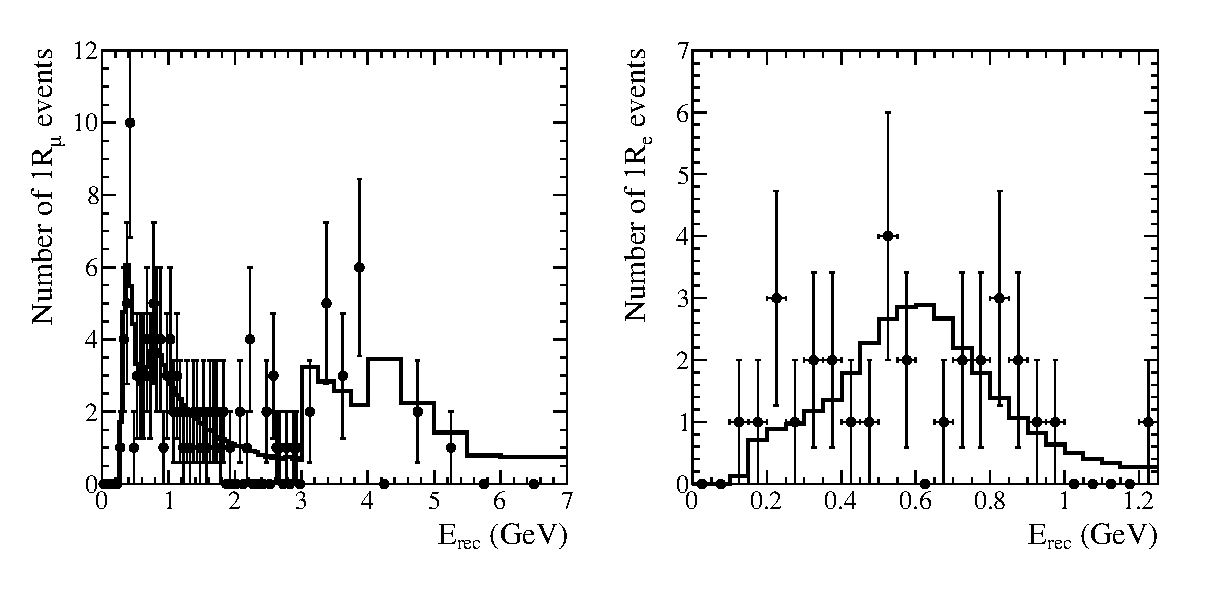
\includegraphics[width=30pc]{./images/validation/toy_dataset0_theta_fit_joint_nh_hesse_bf.eps}
\caption {
  Single $\mu$-like ring event (left) and single e-like ring event (right) best-fit reconstructed energy spectra
  to fake dataset \#0.
}
\label{fig:validation:toys:bfspectra0}
\end{center}
\vfill
\vspace*{0.7cm}
\begin{center}
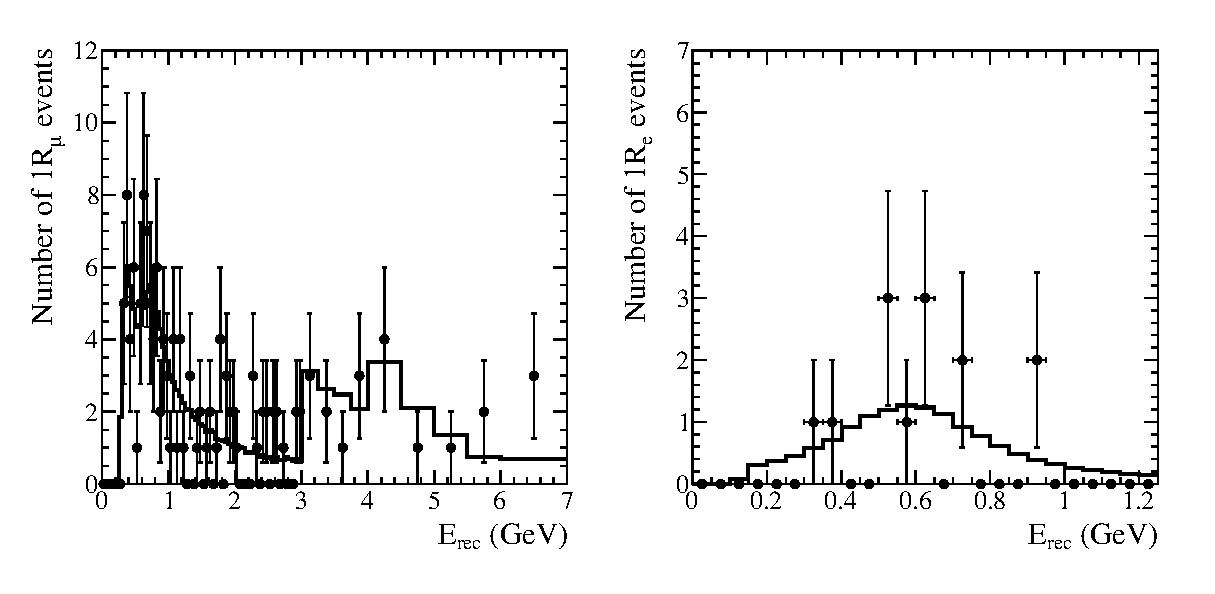
\includegraphics[width=30pc]{./images/validation/toy_dataset1_theta_fit_joint_nh_hesse_bf.eps}
\caption {
  Single $\mu$-like ring event (left) and single e-like ring event (right) best-fit reconstructed energy spectra
  to fake dataset \#1.
}
\label{fig:validation:toys:bfspectra1}
\end{center}
\vfill
\vspace*{0.7cm}
\begin{center}
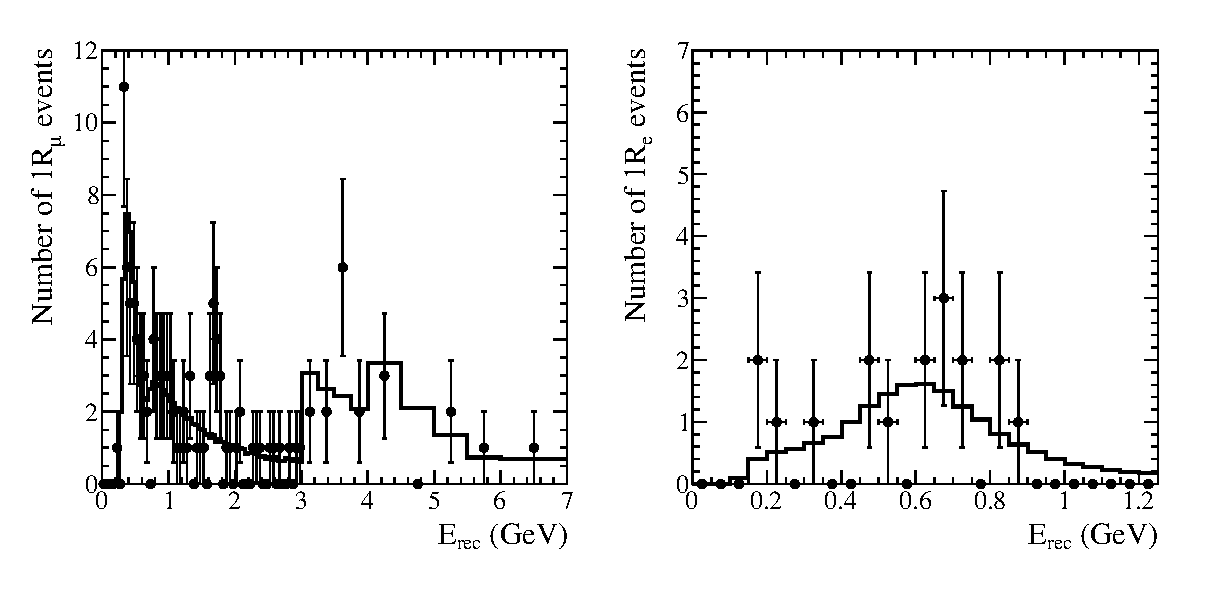
\includegraphics[width=30pc]{./images/validation/toy_dataset2_theta_fit_joint_nh_hesse_bf.eps}
\caption {
  Single $\mu$-like ring event (left) and single e-like ring event (right) best-fit reconstructed energy spectra
  to fake dataset \#2.
}
\label{fig:validation:toys:bfspectra2}
\end{center}
\end{figure*}


\begin{figure*}[htb]
\begin{center}
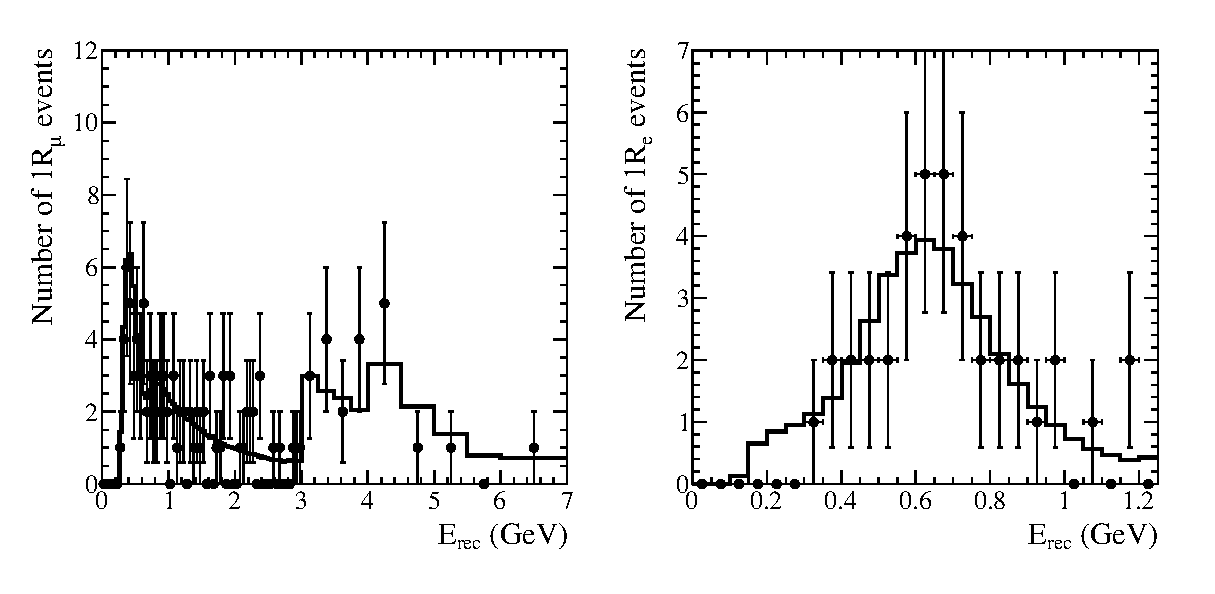
\includegraphics[width=30pc]{./images/validation/toy_dataset3_theta_fit_joint_nh_hesse_bf.eps}
\caption {
  Single $\mu$-like ring event (left) and single e-like ring event (right) best-fit reconstructed energy spectra
  to fake dataset \#3.
}
\label{fig:validation:toys:bfspectra3}
\end{center}


\vfill
\vspace*{0.7cm}
\begin{center}
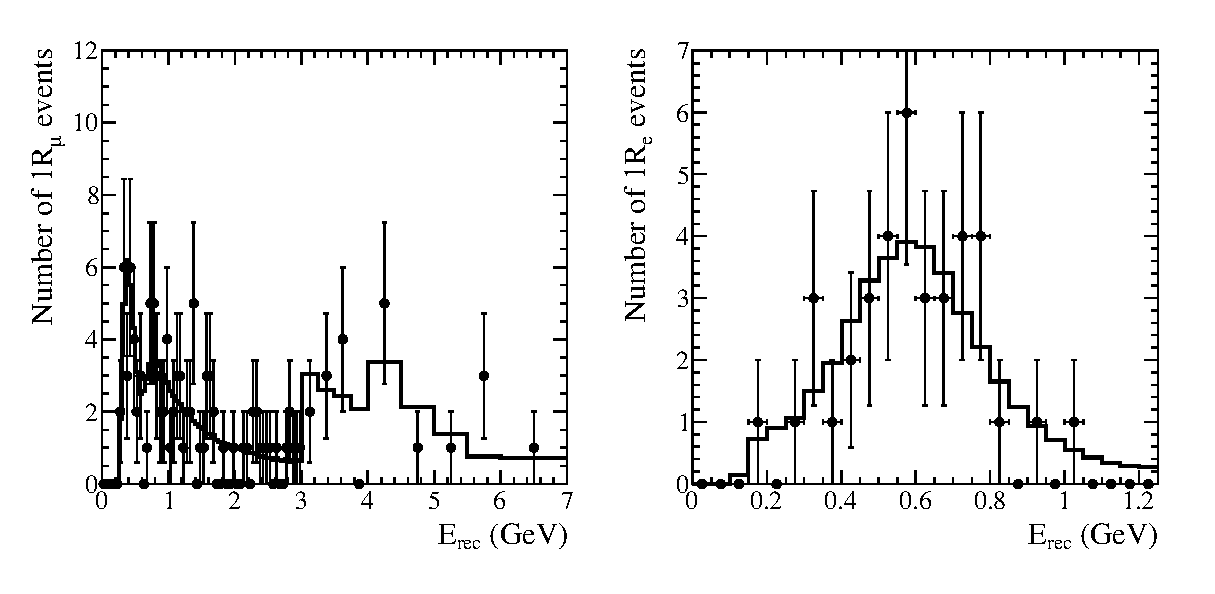
\includegraphics[width=30pc]{./images/validation/toy_dataset4_theta_fit_joint_nh_hesse_bf.eps}
\caption {
  Single $\mu$-like ring event (left) and single e-like ring event (right) best-fit reconstructed energy spectra
  to fake dataset \#4.
}
\label{fig:validation:toys:bfspectra4}
\end{center}

\vfill
\vspace*{0.7cm}
\begin{center}
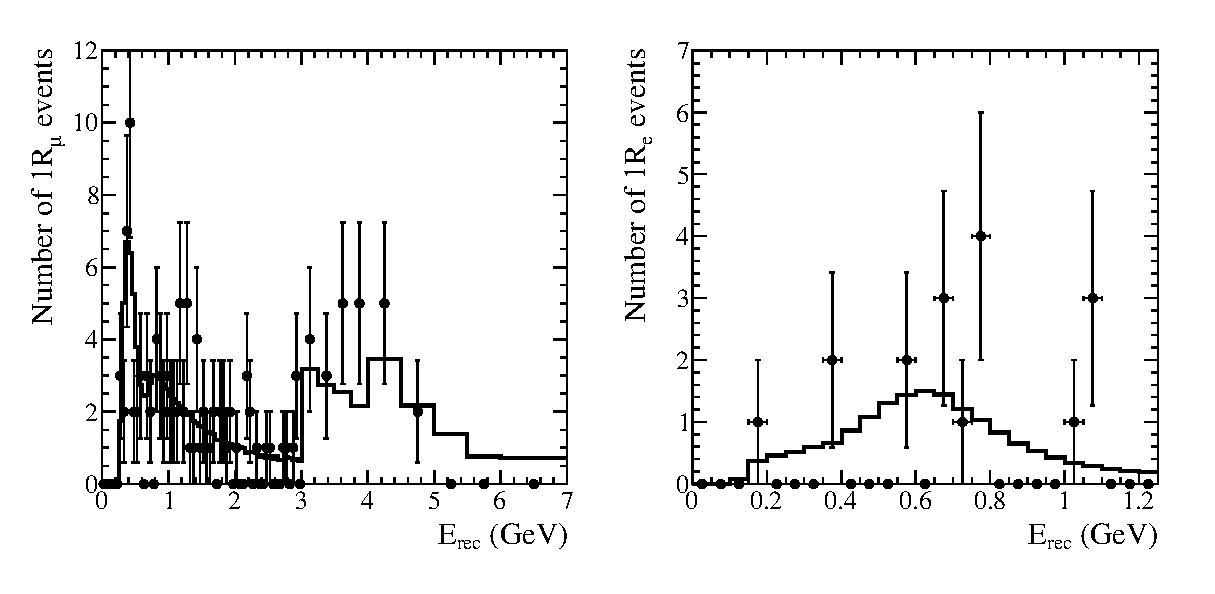
\includegraphics[width=30pc]{./images/validation/toy_dataset5_theta_fit_joint_ih_hesse_bf.eps}
\caption {
  Single $\mu$-like ring event (left) and single e-like ring event (right) best-fit reconstructed energy spectra
  to fake dataset \#5 assuming inverted hierarchy (true one).
}
\label{fig:validation:toys:bfspectra5}
\end{center}
\end{figure*}

\begin{figure*}[htb]
\begin{center}
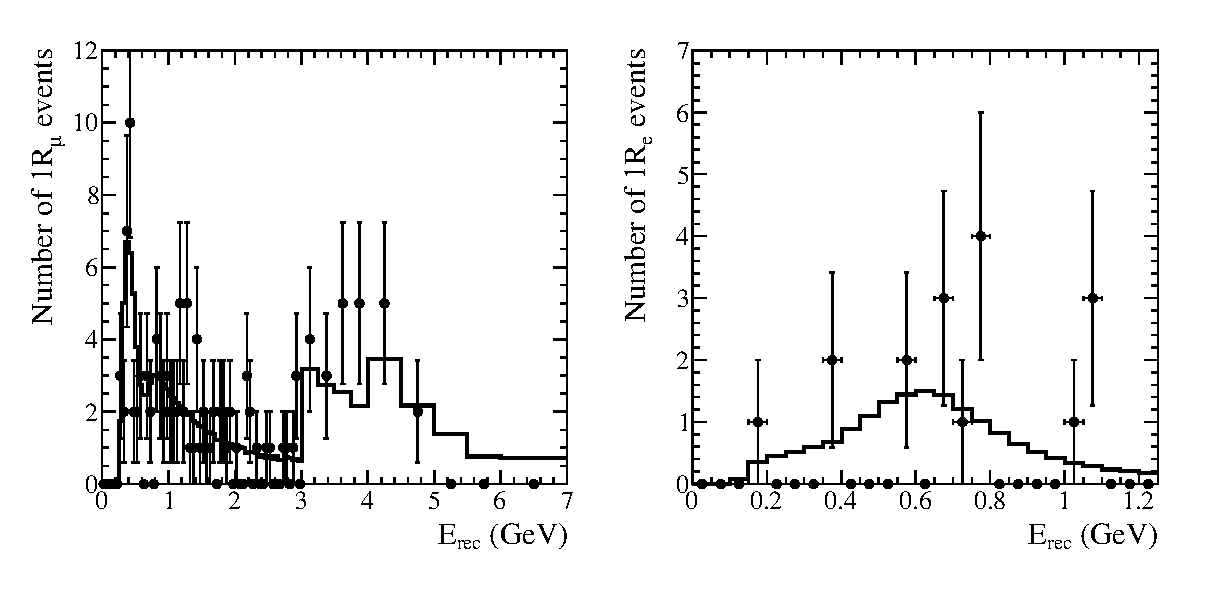
\includegraphics[width=30pc]{./images/validation/toy_dataset5_theta_fit_joint_nh_hesse_bf.eps}
\caption {
  Single $\mu$-like ring event (left) and single e-like ring event (right) best-fit reconstructed energy spectra
  to fake dataset \#5 assuming normal hierarchy. 
}
\label{fig:validation:toys:bfspectra6}
\end{center}
\vfill
\vspace*{0.7cm}
\begin{center}
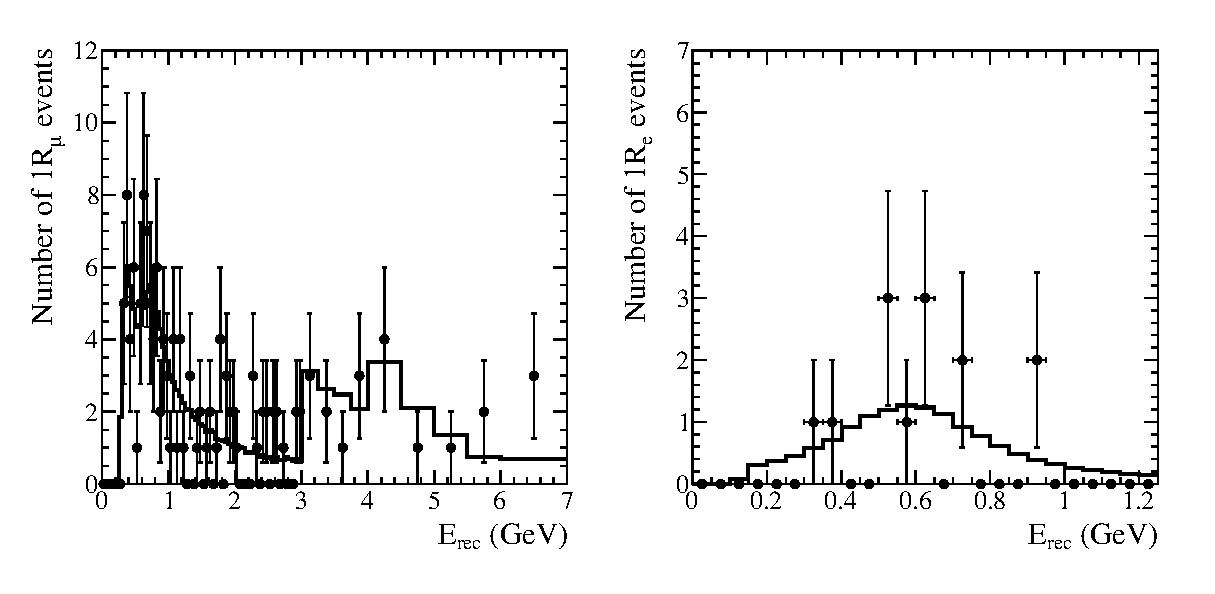
\includegraphics[width=30pc]{./images/validation/toy_dataset1_theta2theta_fit_joint_nh_hesse_bf.eps}
\caption {
  Single $\mu$-like ring event (left) and single e-like ring event (right) best-fit reconstructed energy spectra
  to fake dataset \#1 using $sin^{2}2\theta_{13}$ instead of $sin^{2}\theta_{13}$.
}
\label{fig:validation:toys:bfspectra7}
\end{center}
\end{figure*}



%%% PULLS


\begin{figure*}[htb]
\begin{center}
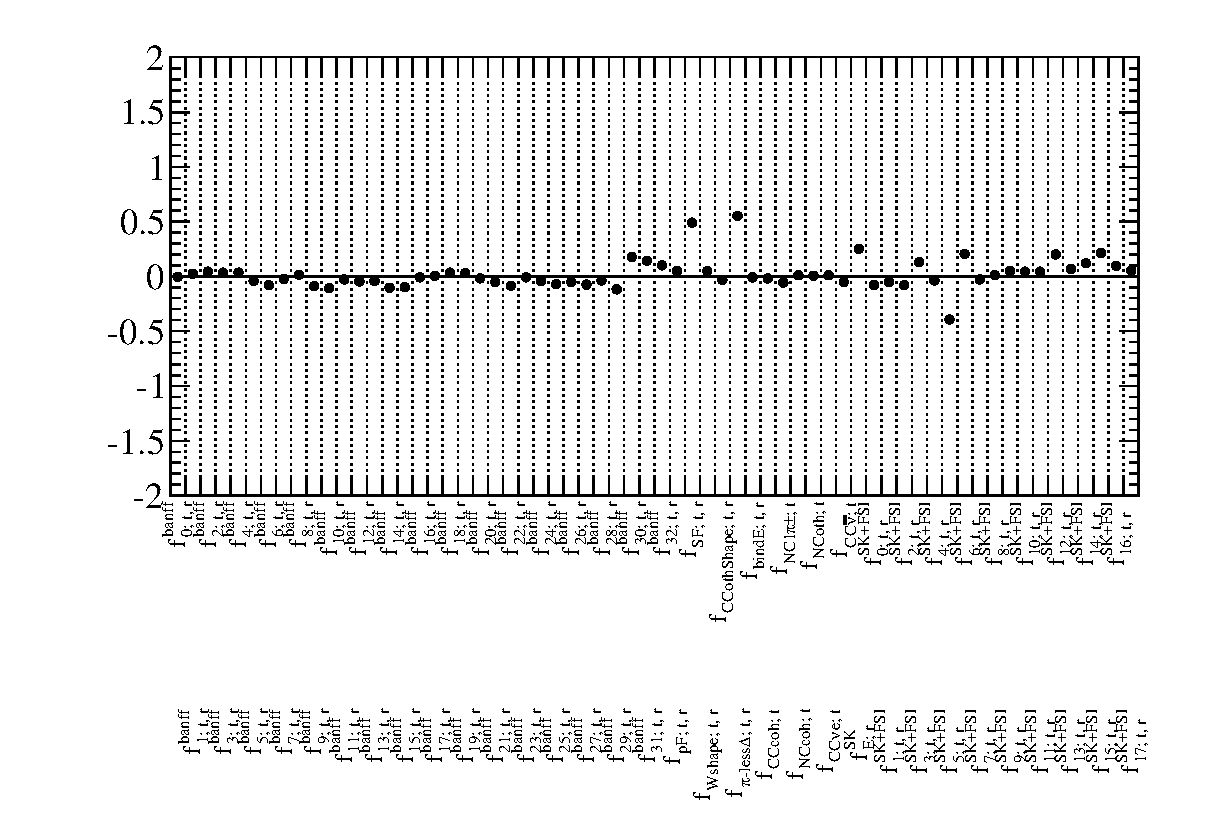
\includegraphics[width=25pc]{./images/validation/toy_dataset0_theta_fit_joint_nh_hesse_pulls.eps}
\caption {
 Systematic parameter pulls for the oscillation fit to fake dataset \#0.
}
\label{fig:validation:toys:pulls0}
\end{center}
\vfill
\vspace*{0.7cm}
\begin{center}
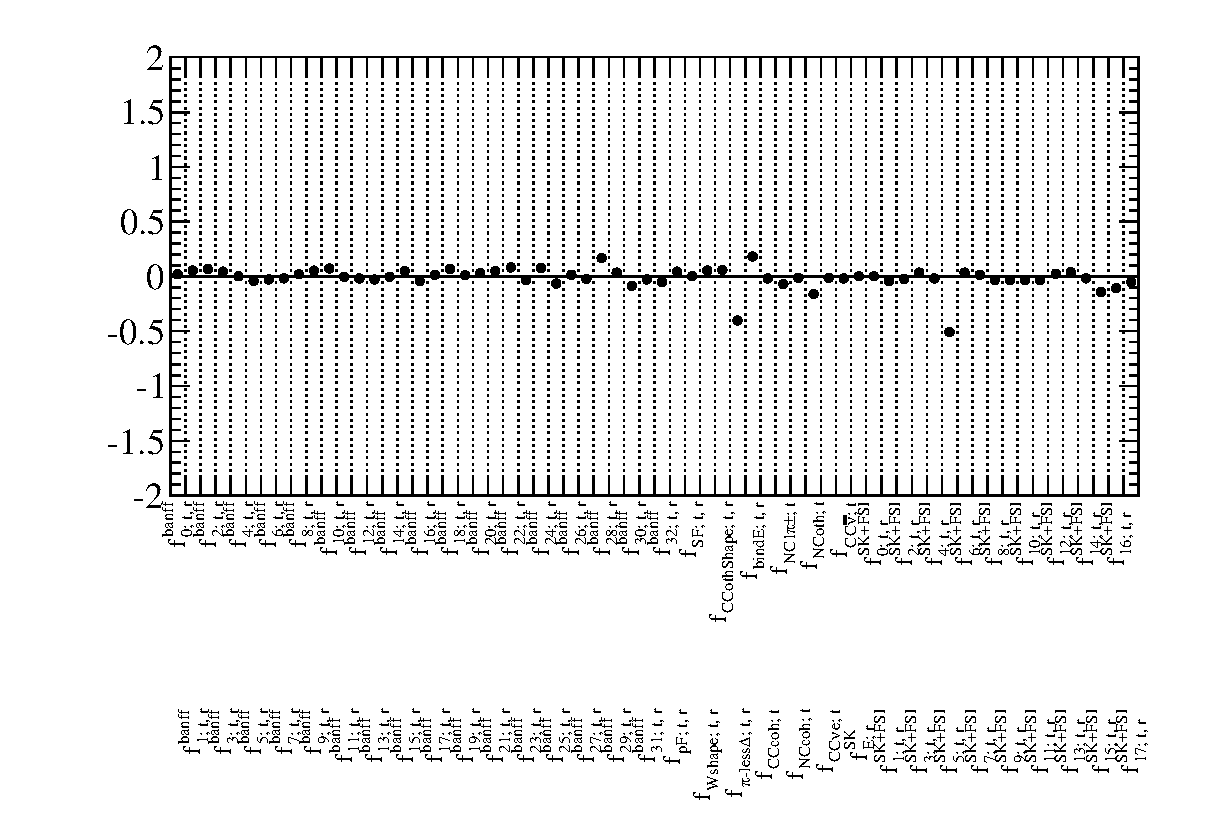
\includegraphics[width=25pc]{./images/validation/toy_dataset1_theta_fit_joint_nh_hesse_pulls.eps}
\caption {
 Systematic parameter pulls for the oscillation fit to fake dataset \#1.
}
\label{fig:validation:toys:pulls1}
\end{center}
\vfill
\vspace*{0.7cm}

\begin{center}
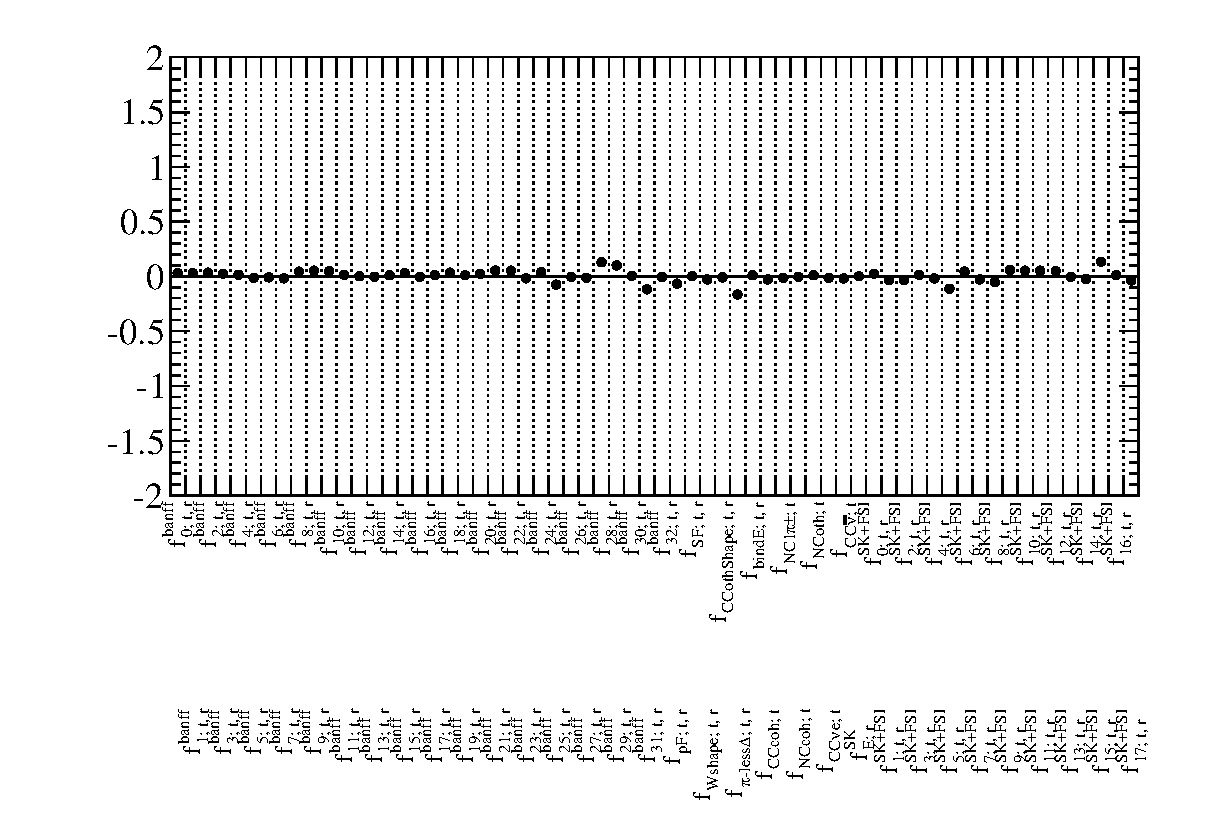
\includegraphics[width=25pc]{./images/validation/toy_dataset2_theta_fit_joint_nh_hesse_pulls.eps}
\caption {
 Systematic parameter pulls for the oscillation fit to fake dataset \#2.
}
\label{fig:validation:toys:pulls2}
\end{center}

\end{figure*}

\begin{figure*}[htb]
\begin{center}
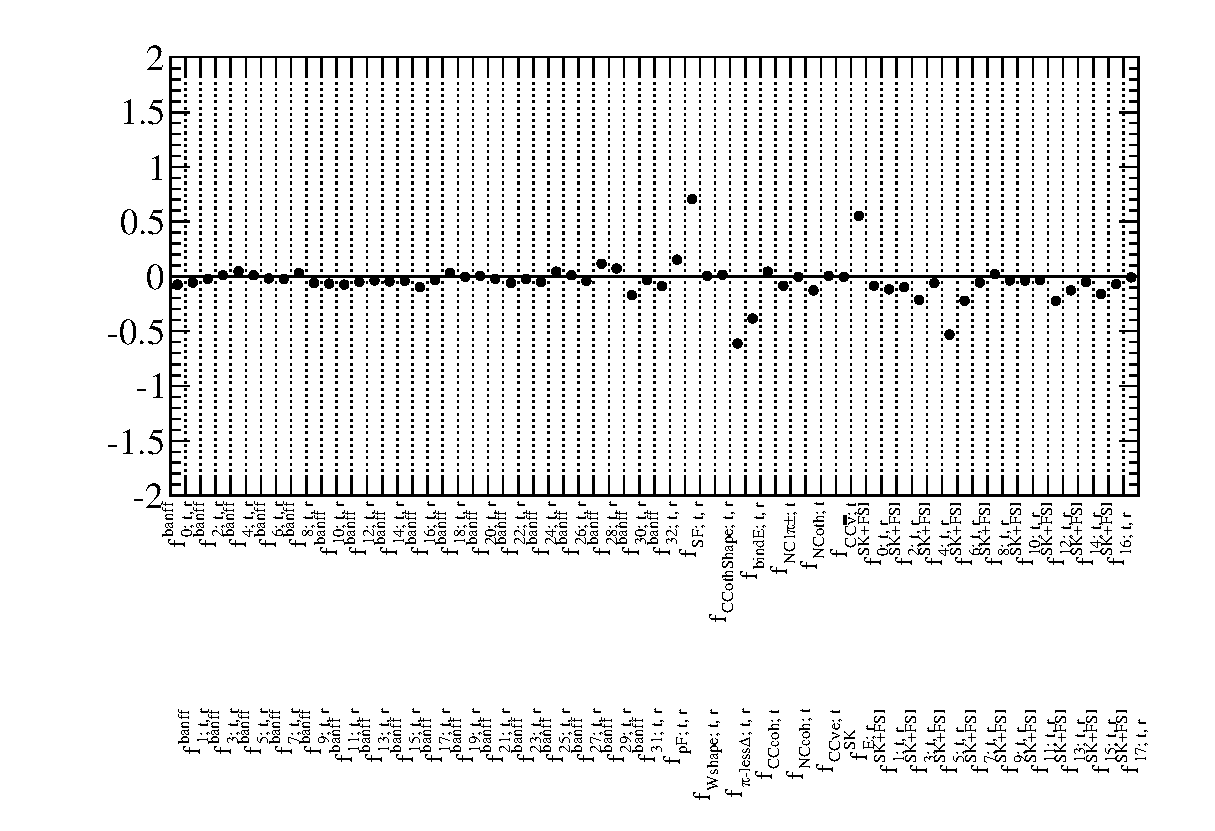
\includegraphics[width=25pc]{./images/validation/toy_dataset3_theta_fit_joint_nh_hesse_pulls.eps}
\caption {
 Systematic parameter pulls for the oscillation fit to fake dataset \#3.
}
\label{fig:validation:toys:pulls3}
\end{center}
\vfill
\vspace*{0.7cm}
\begin{center}
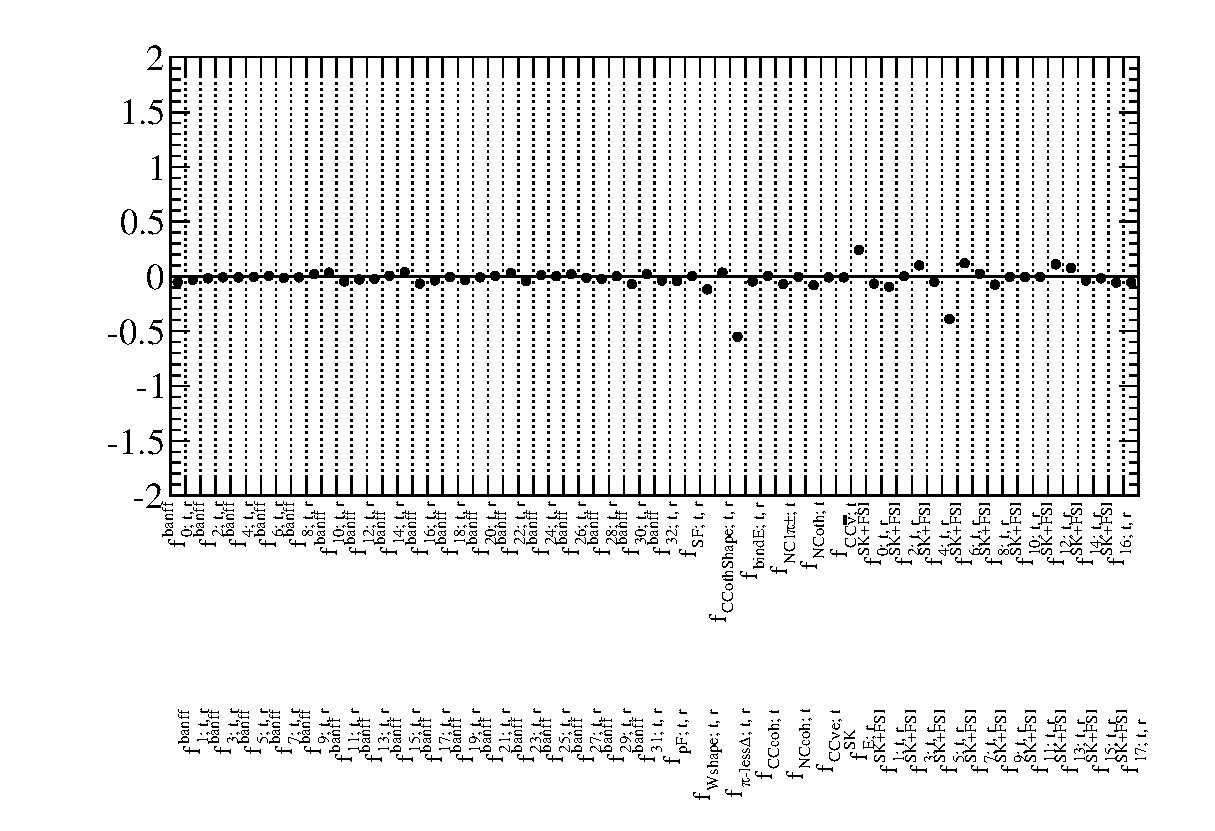
\includegraphics[width=25pc]{./images/validation/toy_dataset4_theta_fit_joint_nh_hesse_pulls.eps}
\caption {
 Systematic parameter pulls for the oscillation fit to fake dataset \#4.
}
\label{fig:validation:toys:pulls4}
\end{center}
\vfill
\vspace*{0.7cm}

\begin{center}
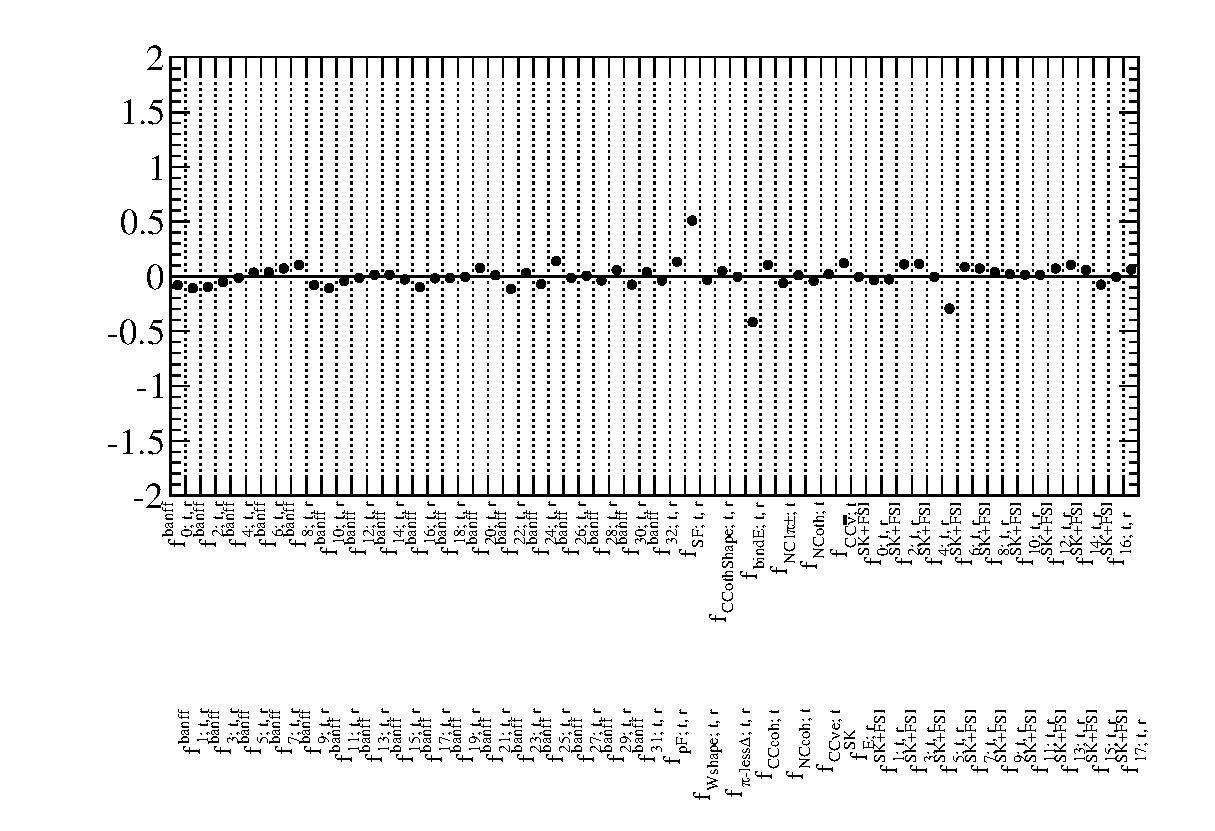
\includegraphics[width=25pc]{./images/validation/toy_dataset5_theta_fit_joint_ih_hesse_pulls.eps}
\caption {
 Systematic parameter pulls for the oscillation fit to fake dataset \#5 assuming inverted hierarchy (true one).
}
\label{fig:validation:toys:pulls5}
\end{center}

\end{figure*}

\begin{figure*}[htb]
\begin{center}
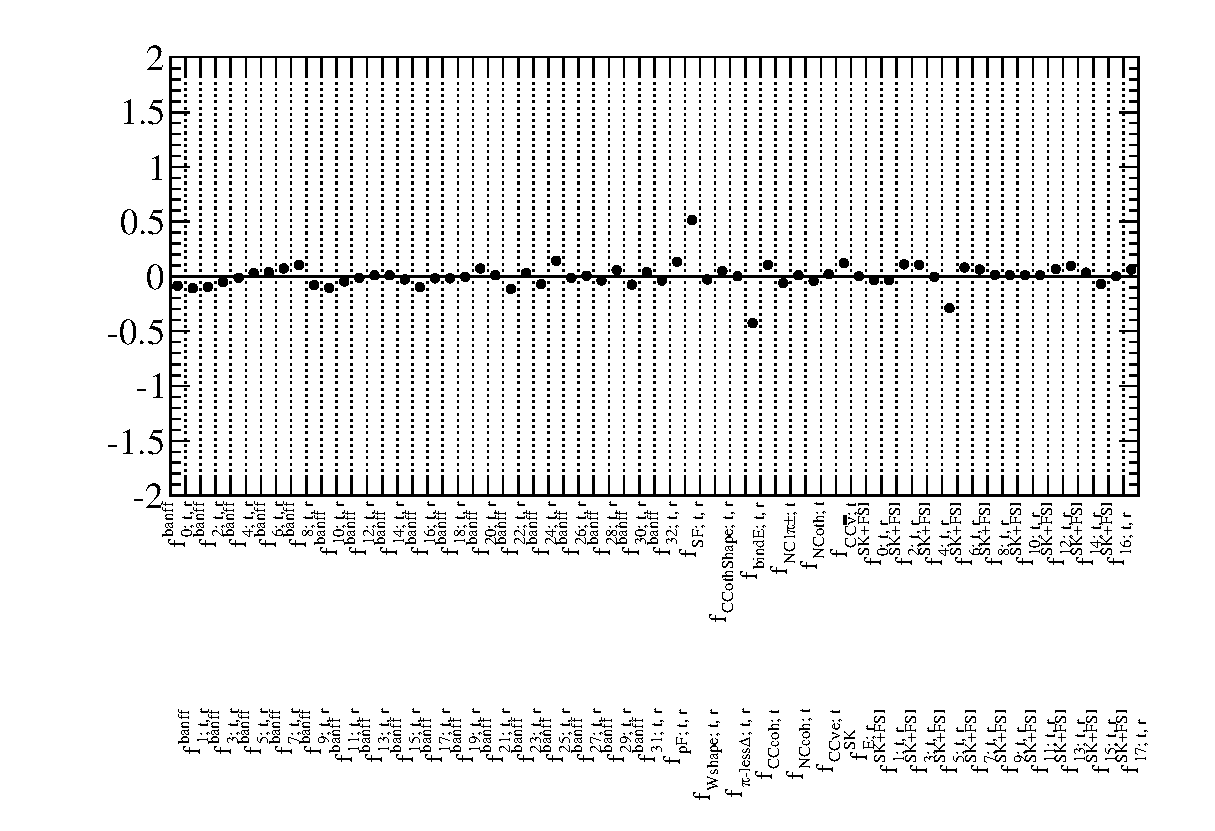
\includegraphics[width=25pc]{./images/validation/toy_dataset5_theta_fit_joint_nh_hesse_pulls.eps}
\caption {
 Systematic parameter pulls for the oscillation fit to fake dataset \#5 assuming normal hierarchy.
}
\label{fig:validation:toys:pulls6}
\end{center}
\vfill
\vspace*{0.7cm}

\begin{center}
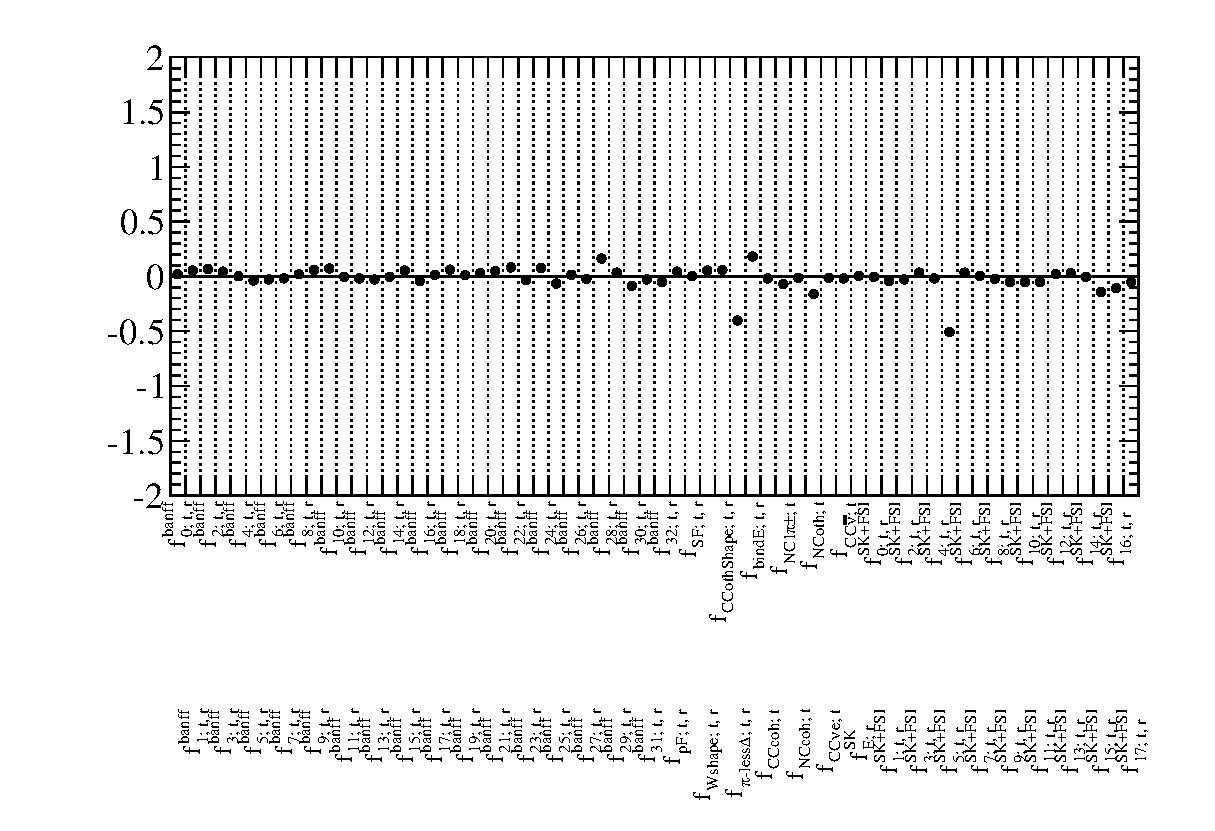
\includegraphics[width=25pc]{./images/validation/toy_dataset1_theta2theta_fit_joint_nh_hesse_pulls.eps}
\caption {
 Systematic parameter pulls for the oscillation fit to fake dataset \#1 using $sin^{2}2\theta_{13}$ instead of $sin^{2}\theta_{13}$.
}
\label{fig:validation:toys:pulls7}
\end{center}
\end{figure*}


% 
% 
% ..............................................
% Fake dataset #0
% 
%
\clearpage

\begin{figure*}[htb]

\begin{center}
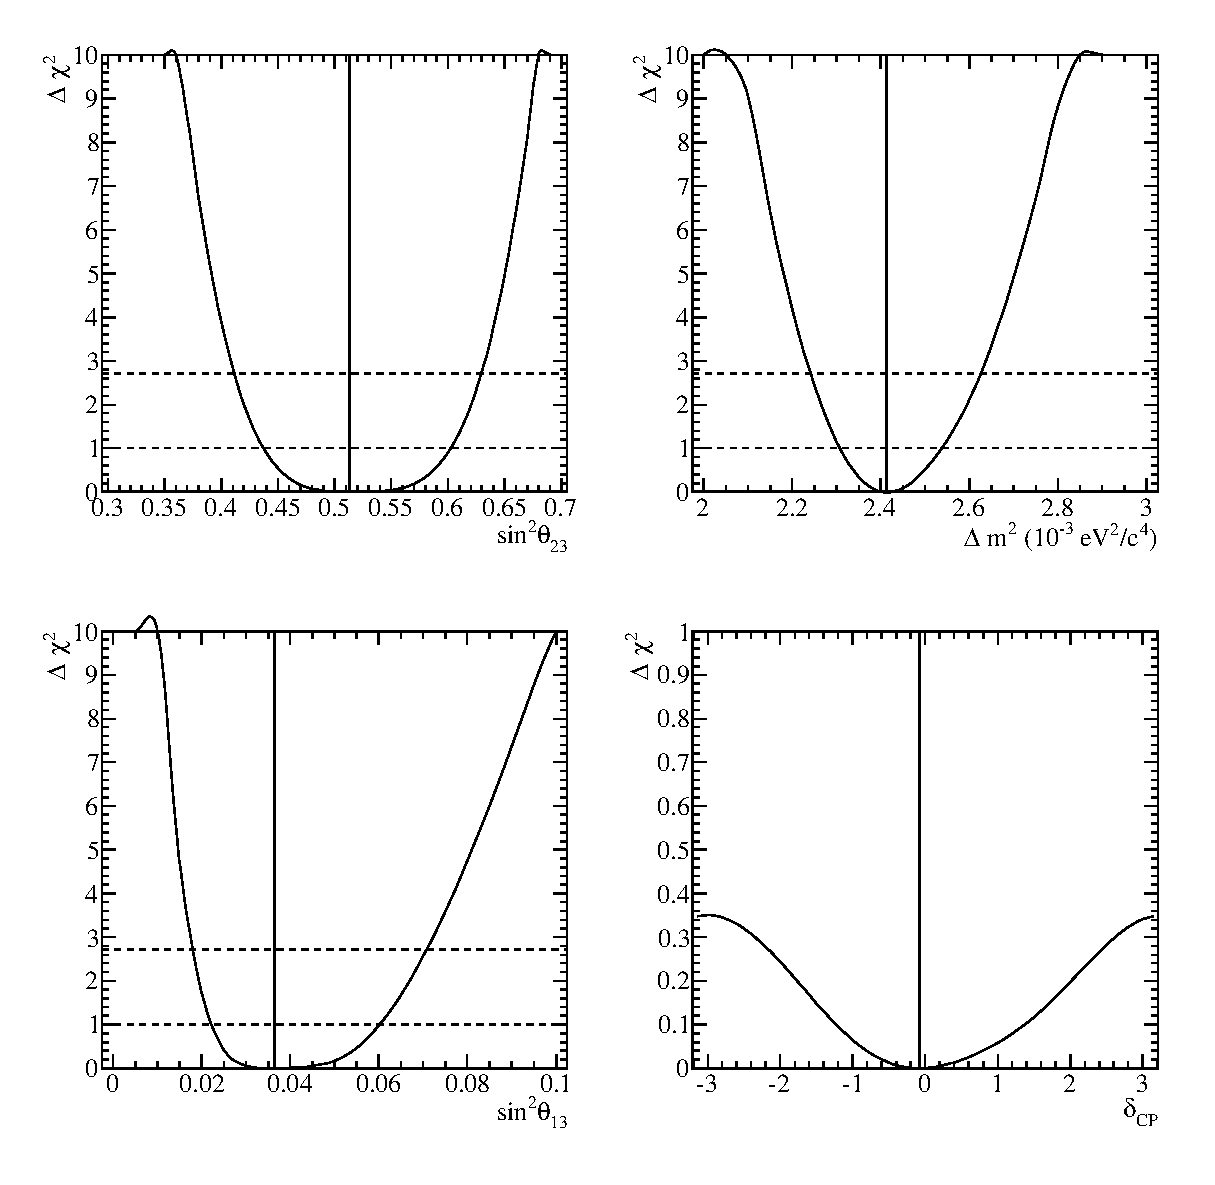
\includegraphics[width=25pc]{./images/validation/toy_dataset0_1D.eps}
\caption {
 $\Delta\chi^2$ as function of $\sin^{2}\theta_{23}$,$|\Delta m^{2}|$,$\sin^{2}\theta_{13}$ and $\delta_{CP}$
for fake dataset \#0.
  At each point, $\chi^2$ was minimized with respect to the oscillation parameters not shown in each figure
and all 64 systematic parameters.
}
\label{fig:validation:toys:1D_toy0}
\end{center}
\vfill
\vspace*{0.7cm}

\begin{center}
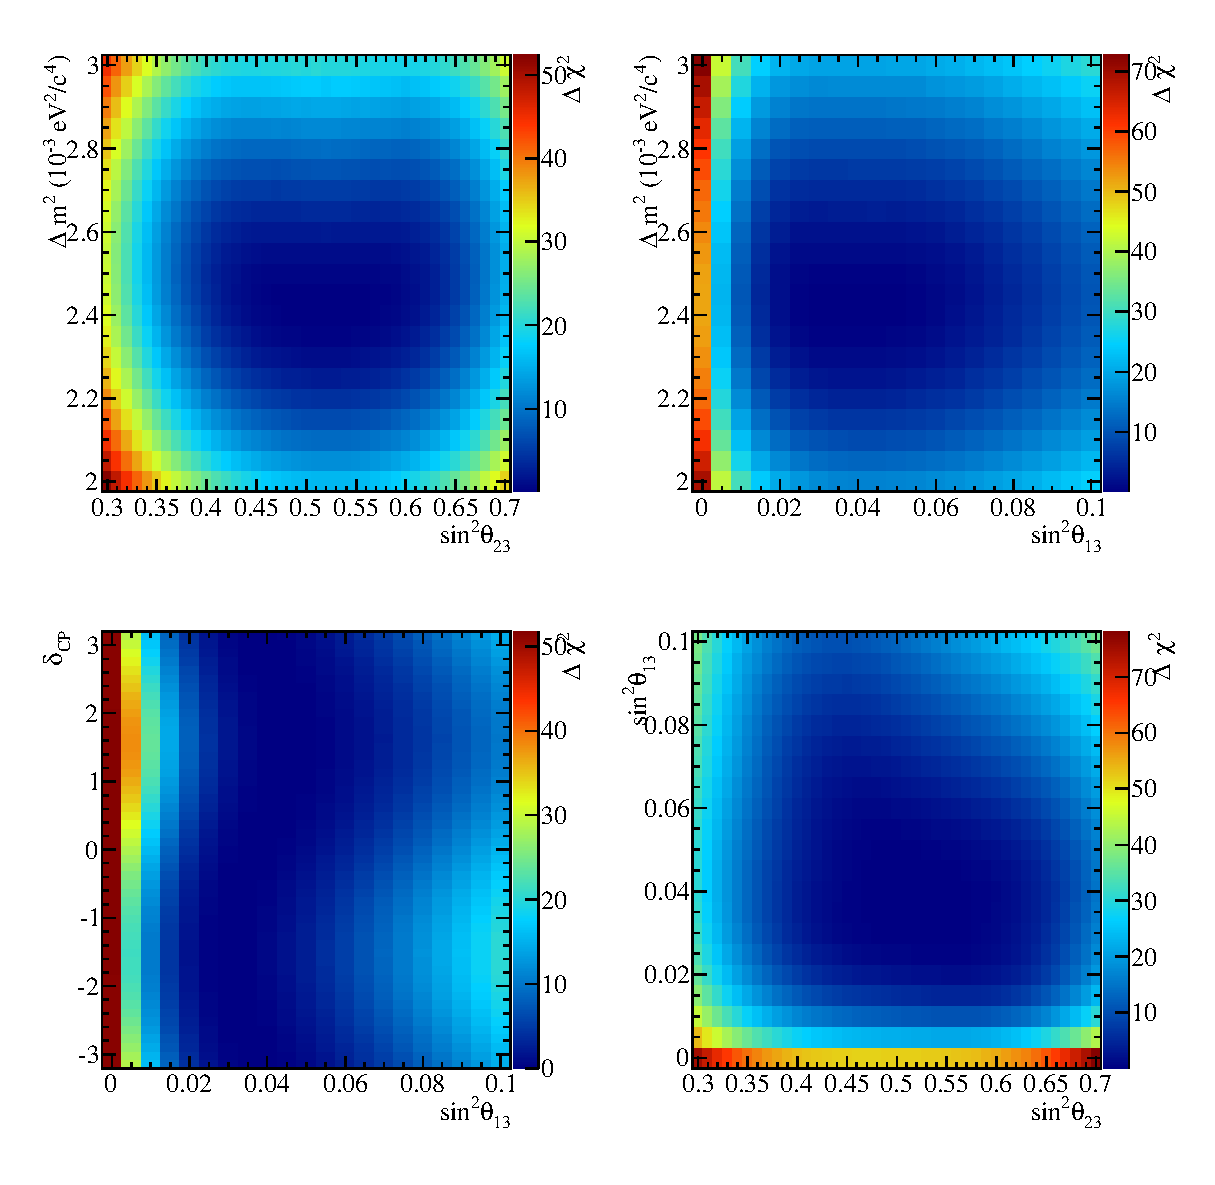
\includegraphics[width=30pc]{./images/validation/toy_dataset0_colz.eps}
\caption {
  $\Delta\chi^2$ surface in
($|\Delta m^{2}|$,$sin^{2}\theta_{23}$), 
($|\Delta m^{2}|$,$sin^{2}\theta_{13}$), 
($\delta_{CP}$,$sin^{2}\theta_{13}$) and 
($sin^{2}\theta_{13}$,$sin^{2}\theta_{23}$)
 spaces for fake dataset \#0.
At each point, $\chi^2$ was minimized with respect to the oscillation parameters not shown in each figure
and all 64 systematic parameters.
}
\label{fig:validation:toys:colz_toy0}

\end{center}
\end{figure*}


\begin{figure*}[htb]



\begin{center}
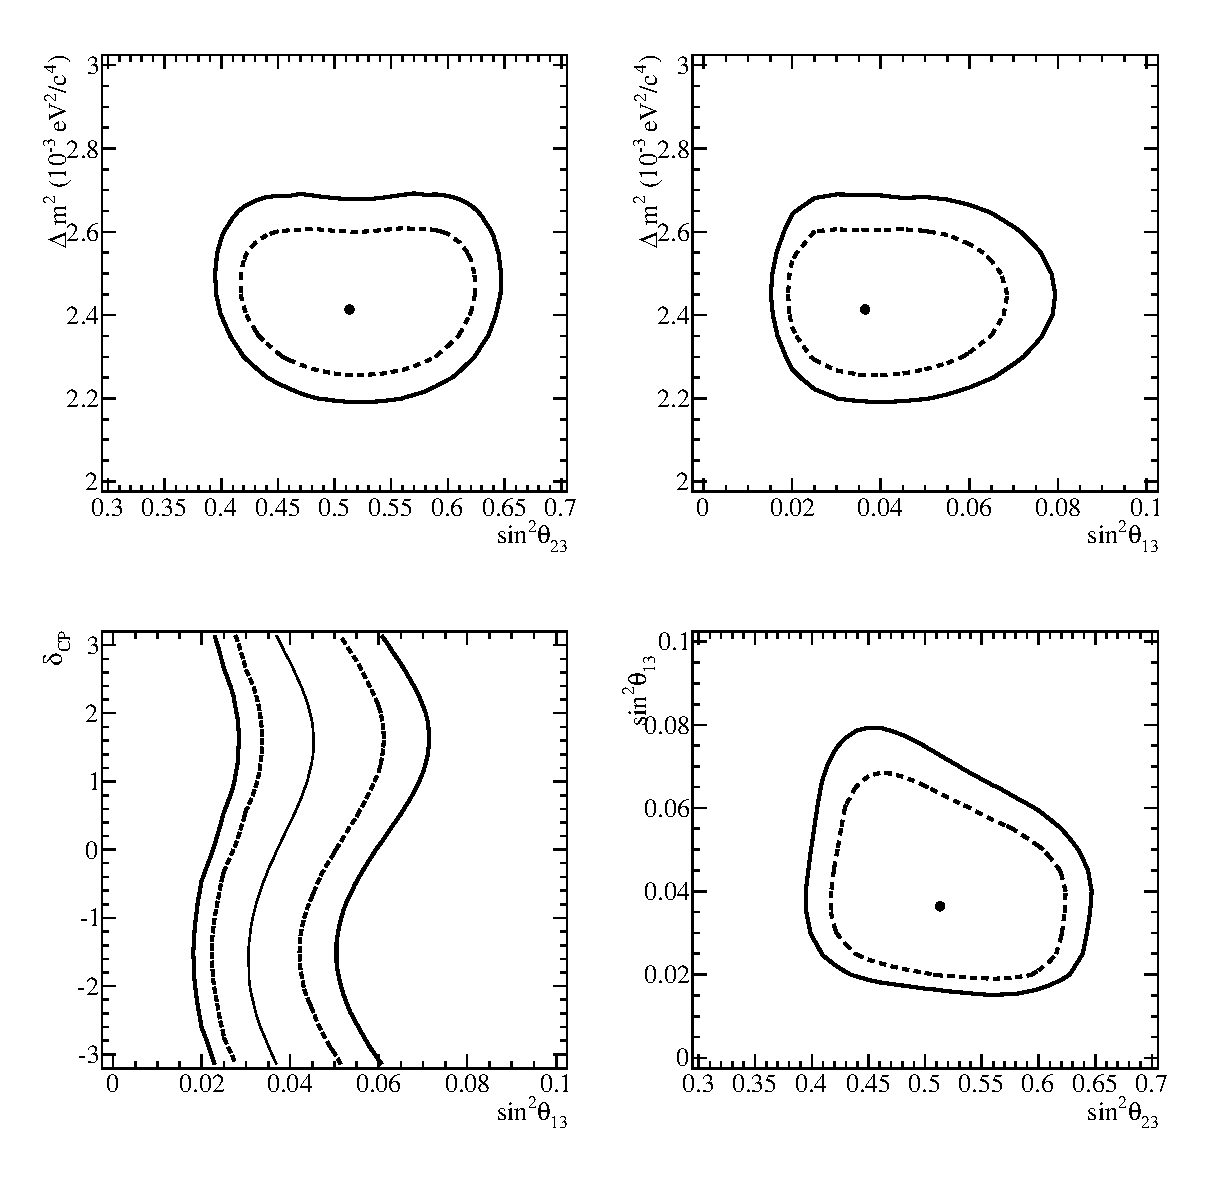
\includegraphics[width=40pc]{./images/validation/toy_dataset0_2D.eps}
\caption {
 68\% and 90\% CL regions in 
($|\Delta m^{2}|$,$sin^{2}\theta_{23}$), 
($|\Delta m^{2}|$,$sin^{2}\theta_{13}$), 
($\delta_{CP}$,$sin^{2}\theta_{13}$) and 
($sin^{2}\theta_{13}$,$sin^{2}\theta_{23}$)
 spaces for fake dataset \#0.
At each point, $\chi^2$ was minimized with respect to the oscillation parameters not shown in each figure
and all 64 systematic parameters.
}
\label{fig:validation:toys:2D_toy0}
\end{center}
\end{figure*}


\begin{figure*}[htb]
\begin{center}
\begin{minipage}[t]{0.48\linewidth}

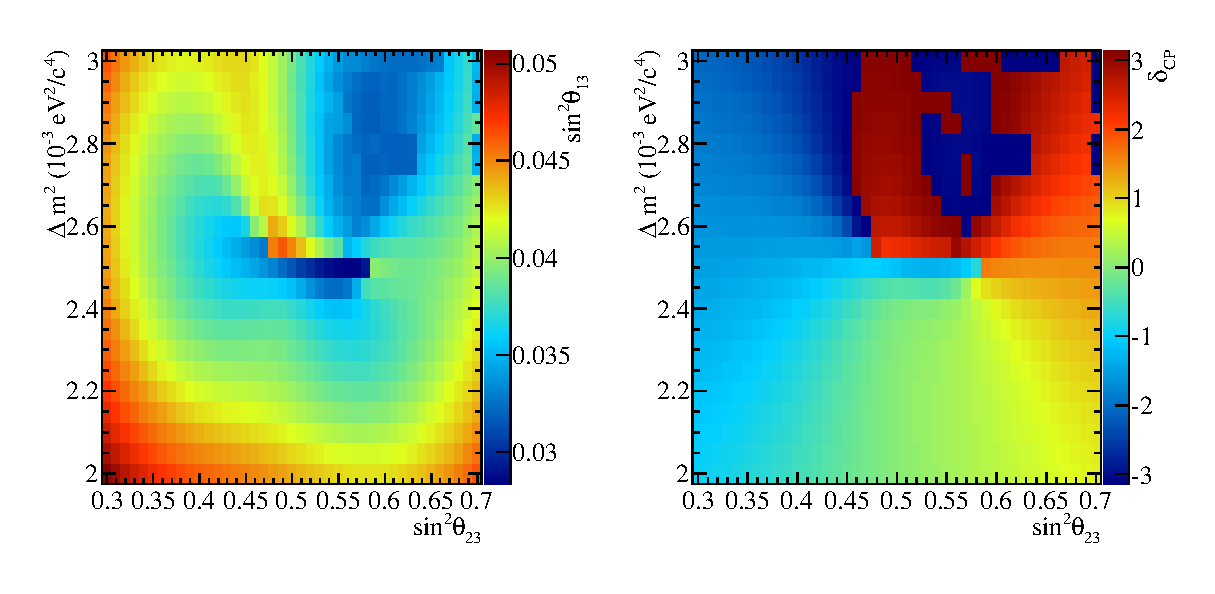
\includegraphics[width=10cm]{./images/validation/toy_dataset0_theta23_dmsq_extra.eps}
\caption {
 Best fit value of $sin^{2}\theta_{13}$ and $\delta_{CP}$
for the fit in the ($|\Delta m^{2}|$,$sin^{2}\theta_{23}$) space
for fake dataset \#0.
}

\end{minipage}
\end{center}
\vfill
\vspace*{0.5cm}
\begin{center}
\begin{minipage}[t]{0.48\linewidth}

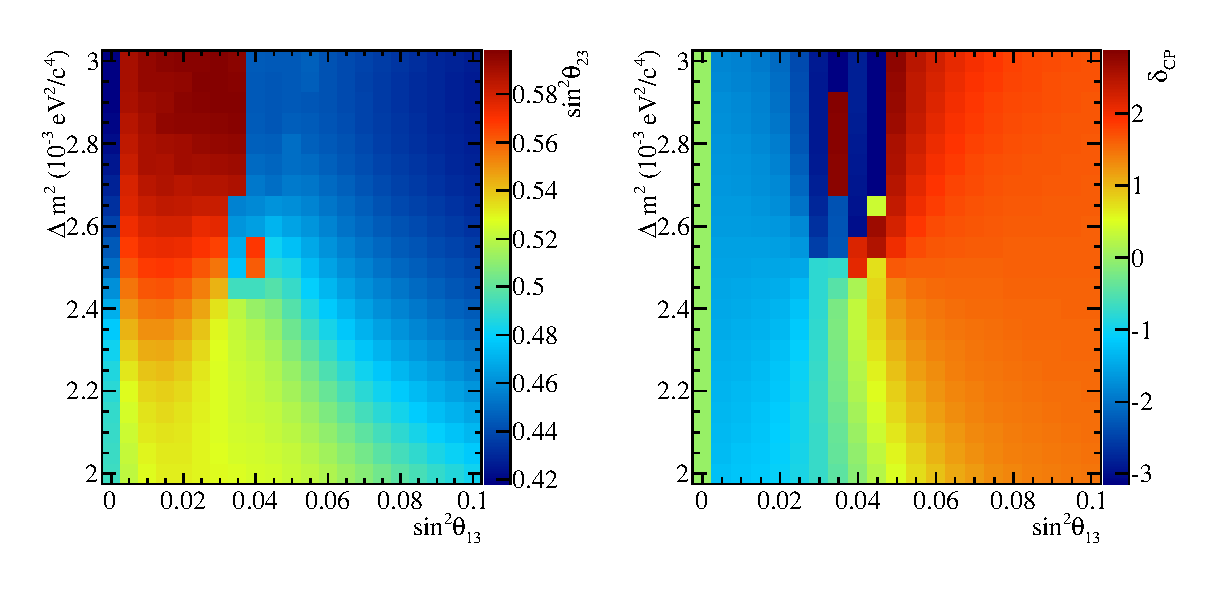
\includegraphics[width=10cm]{./images/validation/toy_dataset0_theta13_dmsq_extra.eps}
\caption {
 Best fit value of $sin^{2}\theta_{23}$ and $\delta_{CP}$
for the fit in the ($|\Delta m^{2}|$,$sin^{2}\theta_{13}$) space
for fake dataset \#0.
}

\end{minipage}
\end{center}
\vfill
\vspace*{0.5cm}
\begin{center}
\begin{minipage}[t]{0.48\linewidth}

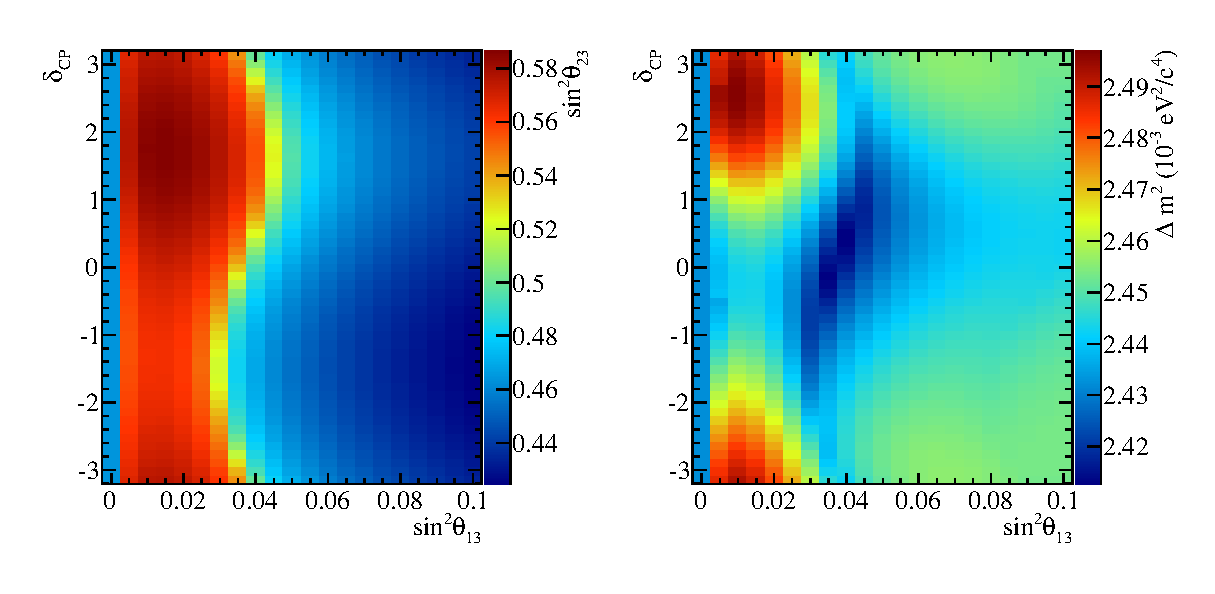
\includegraphics[width=10cm]{./images/validation/toy_dataset0_theta13_deltacp_extra.eps}
\caption {
 Best fit value of $sin^{2}\theta_{23}$ and $|\Delta m^{2}|$ 
for the fit in the ($\delta_{CP}$,$sin^{2}\theta_{23}$) space
for fake dataset \#0.
}

\end{minipage}
\end{center}

\vfill
\vspace*{0.5cm}
\begin{center}
\begin{minipage}[t]{0.48\linewidth}

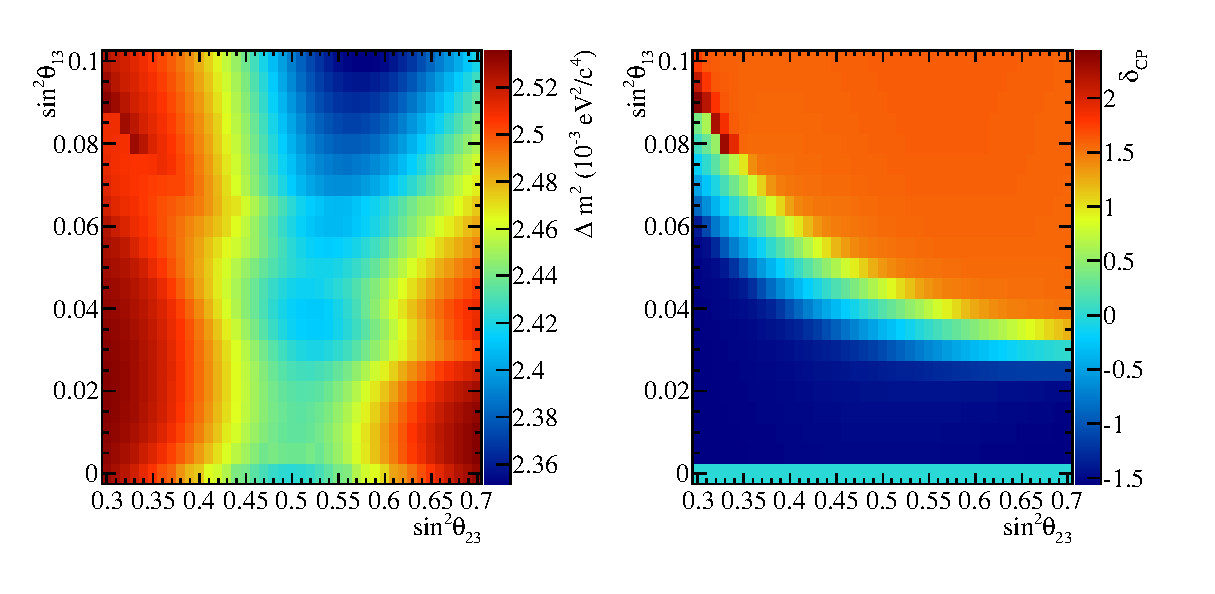
\includegraphics[width=10cm]{./images/validation/toy_dataset0_theta13_theta23_extra.eps}
\caption {
 Best fit value of $\delta_{CP}$ and $|\Delta m^{2}|$ 
for the fit in the ($sin^{2}\theta_{23}$,$sin^{2}\theta_{13}$) space
for fake dataset \#0.
}

\end{minipage}
\end{center}

\label{fig:validation:toys:extra_toy0}
\end{figure*}


% 
% 
% ..............................................
% Fake dataset #1
% 
%
\clearpage

\begin{figure*}[htb]

\begin{center}
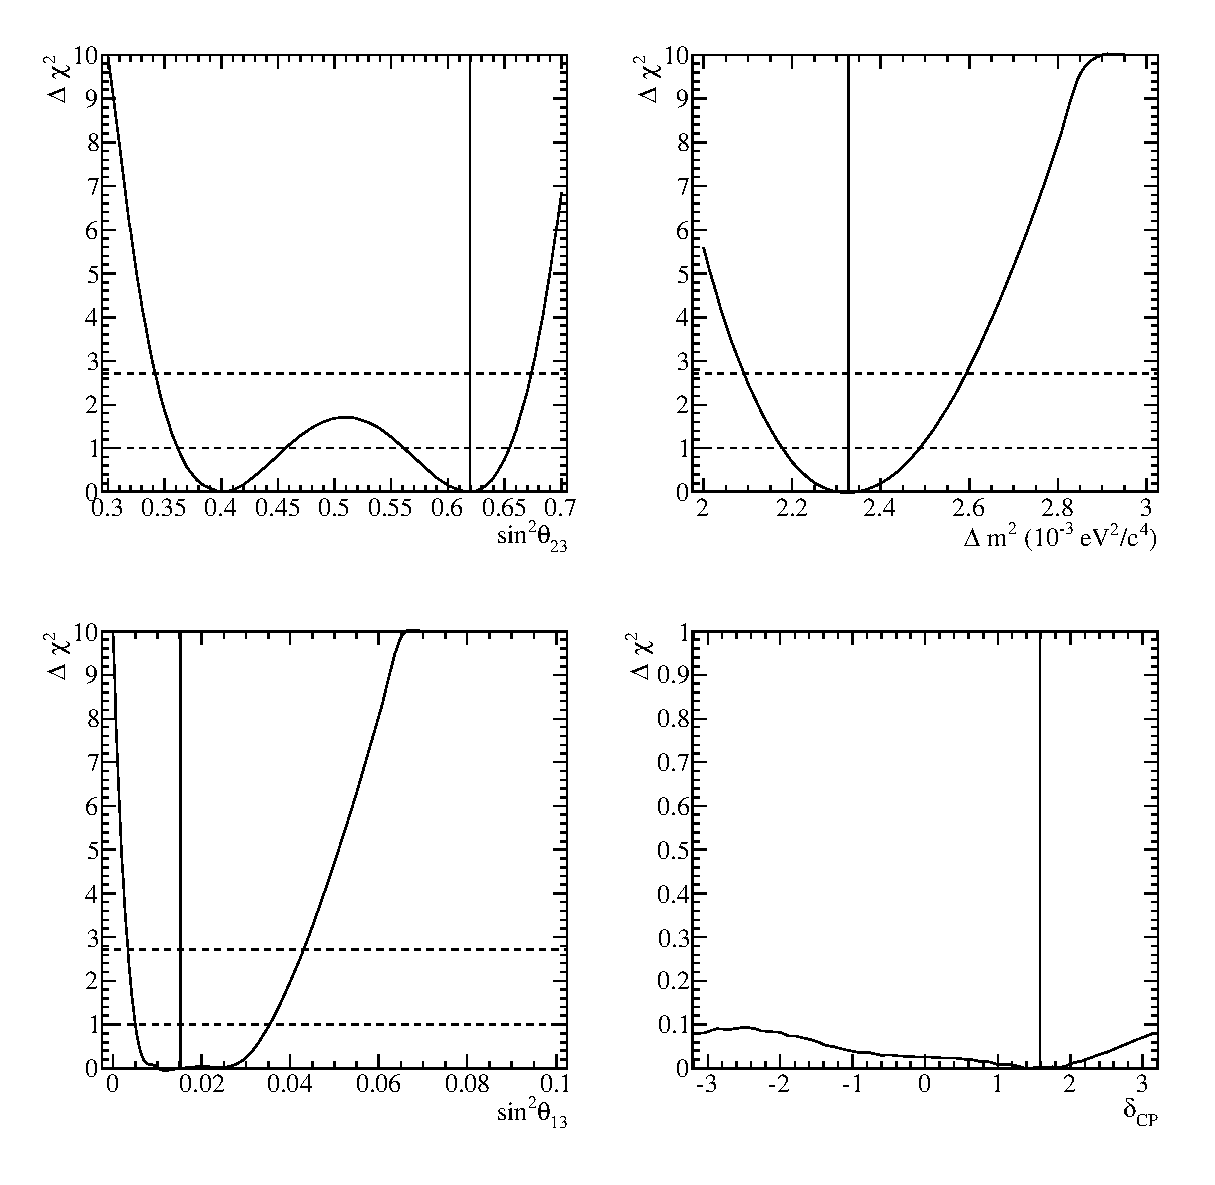
\includegraphics[width=25pc]{./images/validation/toy_dataset1_1D.eps}
\caption {
 $\Delta\chi^2$ as function of $\sin^{2}\theta_{23}$,$|\Delta m^{2}|$,$\sin^{2}\theta_{13}$ and $\delta_{CP}$
for fake dataset \#1.
  At each point, $\chi^2$ was minimized with respect to the oscillation parameters not shown in each figure
and all 64 systematic parameters.
}
\label{fig:validation:toys:1D_toy1}
\end{center}

\vfill
\vspace*{0.7cm}

\begin{center}
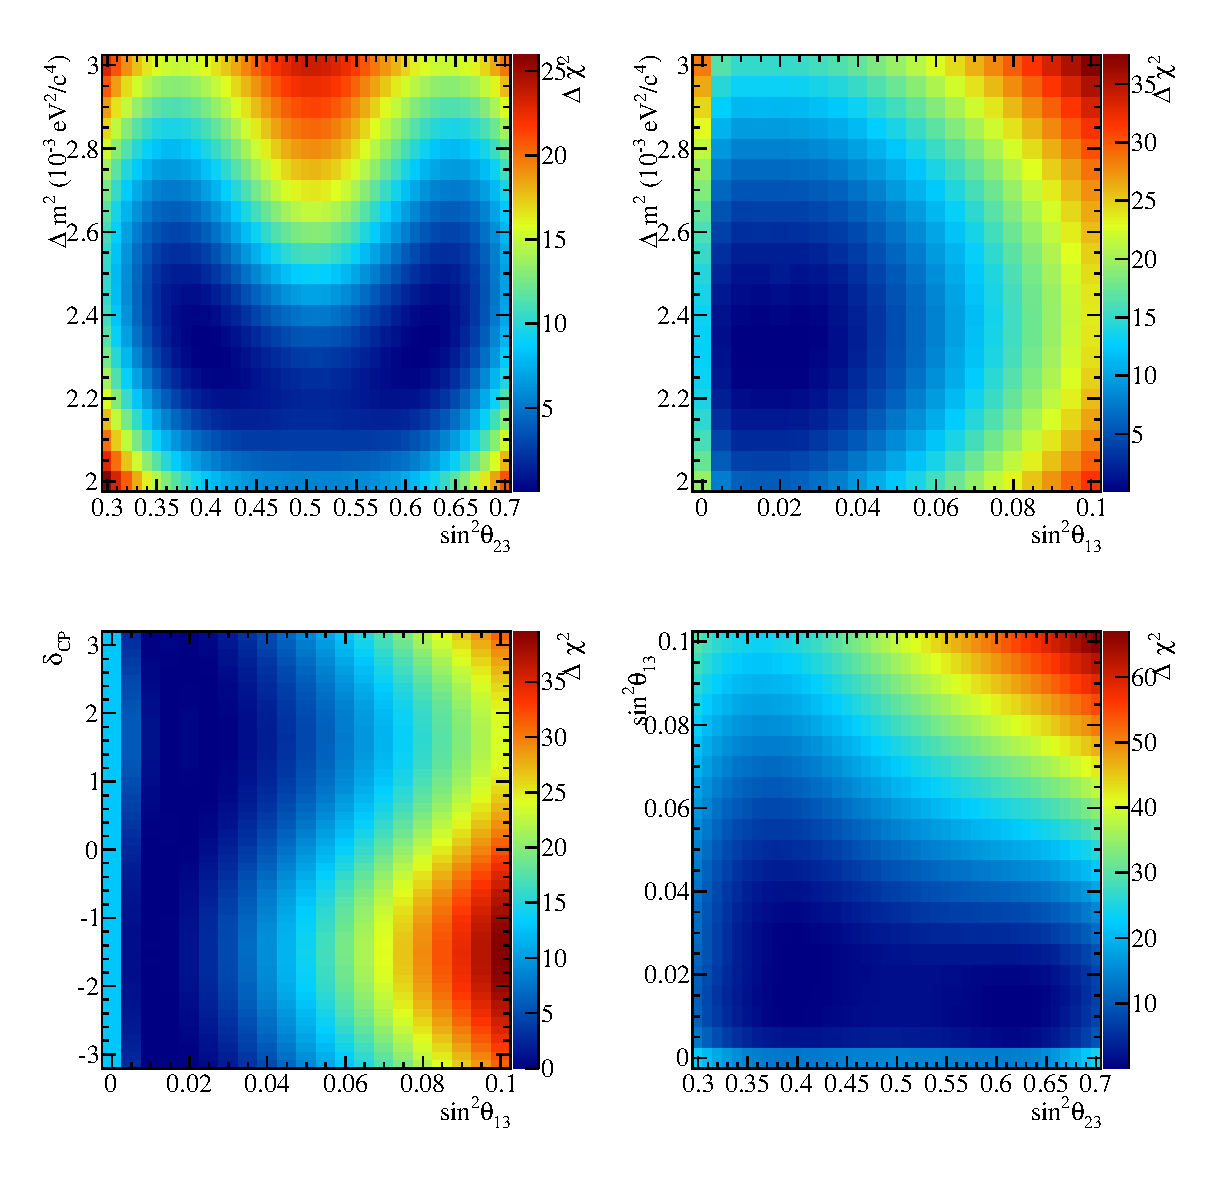
\includegraphics[width=30pc]{./images/validation/toy_dataset1_colz.eps}
\caption {
  $\Delta\chi^2$ surface in
($|\Delta m^{2}|$,$sin^{2}\theta_{23}$), 
($|\Delta m^{2}|$,$sin^{2}\theta_{13}$), 
($\delta_{CP}$,$sin^{2}\theta_{13}$) and 
($sin^{2}\theta_{13}$,$sin^{2}\theta_{23}$)
 spaces for fake dataset \#1.
At each point, $\chi^2$ was minimized with respect to the oscillation parameters not shown in each figure
and all 64 systematic parameters.
}
\label{fig:validation:toys:colz_toy1}

\end{center}

\end{figure*}


\begin{figure*}[htb]

\begin{center}
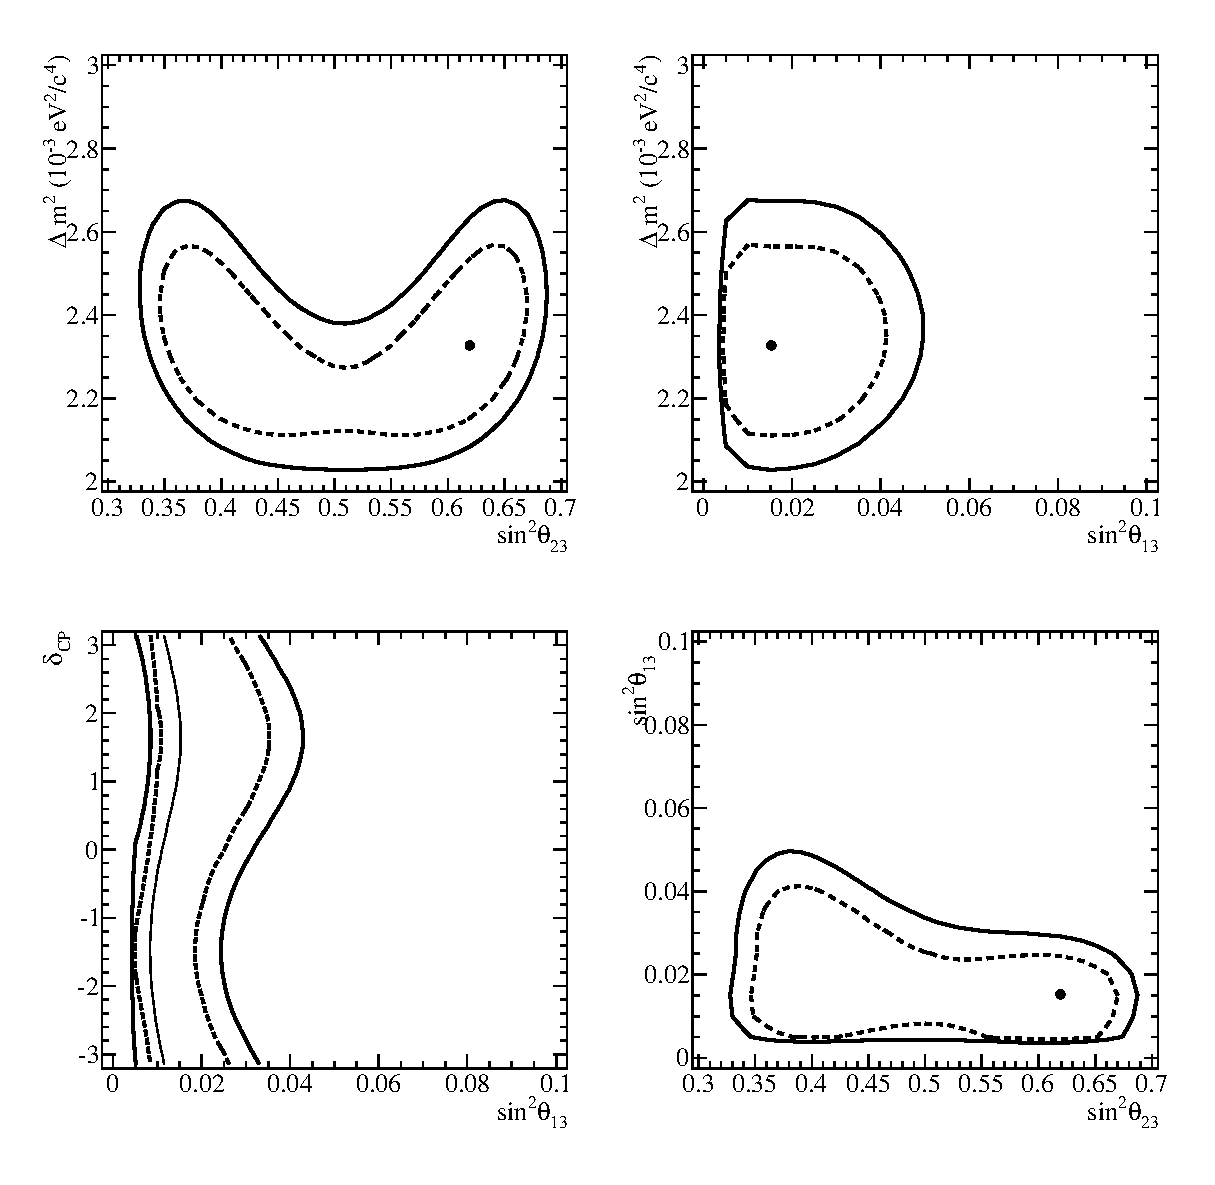
\includegraphics[width=40pc]{./images/validation/toy_dataset1_2D.eps}
\caption {
 68\% and 90\% CL regions in 
($|\Delta m^{2}|$,$sin^{2}\theta_{23}$), 
($|\Delta m^{2}|$,$sin^{2}\theta_{13}$), 
($\delta_{CP}$,$sin^{2}\theta_{13}$) and 
($sin^{2}\theta_{13}$,$sin^{2}\theta_{23}$)
 spaces for fake dataset \#1.
At each point, $\chi^2$ was minimized with respect to the oscillation parameters not shown in each figure
and all 64 systematic parameters.
}
\label{fig:validation:toys:2D_toy1}
\end{center}
\end{figure*}


\begin{figure*}[htb]
\begin{center}
\begin{minipage}[t]{0.48\linewidth}

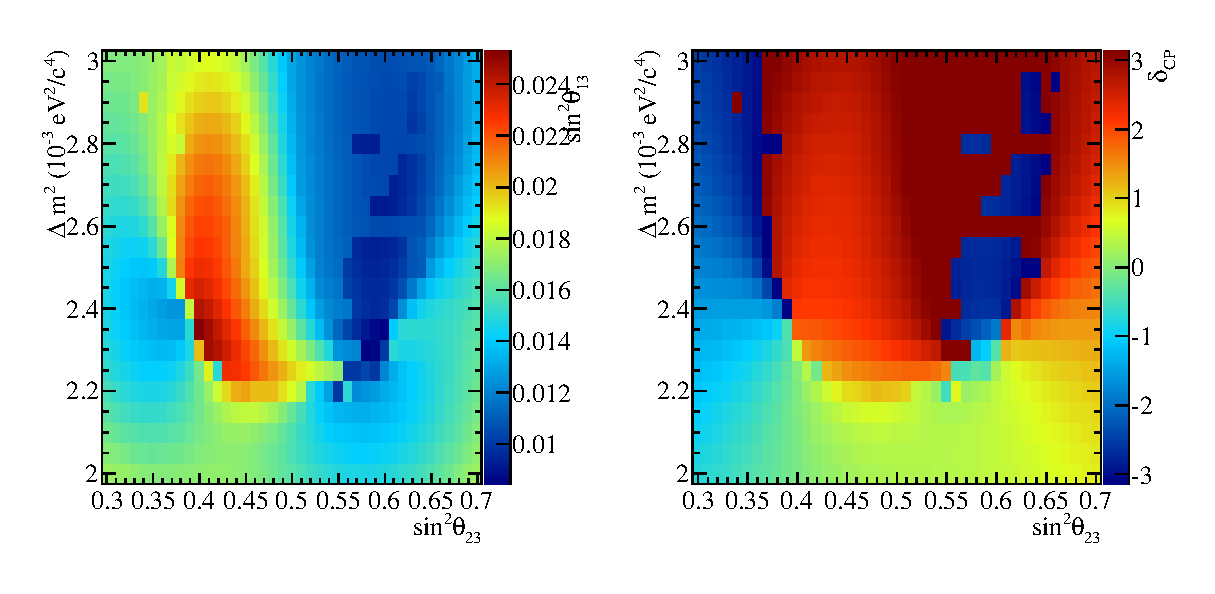
\includegraphics[width=10cm]{./images/validation/toy_dataset1_theta23_dmsq_extra.eps}
\caption {
 Best fit value of $sin^{2}\theta_{13}$ and $\delta_{CP}$
for the fit in the ($|\Delta m^{2}|$,$sin^{2}\theta_{23}$) space
for fake dataset \#1.
}
\end{minipage}
\end{center}

\vfill
\vspace*{0.5cm}
\begin{center}
\begin{minipage}[t]{0.48\linewidth}

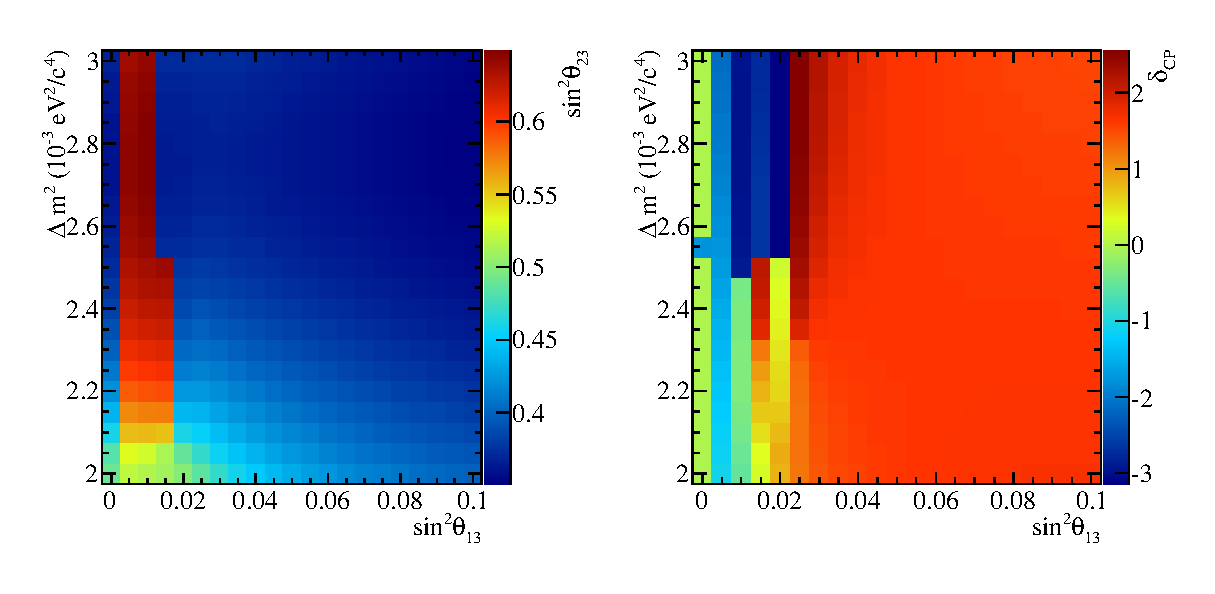
\includegraphics[width=10cm]{./images/validation/toy_dataset1_theta13_dmsq_extra.eps}
\caption {
 Best fit value of $sin^{2}\theta_{23}$ and $\delta_{CP}$
for the fit in the ($|\Delta m^{2}|$,$sin^{2}\theta_{13}$) space
for fake dataset \#1.
}
\end{minipage}
\end{center}

\vfill
\vspace*{0.5cm}
\begin{center}
\begin{minipage}[t]{0.48\linewidth}

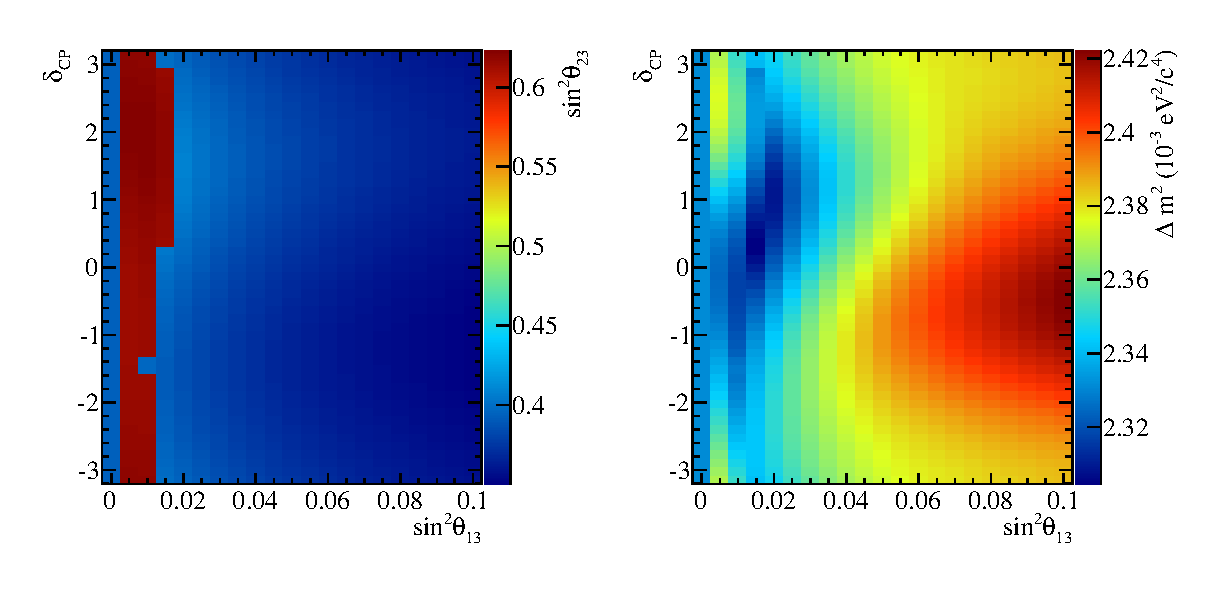
\includegraphics[width=10cm]{./images/validation/toy_dataset1_theta13_deltacp_extra.eps}
\caption {
 Best fit value of $sin^{2}\theta_{23}$ and $|\Delta m^{2}|$ 
for the fit in the ($\delta_{CP}$,$sin^{2}\theta_{23}$) space
for fake dataset \#1.
}
\end{minipage}
\end{center}

\vfill
\vspace*{0.5cm}
\begin{center}
\begin{minipage}[t]{0.48\linewidth}

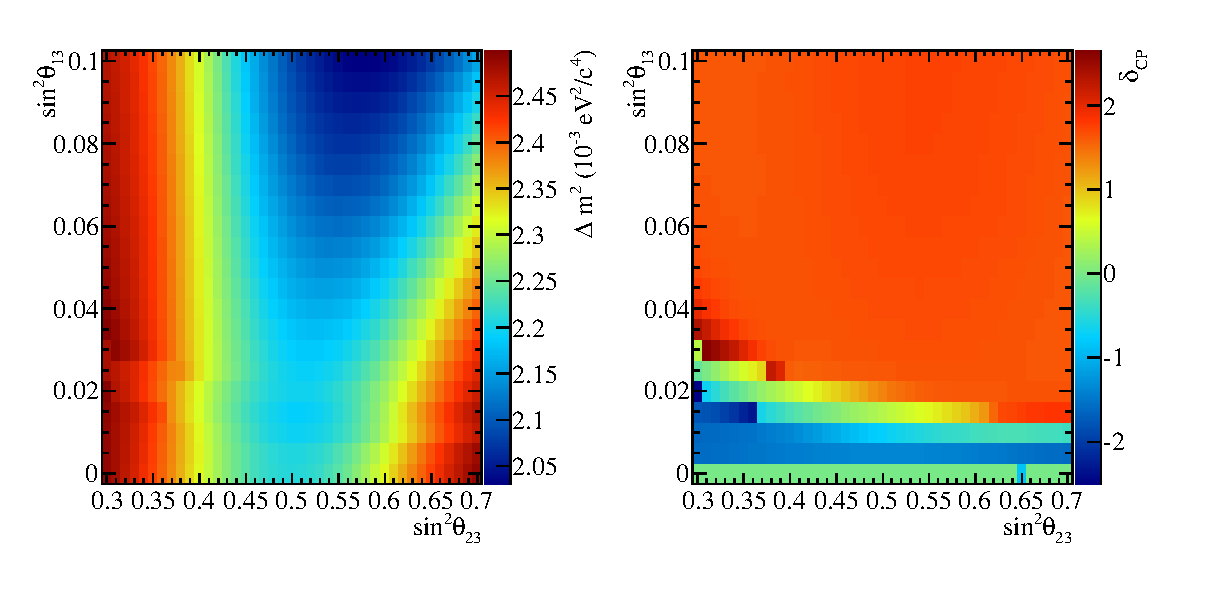
\includegraphics[width=10cm]{./images/validation/toy_dataset1_theta13_theta23_extra.eps}
\caption {
 Best fit value of $\delta_{CP}$ and $|\Delta m^{2}|$ 
for the fit in the ($sin^{2}\theta_{23}$,$sin^{2}\theta_{13}$) space
for fake dataset \#1.
}
\end{minipage}
\end{center}

\label{fig:validation:toys:extra_toy1}
\end{figure*}


% 
% 
% ..............................................
% Fake dataset #2
% 
%
\clearpage

\begin{figure*}[htb]

\begin{center}
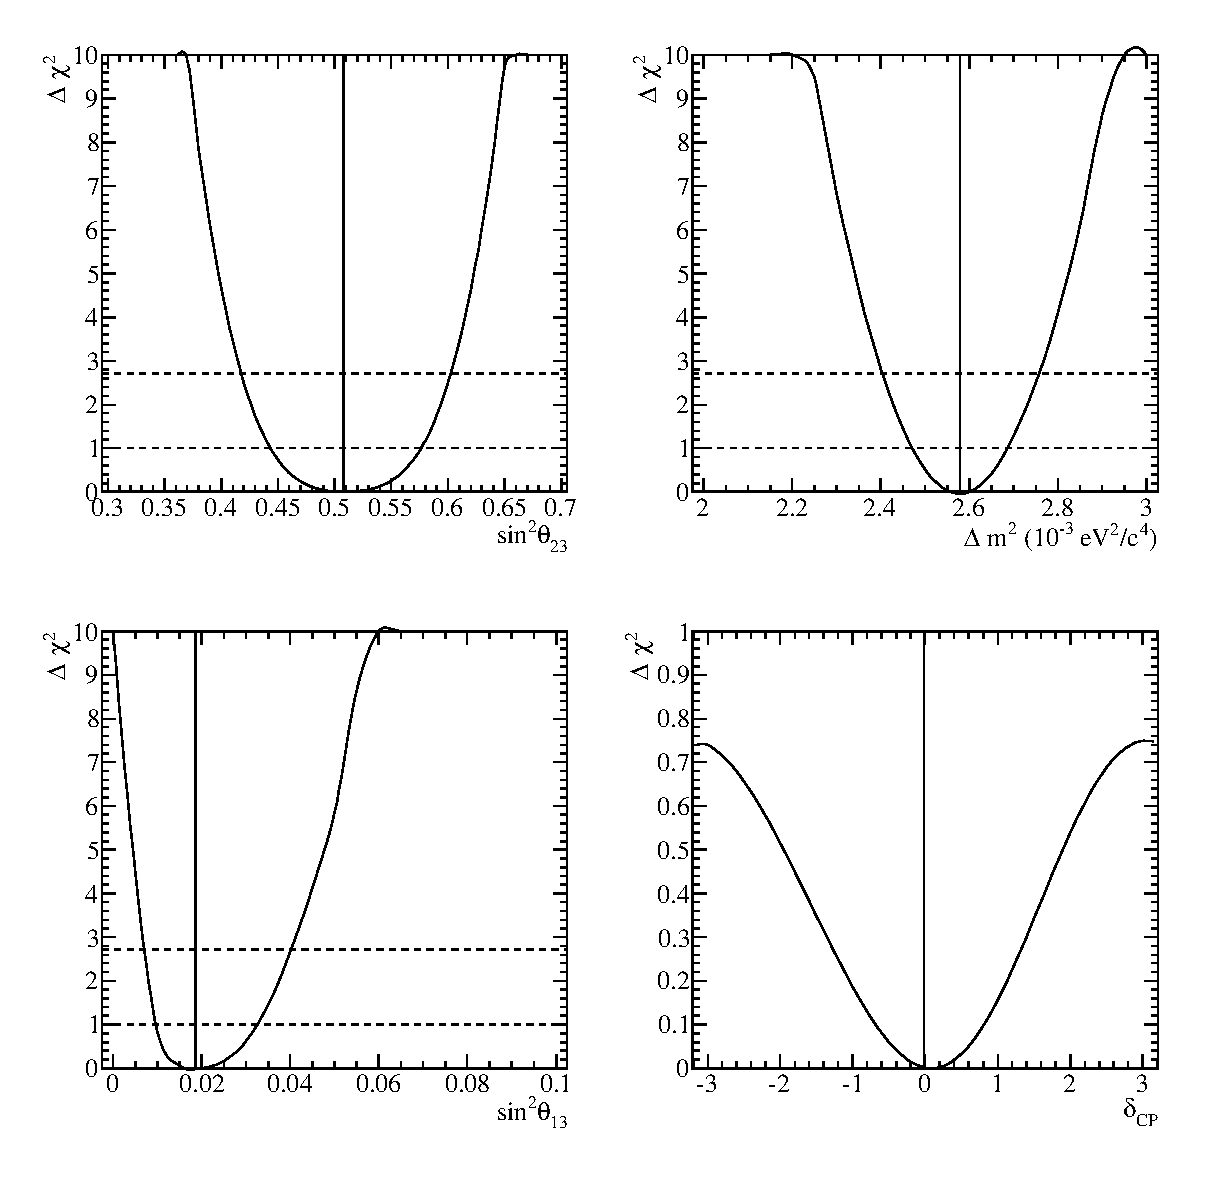
\includegraphics[width=25pc]{./images/validation/toy_dataset2_1D.eps}
\caption {
 $\Delta\chi^2$ as function of $\sin^{2}\theta_{23}$,$|\Delta m^{2}|$,$\sin^{2}\theta_{13}$ and $\delta_{CP}$
for fake dataset \#2.
  At each point, $\chi^2$ was minimized with respect to the oscillation parameters not shown in each figure
and all 64 systematic parameters.
}
\label{fig:validation:toys:1D_toy2}
\end{center}

\vfill
\vspace*{0.7cm}

\begin{center}
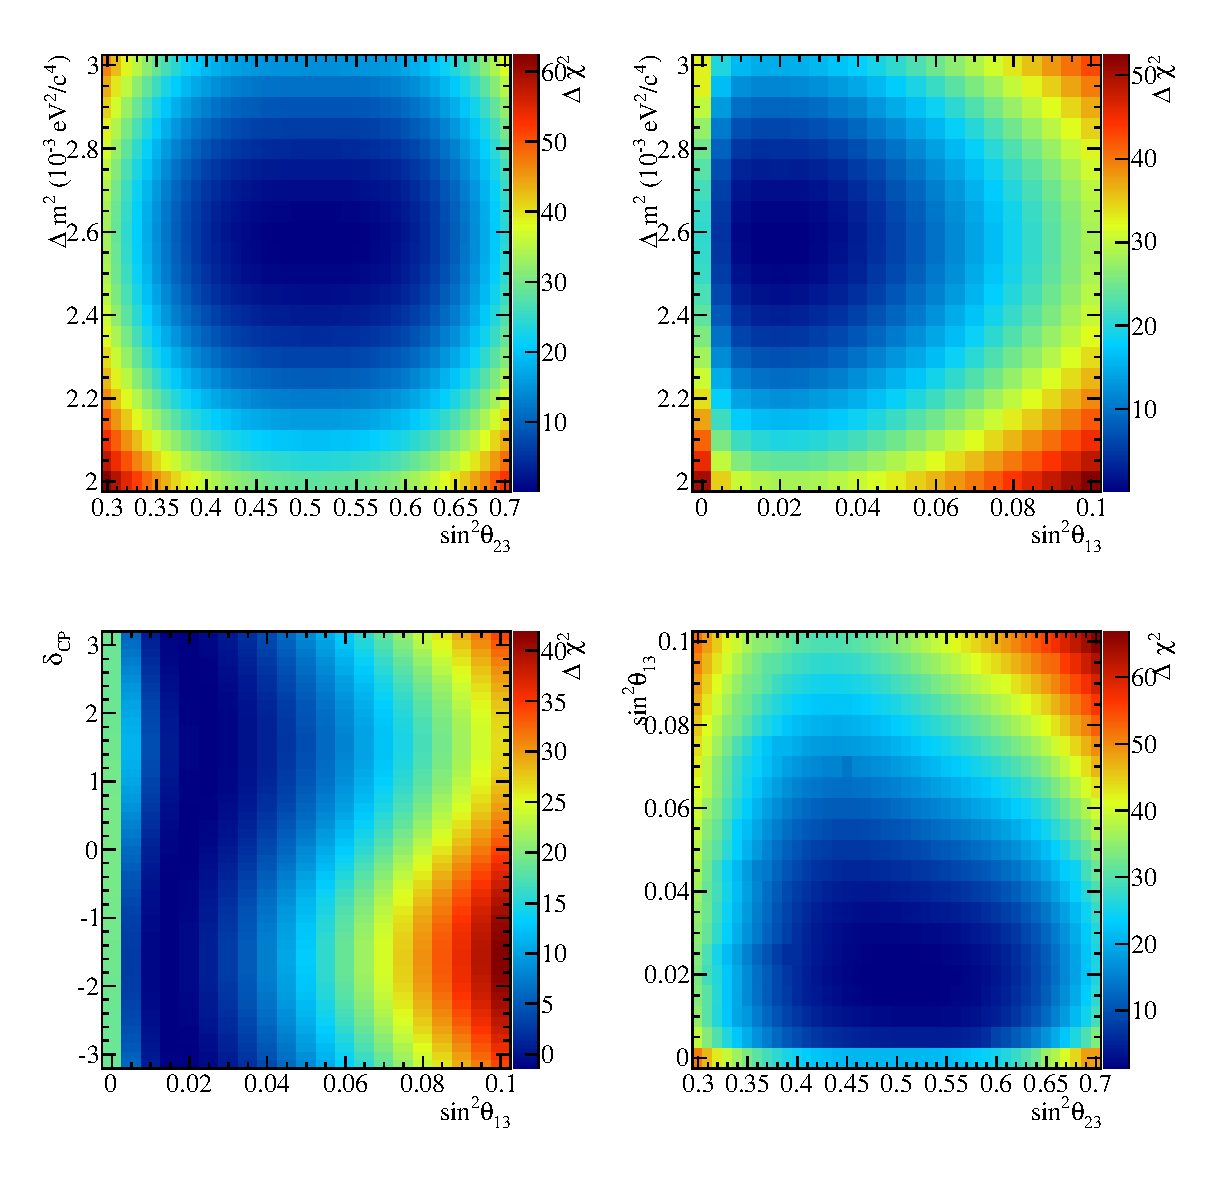
\includegraphics[width=30pc]{./images/validation/toy_dataset2_colz.eps}
\caption {
  $\Delta\chi^2$ surface in
($|\Delta m^{2}|$,$sin^{2}\theta_{23}$), 
($|\Delta m^{2}|$,$sin^{2}\theta_{13}$), 
($\delta_{CP}$,$sin^{2}\theta_{13}$) and 
($sin^{2}\theta_{13}$,$sin^{2}\theta_{23}$)
 spaces for fake dataset \#2.
At each point, $\chi^2$ was minimized with respect to the oscillation parameters not shown in each figure
and all 64 systematic parameters.
}
\label{fig:validation:toys:colz_toy2}
\end{center}

\end{figure*}


\begin{figure*}[htb]
\begin{center}
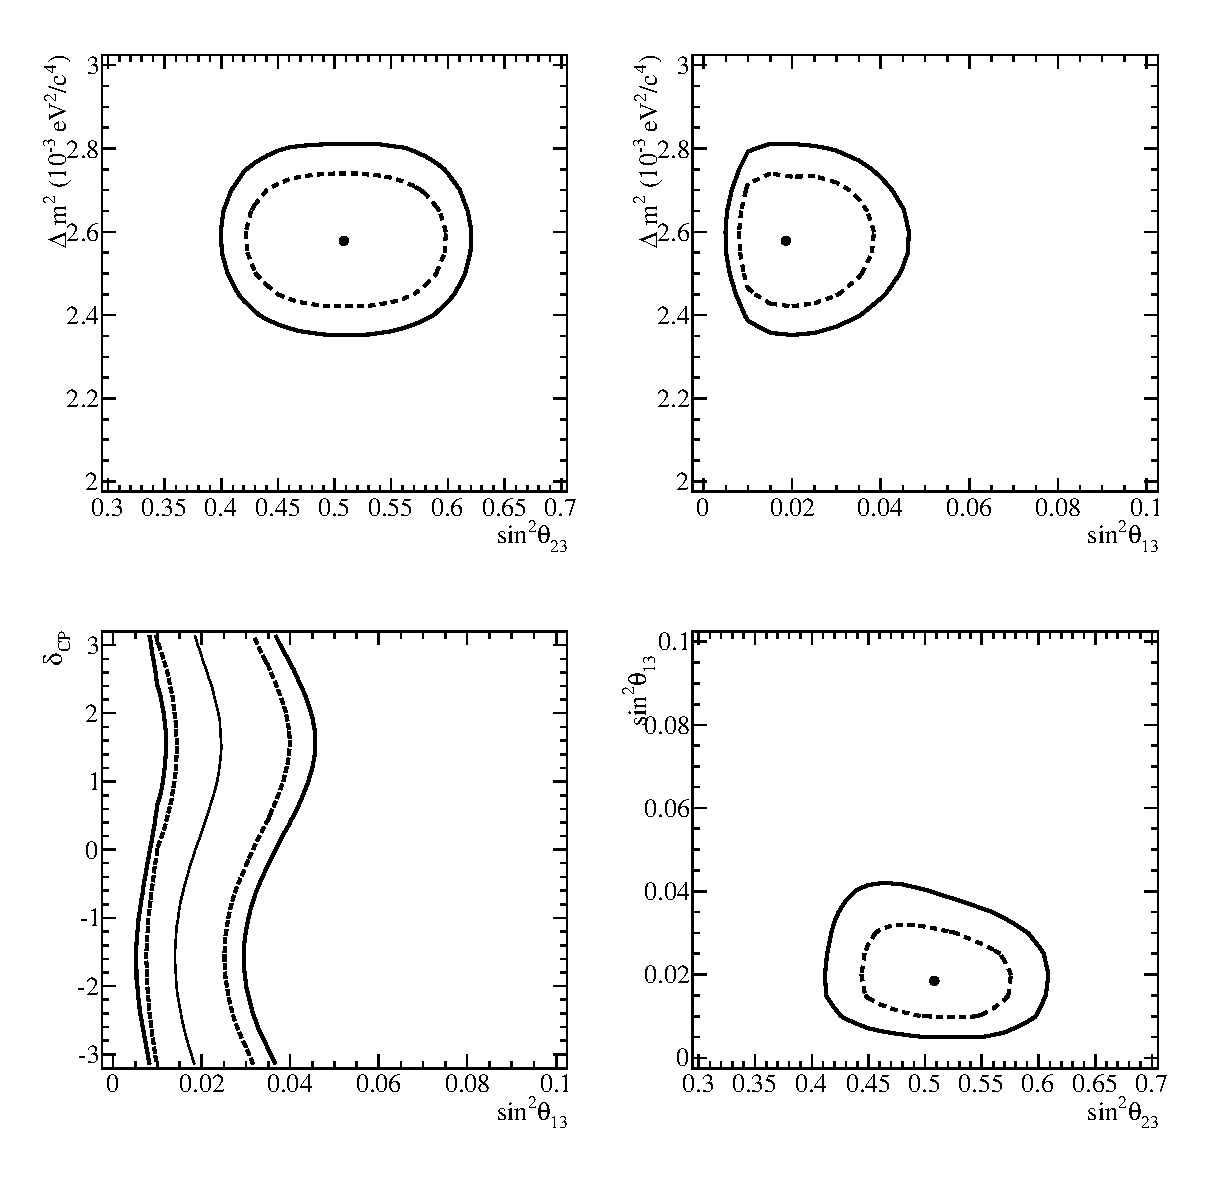
\includegraphics[width=40pc]{./images/validation/toy_dataset2_2D.eps}
\caption {
 68\% and 90\% CL regions in 
($|\Delta m^{2}|$,$sin^{2}\theta_{23}$), 
($|\Delta m^{2}|$,$sin^{2}\theta_{13}$), 
($\delta_{CP}$,$sin^{2}\theta_{13}$) and 
($sin^{2}\theta_{13}$,$sin^{2}\theta_{23}$)
 spaces for fake dataset \#2.
At each point, $\chi^2$ was minimized with respect to the oscillation parameters not shown in each figure
and all 64 systematic parameters.
}
\label{fig:validation:toys:2D_toy2}
\end{center}
\end{figure*}


\begin{figure*}[htb]
\begin{center}
\begin{minipage}[t]{0.48\linewidth}

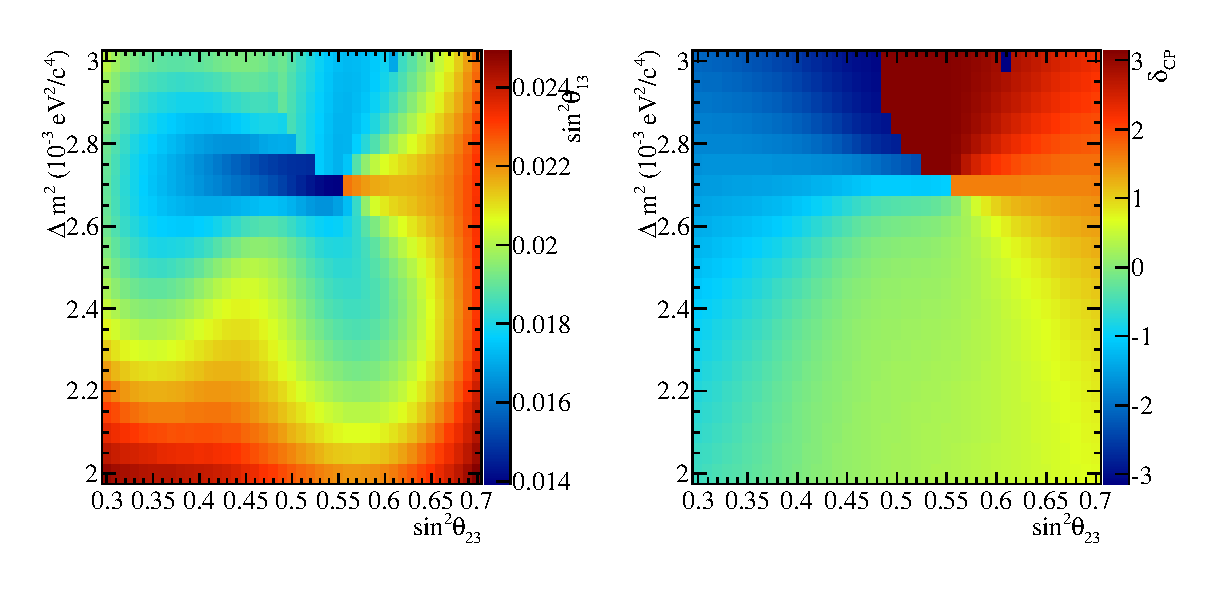
\includegraphics[width=10cm]{./images/validation/toy_dataset2_theta23_dmsq_extra.eps}
\caption {
 Best fit value of $sin^{2}\theta_{13}$ and $\delta_{CP}$
for the fit in the ($|\Delta m^{2}|$,$sin^{2}\theta_{23}$) space
for fake dataset \#2.
}
\end{minipage}
\end{center}

\vfill
\vspace*{0.5cm}
\begin{center}
\begin{minipage}[t]{0.48\linewidth}

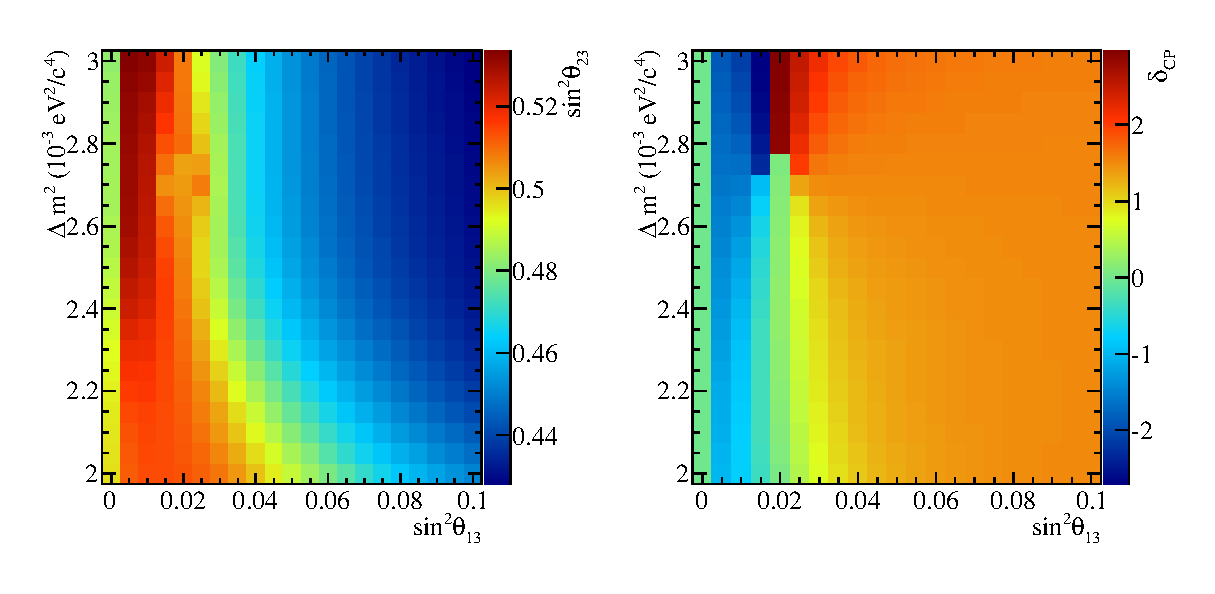
\includegraphics[width=10cm]{./images/validation/toy_dataset2_theta13_dmsq_extra.eps}
\caption {
 Best fit value of $sin^{2}\theta_{23}$ and $\delta_{CP}$
for the fit in the ($|\Delta m^{2}|$,$sin^{2}\theta_{13}$) space
for fake dataset \#2.
}
\end{minipage}
\end{center}

\vfill
\vspace*{0.5cm}
\begin{center}
\begin{minipage}[t]{0.48\linewidth}

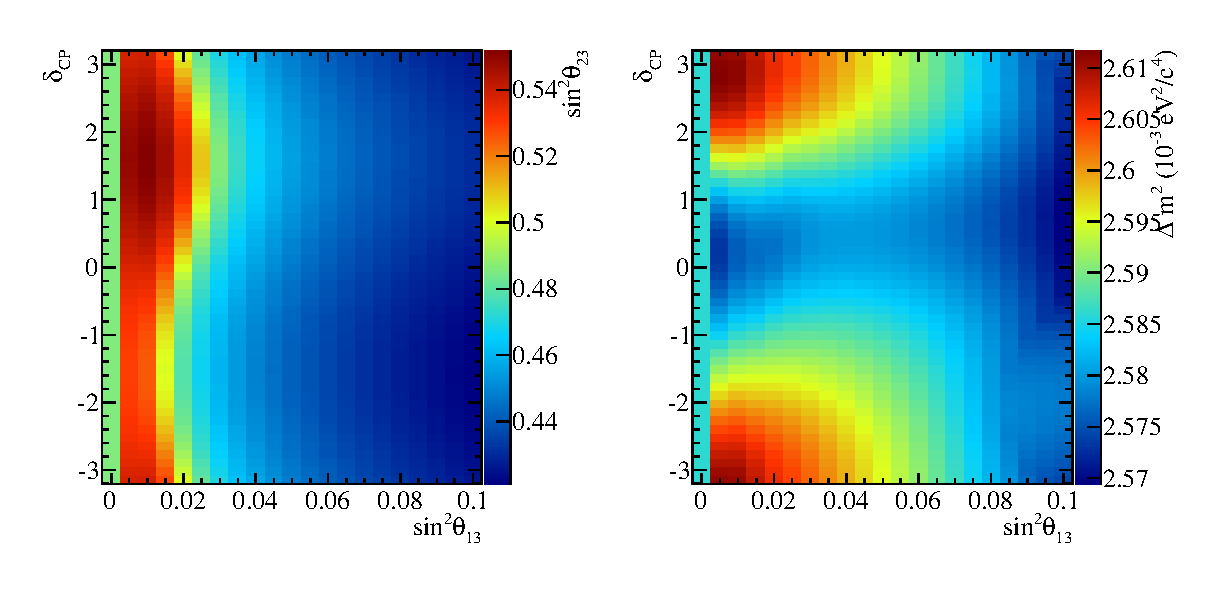
\includegraphics[width=10cm]{./images/validation/toy_dataset2_theta13_deltacp_extra.eps}
\caption {
 Best fit value of $sin^{2}\theta_{23}$ and $|\Delta m^{2}|$ 
for the fit in the ($\delta_{CP}$,$sin^{2}\theta_{23}$) space
for fake dataset \#2.
}

\end{minipage}
\end{center}
\vfill
\vspace*{0.5cm}
\begin{center}
\begin{minipage}[t]{0.48\linewidth}

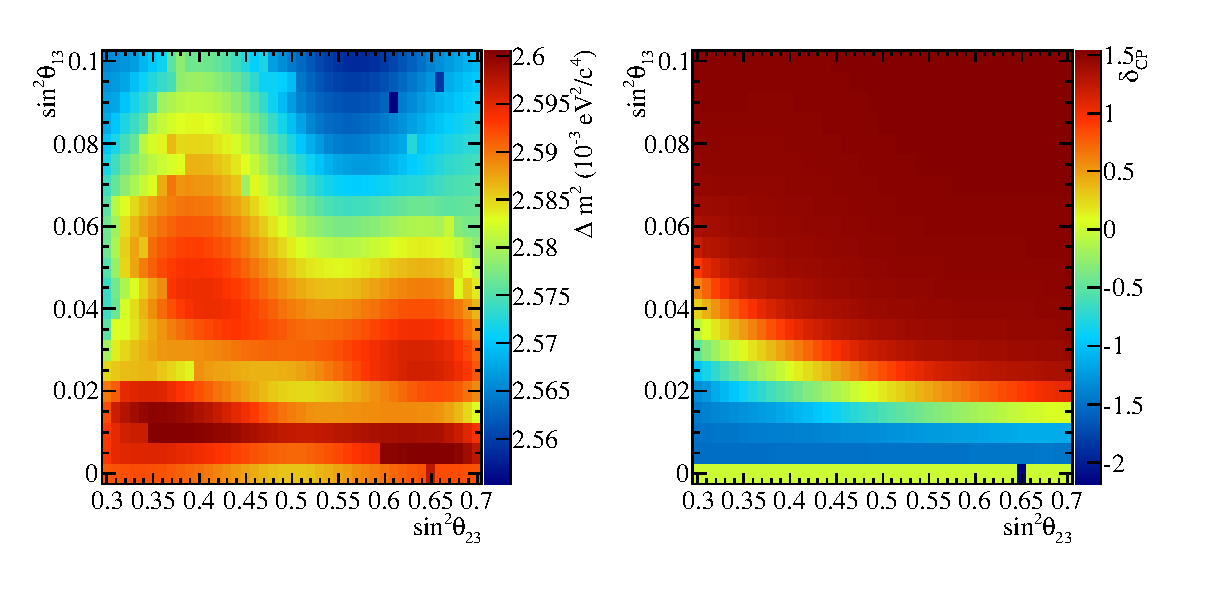
\includegraphics[width=10cm]{./images/validation/toy_dataset2_theta13_theta23_extra.eps}
\caption {
 Best fit value of $\delta_{CP}$ and $|\Delta m^{2}|$ 
for the fit in the ($sin^{2}\theta_{23}$,$sin^{2}\theta_{13}$) space
for fake dataset \#2.
}
\end{minipage}
\end{center}

\label{fig:validation:toys:extra_toy2}
\end{figure*}


% 
% 
% ..............................................
% Fake dataset #3
% 
%
\clearpage

\begin{figure*}[htb]

\begin{center}
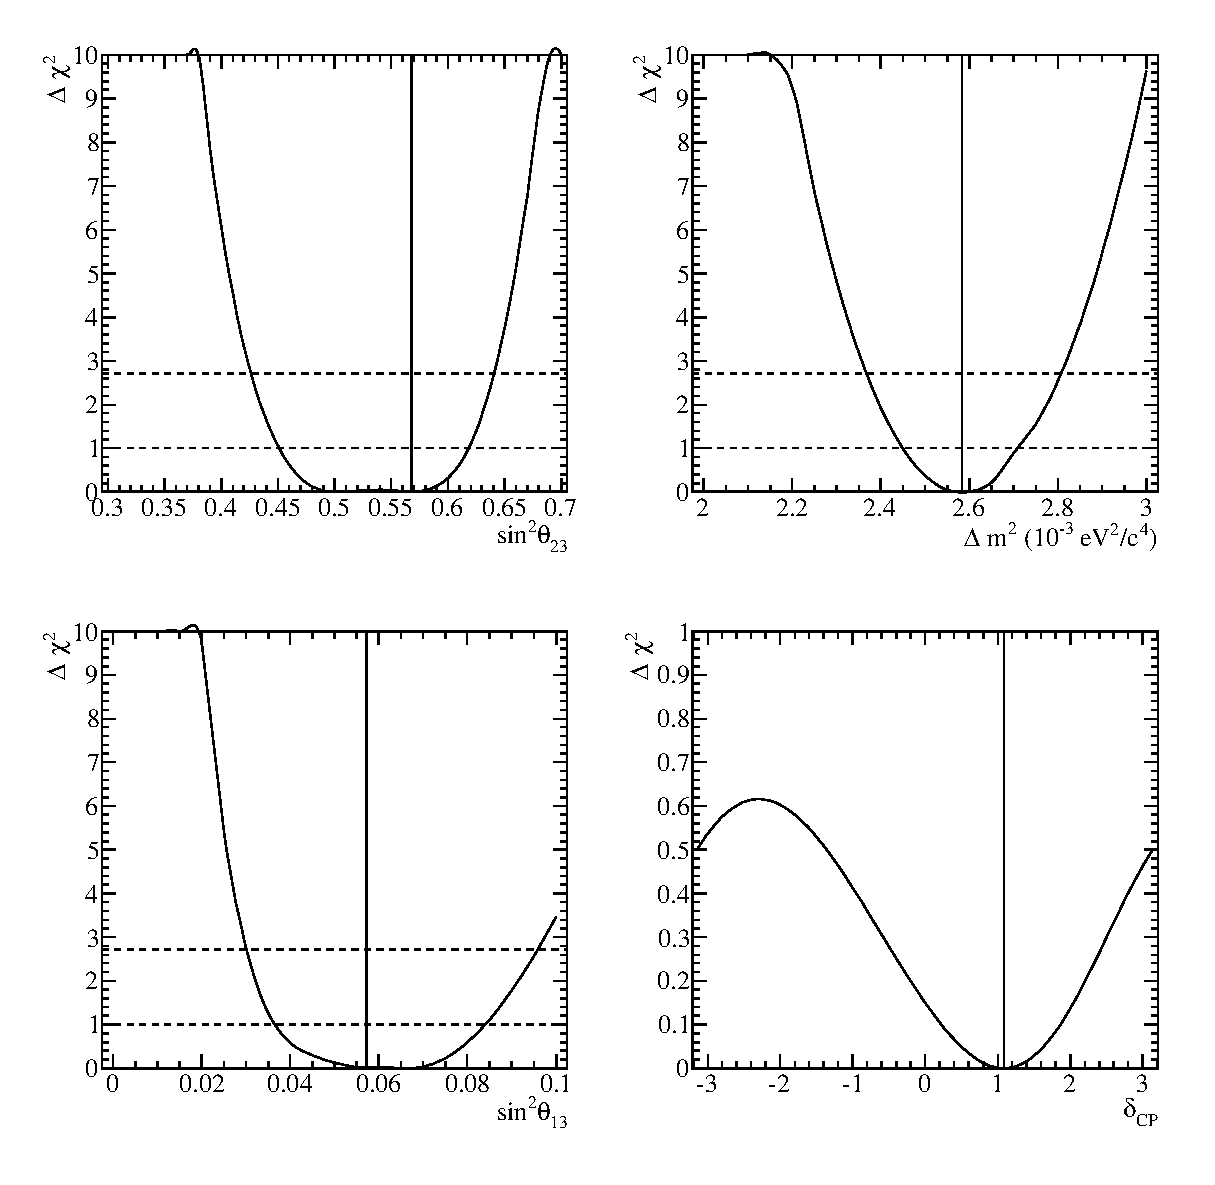
\includegraphics[width=25pc]{./images/validation/toy_dataset3_1D.eps}
\caption {
 $\Delta\chi^2$ as function of $\sin^{2}\theta_{23}$,$|\Delta m^{2}|$,$\sin^{2}\theta_{13}$ and $\delta_{CP}$
for fake dataset \#3.
  At each point, $\chi^2$ was minimized with respect to the oscillation parameters not shown in each figure
and all 64 systematic parameters.
}
\label{fig:validation:toys:1D_toy3}
\end{center}

\vfill
\vspace*{0.7cm}

\begin{center}
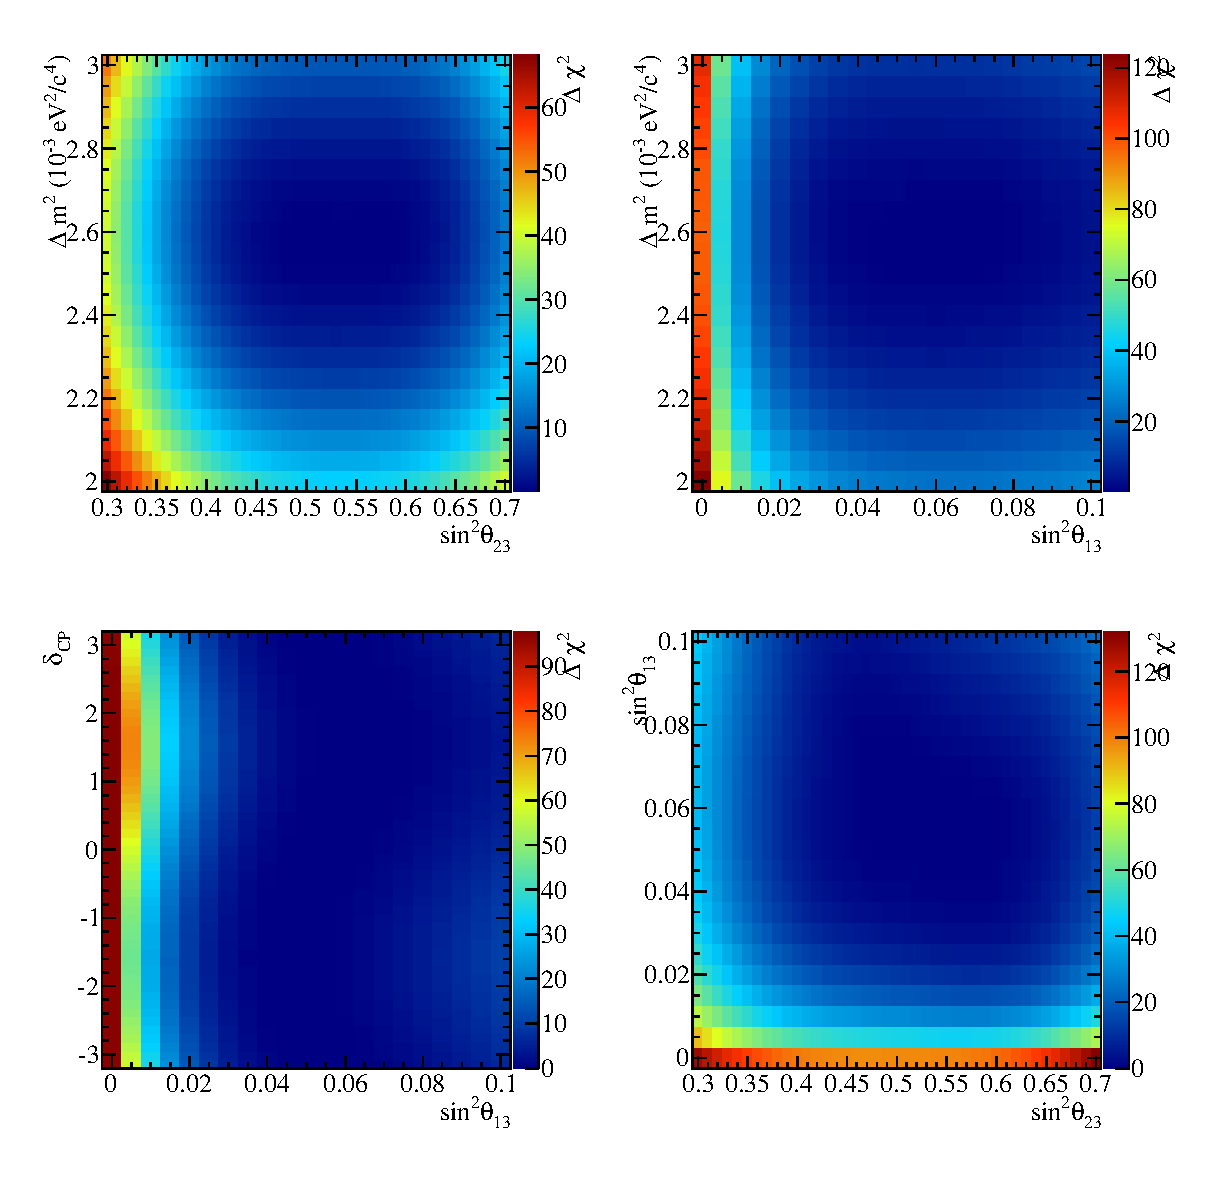
\includegraphics[width=30pc]{./images/validation/toy_dataset3_colz.eps}
\caption {
  $\Delta\chi^2$ surface in
($|\Delta m^{2}|$,$sin^{2}\theta_{23}$), 
($|\Delta m^{2}|$,$sin^{2}\theta_{13}$), 
($\delta_{CP}$,$sin^{2}\theta_{13}$) and 
($sin^{2}\theta_{13}$,$sin^{2}\theta_{23}$)
 spaces for fake dataset \#3.
At each point, $\chi^2$ was minimized with respect to the oscillation parameters not shown in each figure
and all 64 systematic parameters.
}
\label{fig:validation:toys:colz_toy3}
\end{center}

\end{figure*}


\begin{figure*}[htb]



\begin{center}
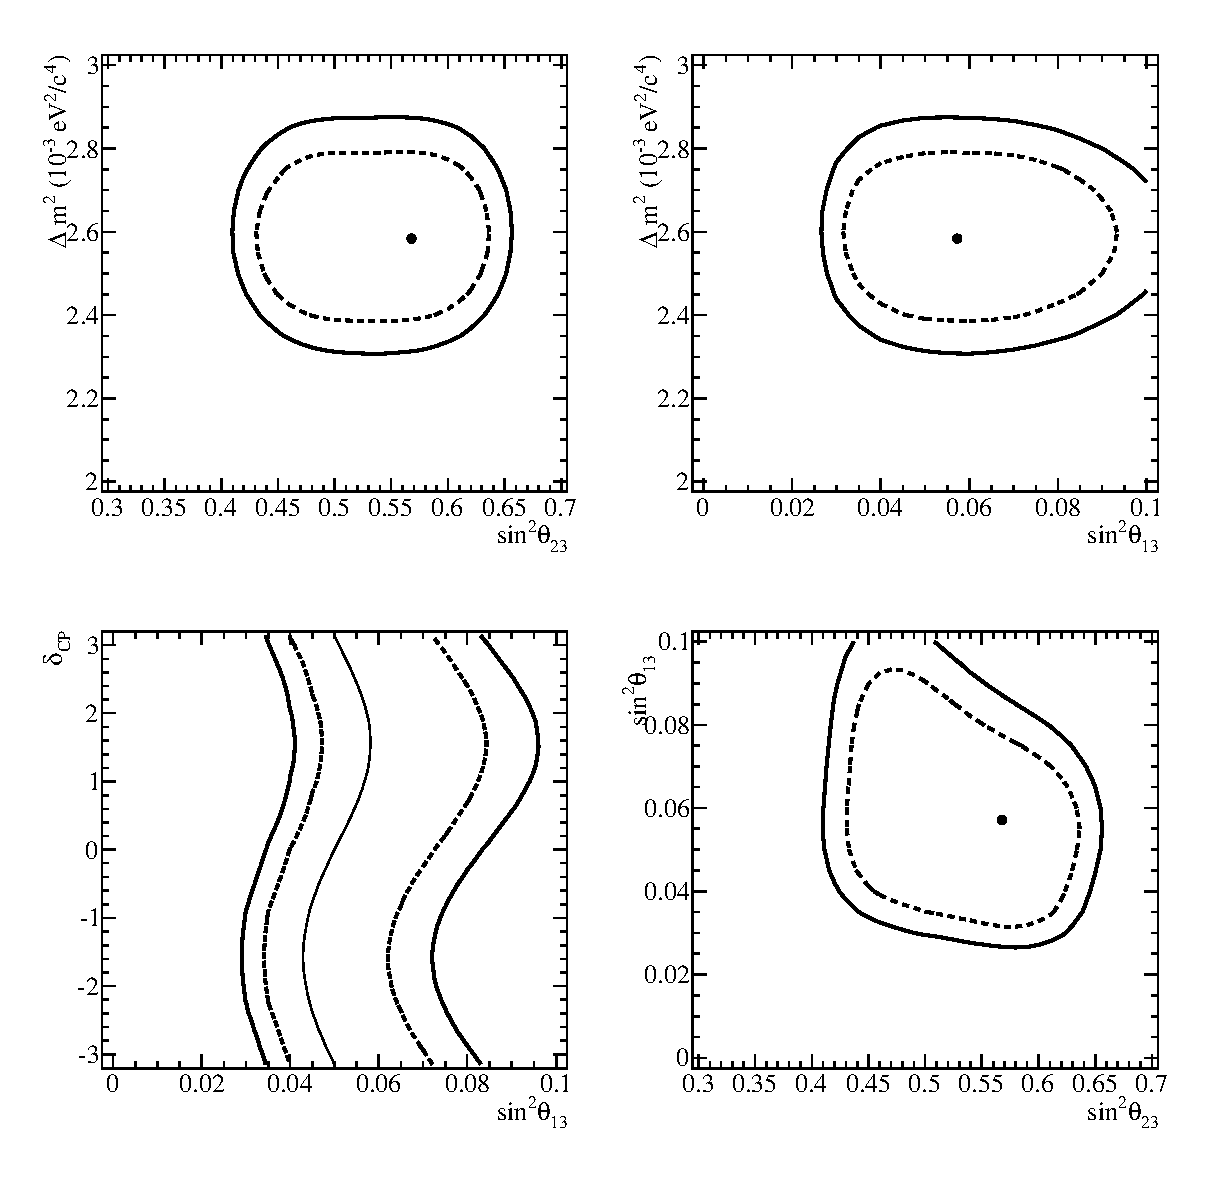
\includegraphics[width=40pc]{./images/validation/toy_dataset3_2D.eps}
\caption {
 68\% and 90\% CL regions in 
($|\Delta m^{2}|$,$sin^{2}\theta_{23}$), 
($|\Delta m^{2}|$,$sin^{2}\theta_{13}$), 
($\delta_{CP}$,$sin^{2}\theta_{13}$) and 
($sin^{2}\theta_{13}$,$sin^{2}\theta_{23}$)
 spaces for fake dataset \#3.
At each point, $\chi^2$ was minimized with respect to the oscillation parameters not shown in each figure
and all 64 systematic parameters.
}
\label{fig:validation:toys:2D_toy3}
\end{center}
\end{figure*}


\begin{figure*}[htb]
\begin{center}
\begin{minipage}[t]{0.48\linewidth}

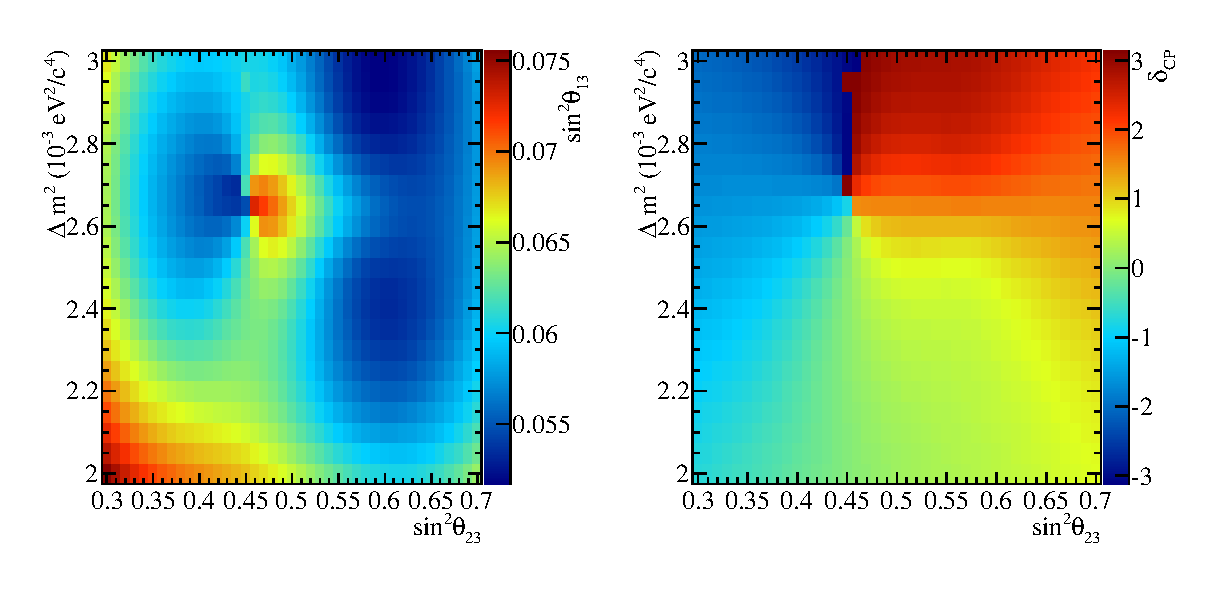
\includegraphics[width=10cm]{./images/validation/toy_dataset3_theta23_dmsq_extra.eps}
\caption {
 Best fit value of $sin^{2}\theta_{13}$ and $\delta_{CP}$
for the fit in the ($|\Delta m^{2}|$,$sin^{2}\theta_{23}$) space
for fake dataset \#3.
}
\end{minipage}
\end{center}

\vfill
\vspace*{0.5cm}
\begin{center}
\begin{minipage}[t]{0.48\linewidth}

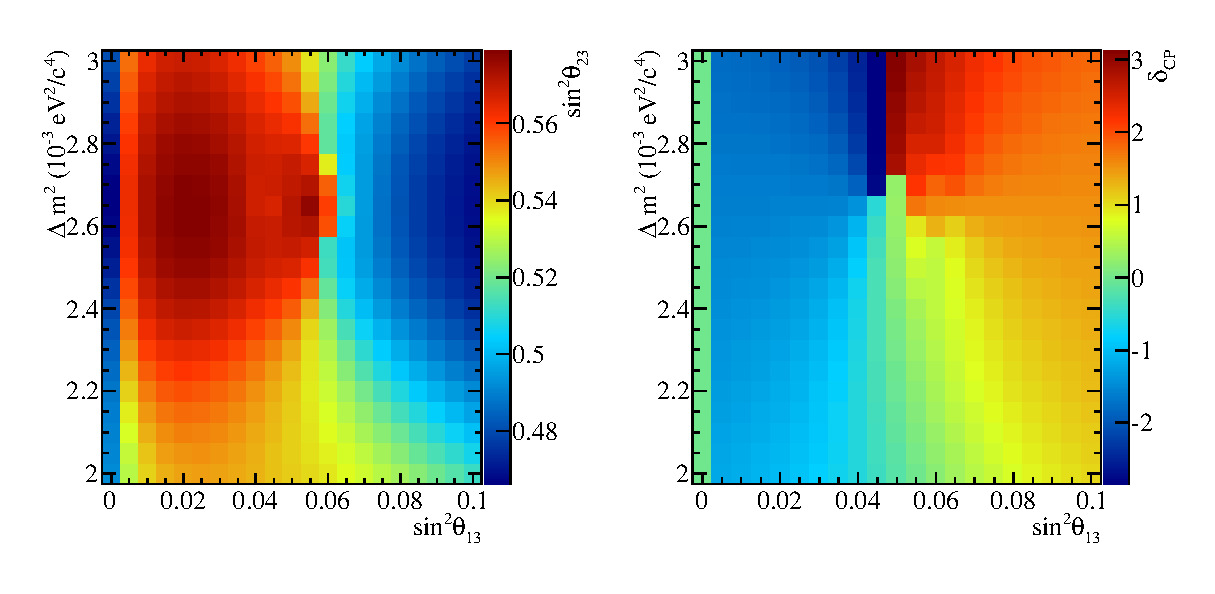
\includegraphics[width=10cm]{./images/validation/toy_dataset3_theta13_dmsq_extra.eps}
\caption {
 Best fit value of $sin^{2}\theta_{23}$ and $\delta_{CP}$
for the fit in the ($|\Delta m^{2}|$,$sin^{2}\theta_{13}$) space
for fake dataset \#3.
}
\end{minipage}
\end{center}

\vfill
\vspace*{0.5cm}
\begin{center}
\begin{minipage}[t]{0.48\linewidth}

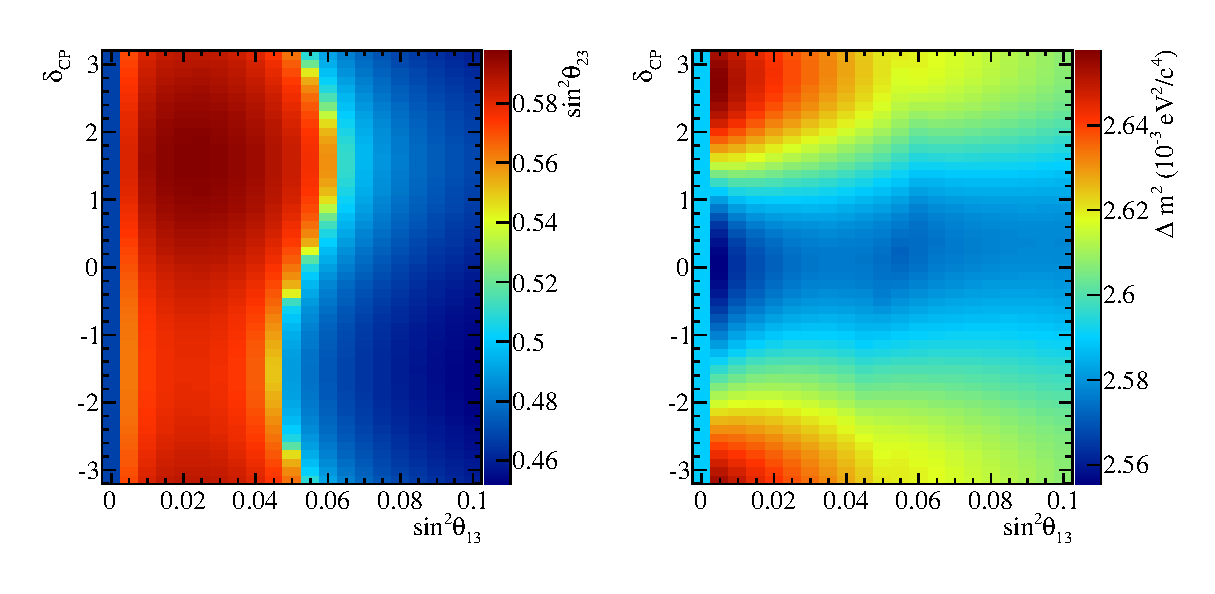
\includegraphics[width=10cm]{./images/validation/toy_dataset3_theta13_deltacp_extra.eps}
\caption {
 Best fit value of $sin^{2}\theta_{23}$ and $|\Delta m^{2}|$ 
for the fit in the ($\delta_{CP}$,$sin^{2}\theta_{23}$) space
for fake dataset \#3.
}
\end{minipage}
\end{center}

\vfill
\vspace*{0.5cm}
\begin{center}
\begin{minipage}[t]{0.48\linewidth}

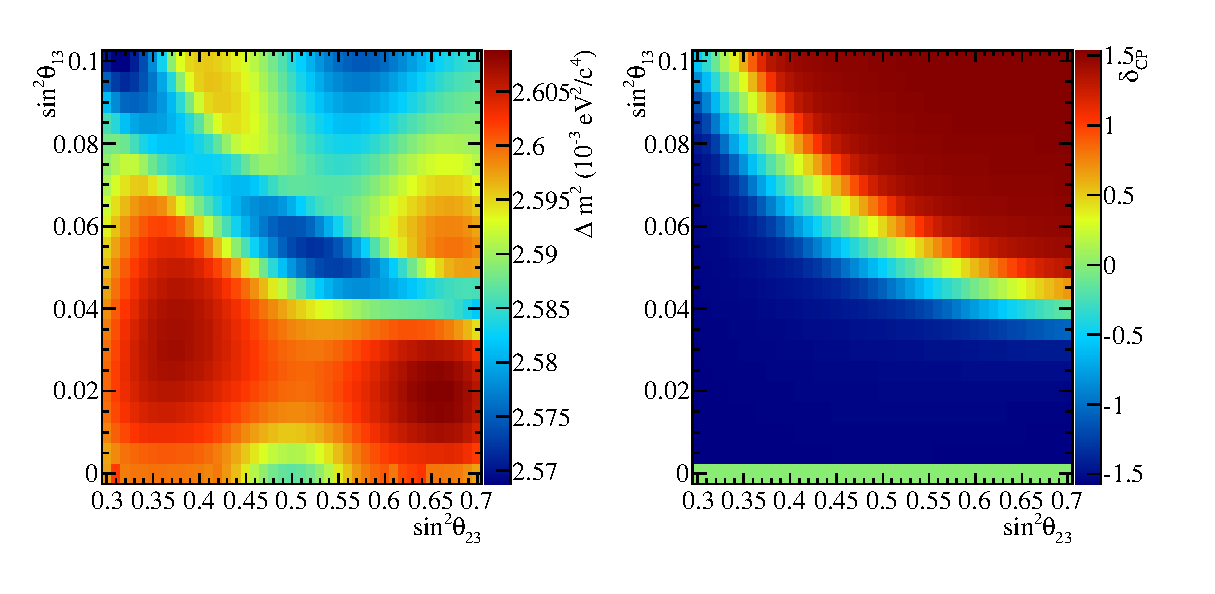
\includegraphics[width=10cm]{./images/validation/toy_dataset3_theta13_theta23_extra.eps}
\caption {
 Best fit value of $\delta_{CP}$ and $|\Delta m^{2}|$ 
for the fit in the ($sin^{2}\theta_{23}$,$sin^{2}\theta_{13}$) space
for fake dataset \#3.
}
\end{minipage}
\end{center}

\label{fig:validation:toys:extra_toy3}
\end{figure*}


% 
% 
% ..............................................
% Fake dataset #4
% 
%
\clearpage

\begin{figure*}[htb]

\begin{center}
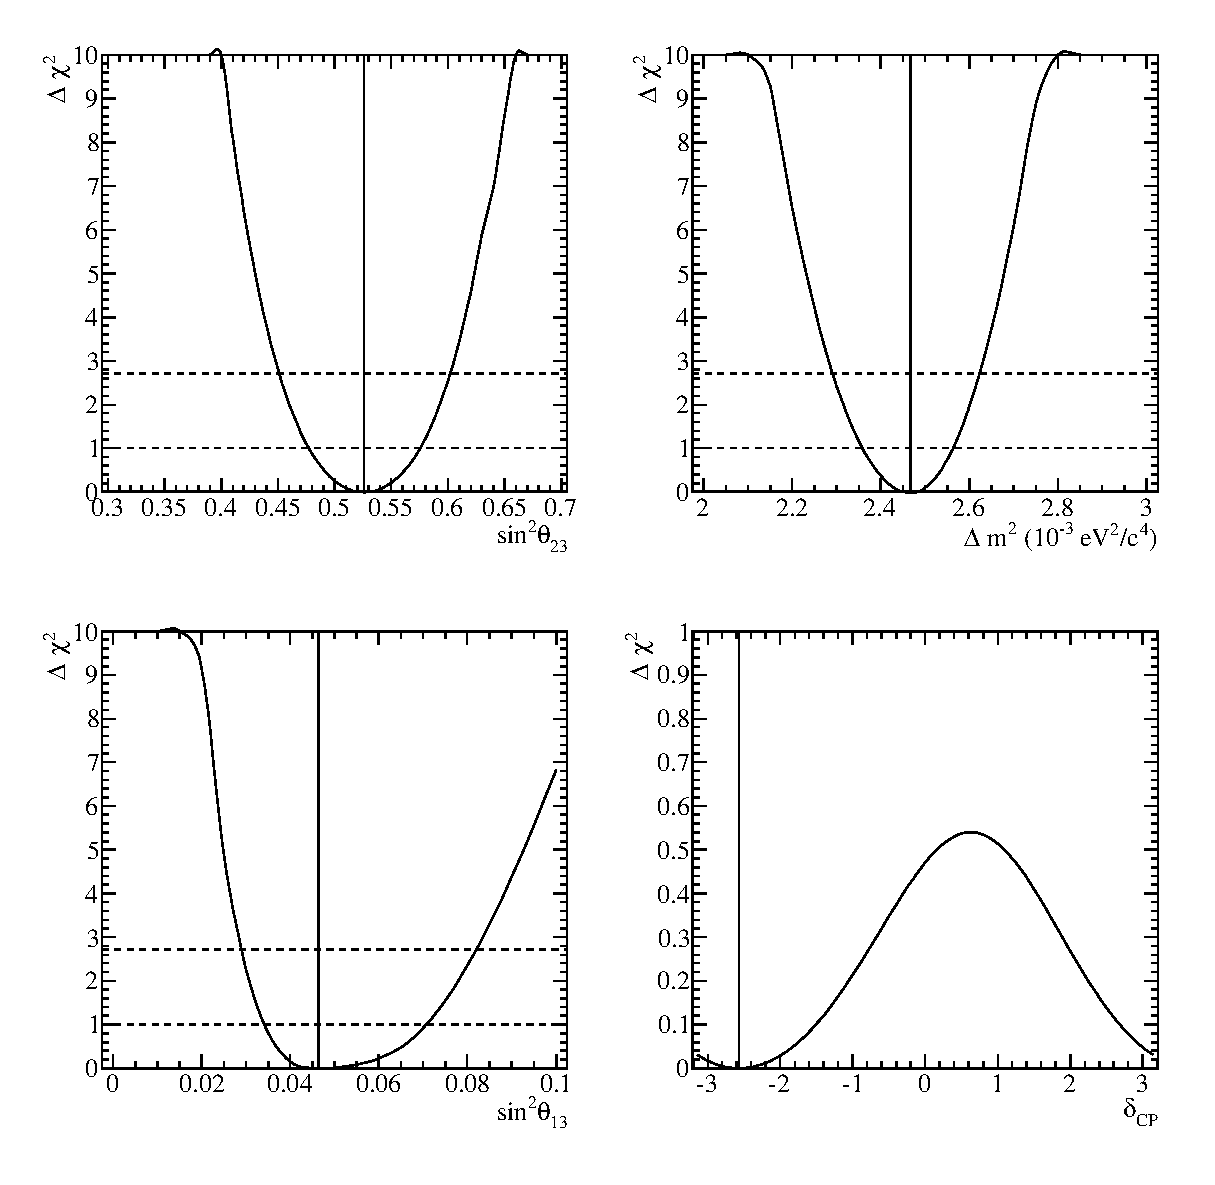
\includegraphics[width=25pc]{./images/validation/toy_dataset4_1D.eps}
\caption {
 $\Delta\chi^2$ as function of $\sin^{2}\theta_{23}$,$|\Delta m^{2}|$,$\sin^{2}\theta_{13}$ and $\delta_{CP}$
for fake dataset \#4.
  At each point, $\chi^2$ was minimized with respect to the oscillation parameters not shown in each figure
and all 64 systematic parameters.
}
\label{fig:validation:toys:1D_toy4}
\end{center}

\vfill
\vspace*{0.7cm}

\begin{center}
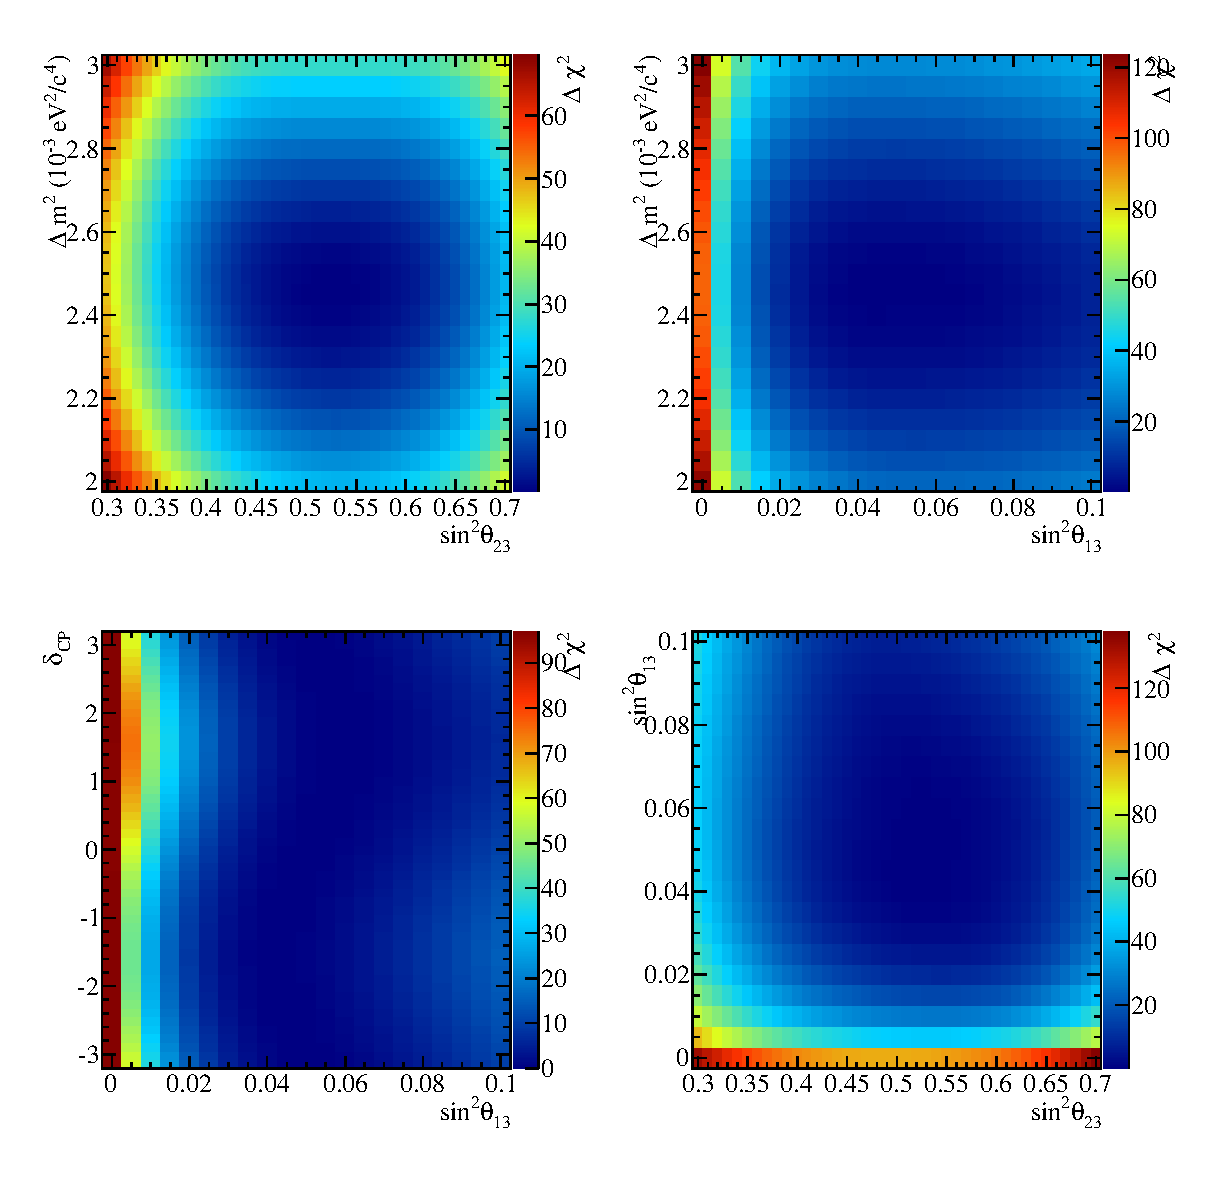
\includegraphics[width=30pc]{./images/validation/toy_dataset4_colz.eps}
\caption {
  $\Delta\chi^2$ surface in
($|\Delta m^{2}|$,$sin^{2}\theta_{23}$), 
($|\Delta m^{2}|$,$sin^{2}\theta_{13}$), 
($\delta_{CP}$,$sin^{2}\theta_{13}$) and 
($sin^{2}\theta_{13}$,$sin^{2}\theta_{23}$)
 spaces for fake dataset \#4.
At each point, $\chi^2$ was minimized with respect to the oscillation parameters not shown in each figure
and all 64 systematic parameters.
}
\label{fig:validation:toys:colz_toy4}
\end{center}


\end{figure*}


\begin{figure*}[htb]



\begin{center}
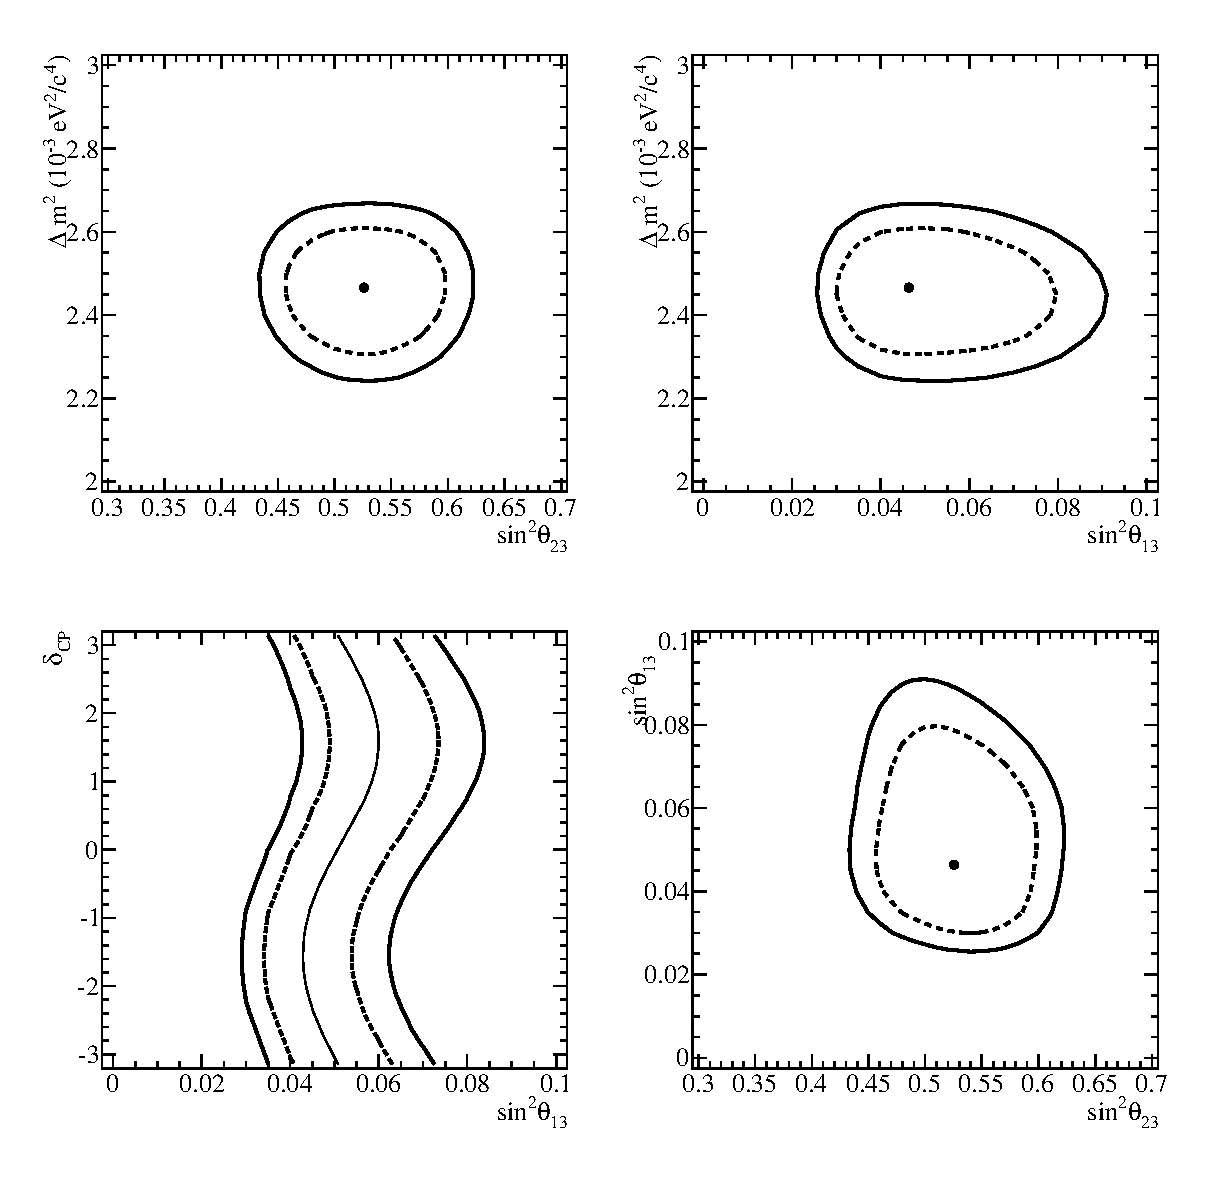
\includegraphics[width=40pc]{./images/validation/toy_dataset4_2D.eps}
\caption {
 68\% and 90\% CL regions in 
($|\Delta m^{2}|$,$sin^{2}\theta_{23}$), 
($|\Delta m^{2}|$,$sin^{2}\theta_{13}$), 
($\delta_{CP}$,$sin^{2}\theta_{13}$) and 
($sin^{2}\theta_{13}$,$sin^{2}\theta_{23}$)
 spaces for fake dataset \#4.
At each point, $\chi^2$ was minimized with respect to the oscillation parameters not shown in each figure
and all 64 systematic parameters.
}
\label{fig:validation:toys:2D_toy4}
\end{center}
\end{figure*}


\begin{figure*}[htb]
\begin{center}
\begin{minipage}[t]{0.48\linewidth}

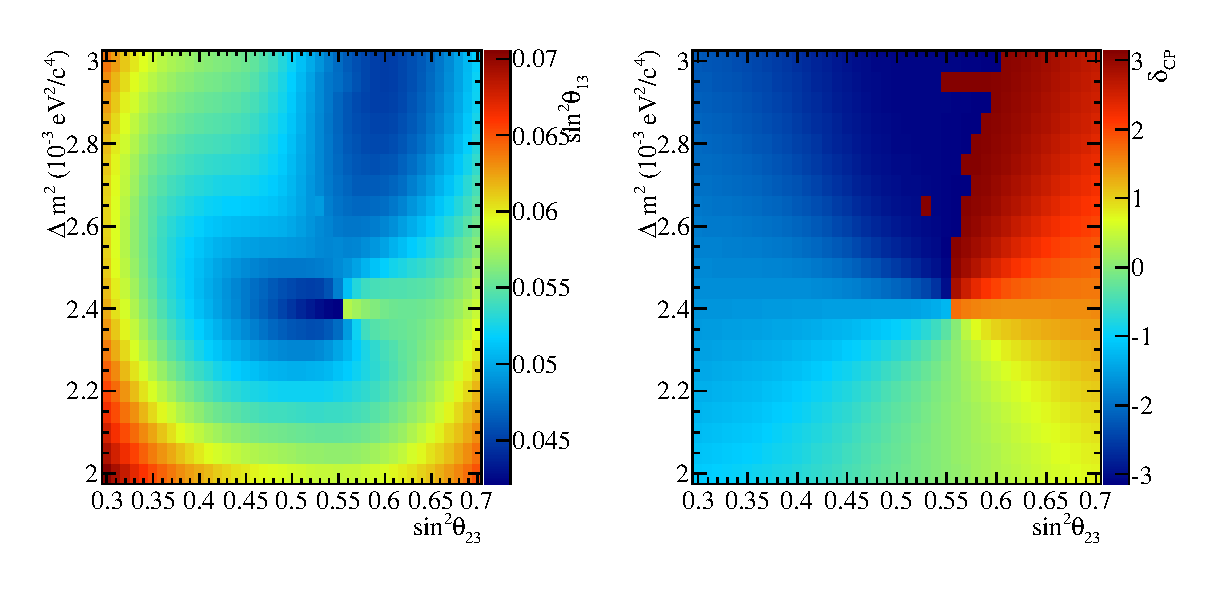
\includegraphics[width=10cm]{./images/validation/toy_dataset4_theta23_dmsq_extra.eps}
\caption {
 Best fit value of $sin^{2}\theta_{13}$ and $\delta_{CP}$
for the fit in the ($|\Delta m^{2}|$,$sin^{2}\theta_{23}$) space
for fake dataset \#4.
}
\end{minipage}
\end{center}

\vfill
\vspace*{0.5cm}
\begin{center}
\begin{minipage}[t]{0.48\linewidth}

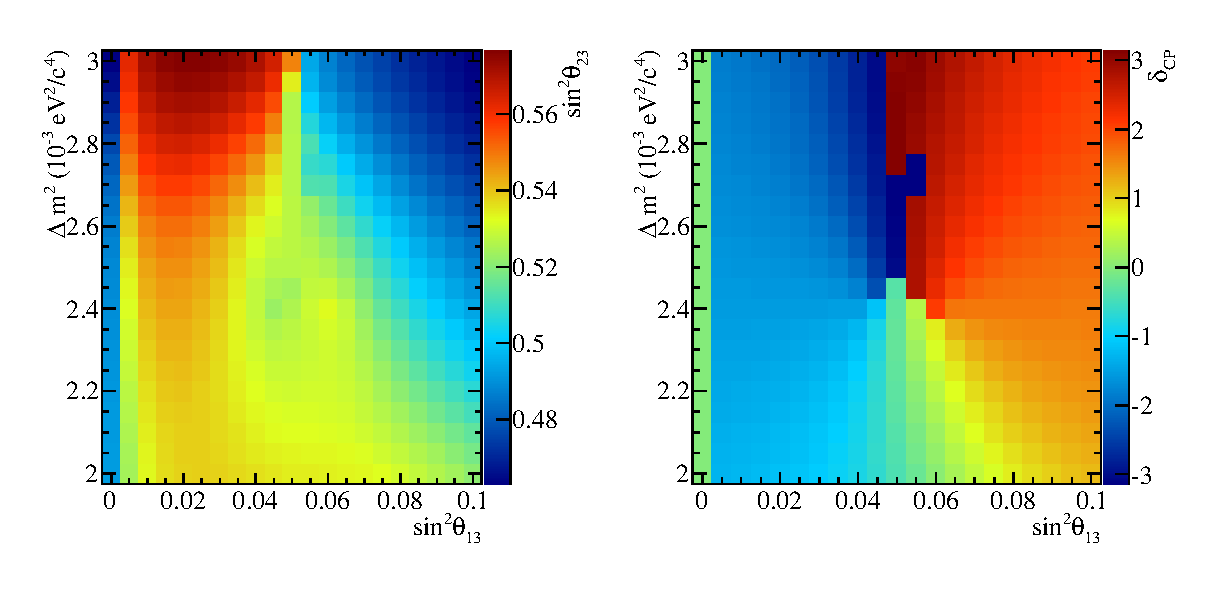
\includegraphics[width=10cm]{./images/validation/toy_dataset4_theta13_dmsq_extra.eps}
\caption {
 Best fit value of $sin^{2}\theta_{23}$ and $\delta_{CP}$
for the fit in the ($|\Delta m^{2}|$,$sin^{2}\theta_{13}$) space
for fake dataset \#4.
}
\end{minipage}
\end{center}

\vfill
\vspace*{0.5cm}
\begin{center}
\begin{minipage}[t]{0.48\linewidth}

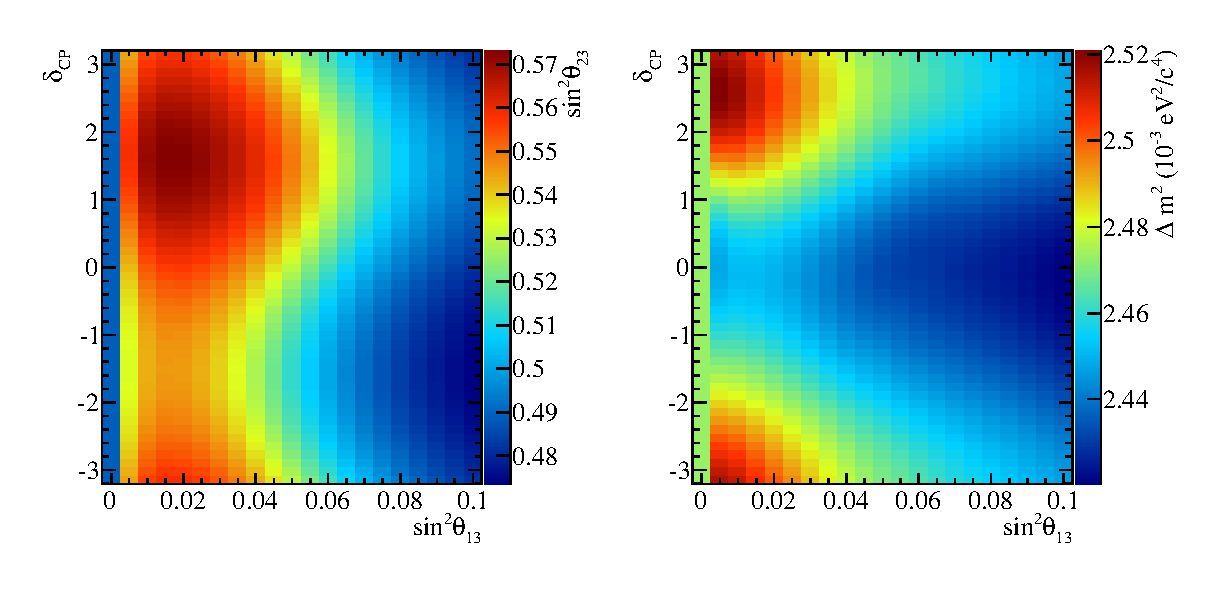
\includegraphics[width=10cm]{./images/validation/toy_dataset4_theta13_deltacp_extra.eps}
\caption {
 Best fit value of $sin^{2}\theta_{23}$ and $|\Delta m^{2}|$ 
for the fit in the ($\delta_{CP}$,$sin^{2}\theta_{23}$) space
for fake dataset \#4.
}
\end{minipage}
\end{center}

\vfill
\vspace*{0.5cm}
\begin{center}
\begin{minipage}[t]{0.48\linewidth}

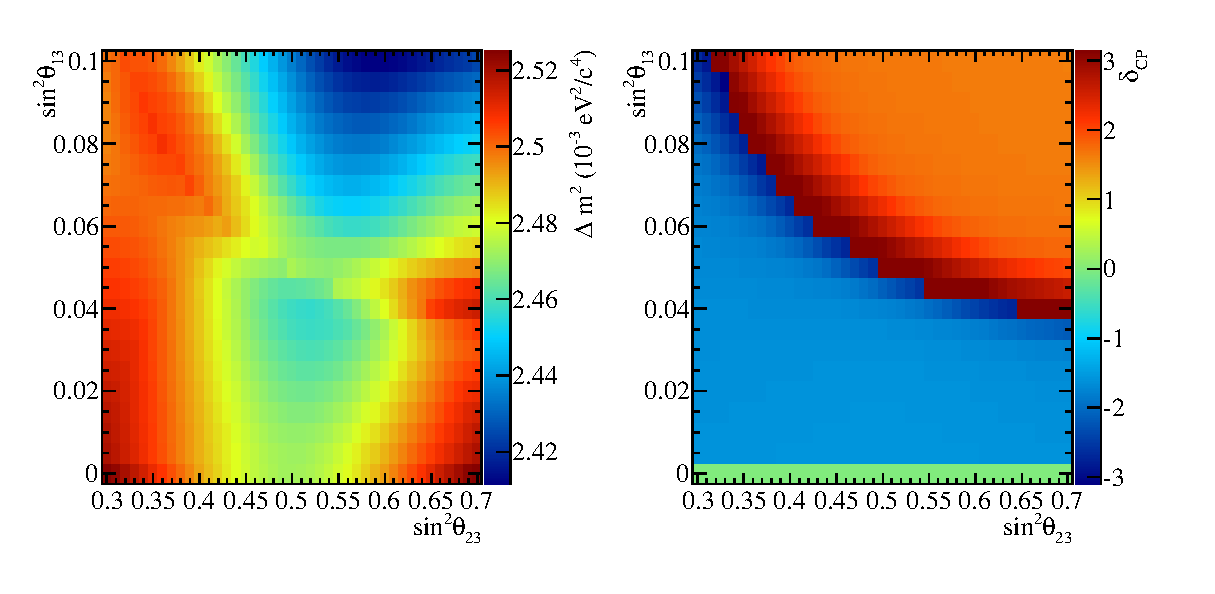
\includegraphics[width=10cm]{./images/validation/toy_dataset4_theta13_theta23_extra.eps}
\caption {
 Best fit value of $\delta_{CP}$ and $|\Delta m^{2}|$ 
for the fit in the ($sin^{2}\theta_{23}$,$sin^{2}\theta_{13}$) space
for fake dataset \#4.
}
\end{minipage}
\end{center}

\label{fig:validation:toys:extra_toy4}
\end{figure*}



% 
% 
% ..............................................
% Fake dataset #5
% 
%
\clearpage

\begin{figure*}[htb]

\begin{center}
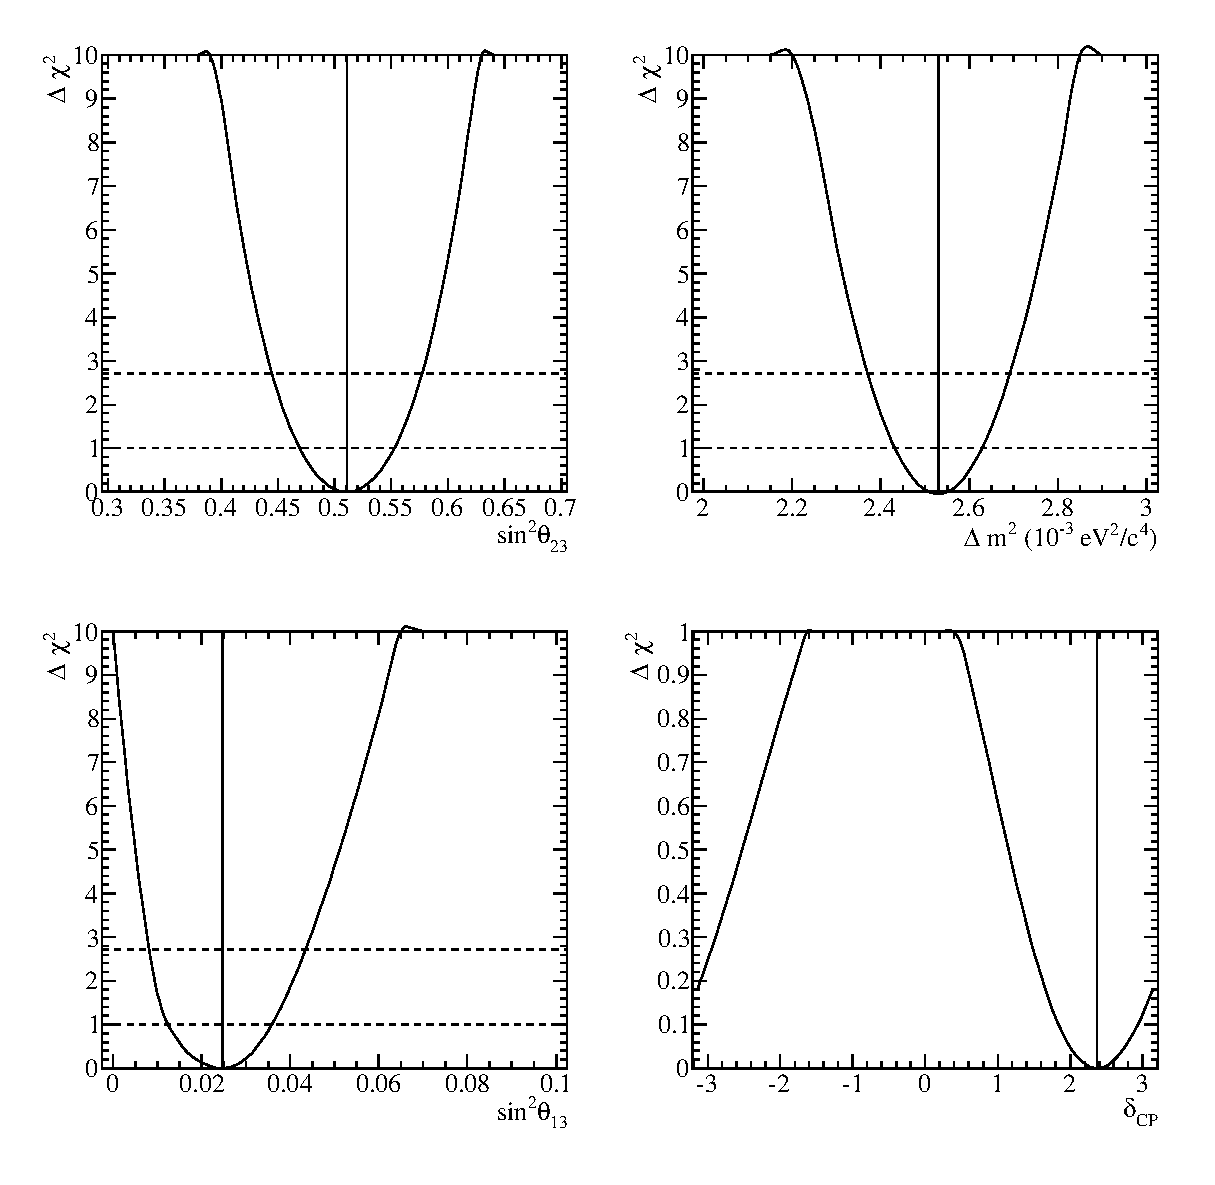
\includegraphics[width=25pc]{./images/validation/toy_dataset5_1D.eps}
\caption {
 $\Delta\chi^2$ as function of $\sin^{2}\theta_{23}$,$|\Delta m^{2}|$,$\sin^{2}\theta_{13}$ and $\delta_{CP}$
for fake dataset \#5 with inverted hierarchy (true one).
  At each point, $\chi^2$ was minimized with respect to the oscillation parameters not shown in each figure
and all 64 systematic parameters.
}
\label{fig:validation:toys:1D_toy5}
\end{center}

\vfill
\vspace*{0.7cm}

\begin{center}
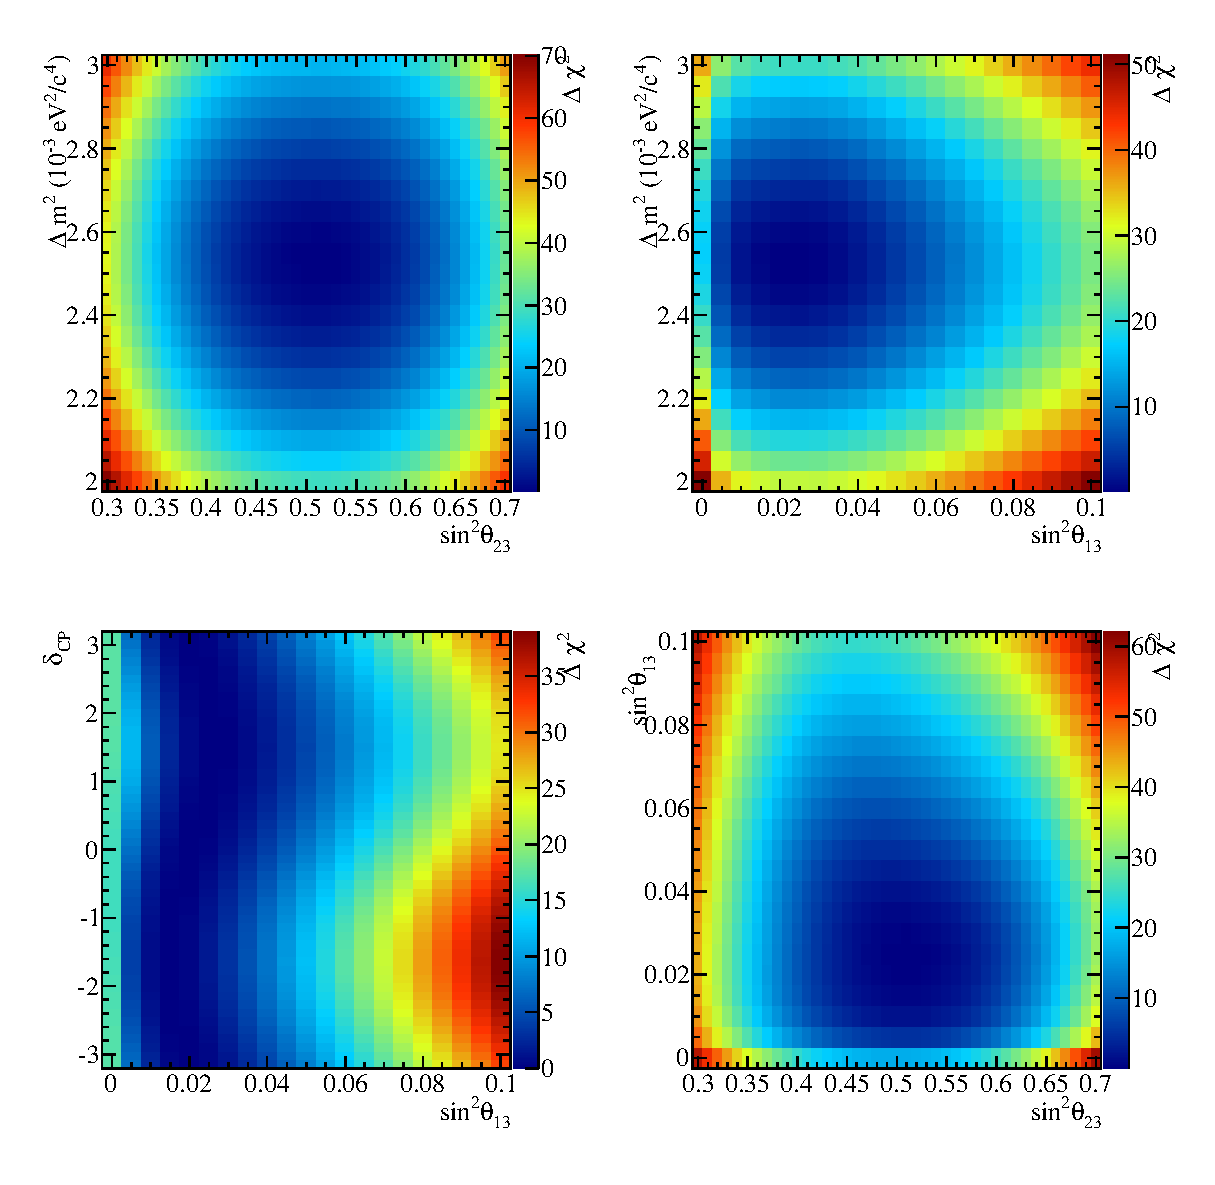
\includegraphics[width=30pc]{./images/validation/toy_dataset5_colz.eps}
\caption {
  $\Delta\chi^2$ surface in
($|\Delta m^{2}|$,$sin^{2}\theta_{23}$), 
($|\Delta m^{2}|$,$sin^{2}\theta_{13}$), 
($\delta_{CP}$,$sin^{2}\theta_{13}$) and 
($sin^{2}\theta_{13}$,$sin^{2}\theta_{23}$)
 spaces for fake dataset \#5 with inverted hierarchy (true one).
At each point, $\chi^2$ was minimized with respect to the oscillation parameters not shown in each figure
and all 64 systematic parameters.
}
\label{fig:validation:toys:colz_toy5}
\end{center}


\end{figure*}


\begin{figure*}[htb]
\begin{center}
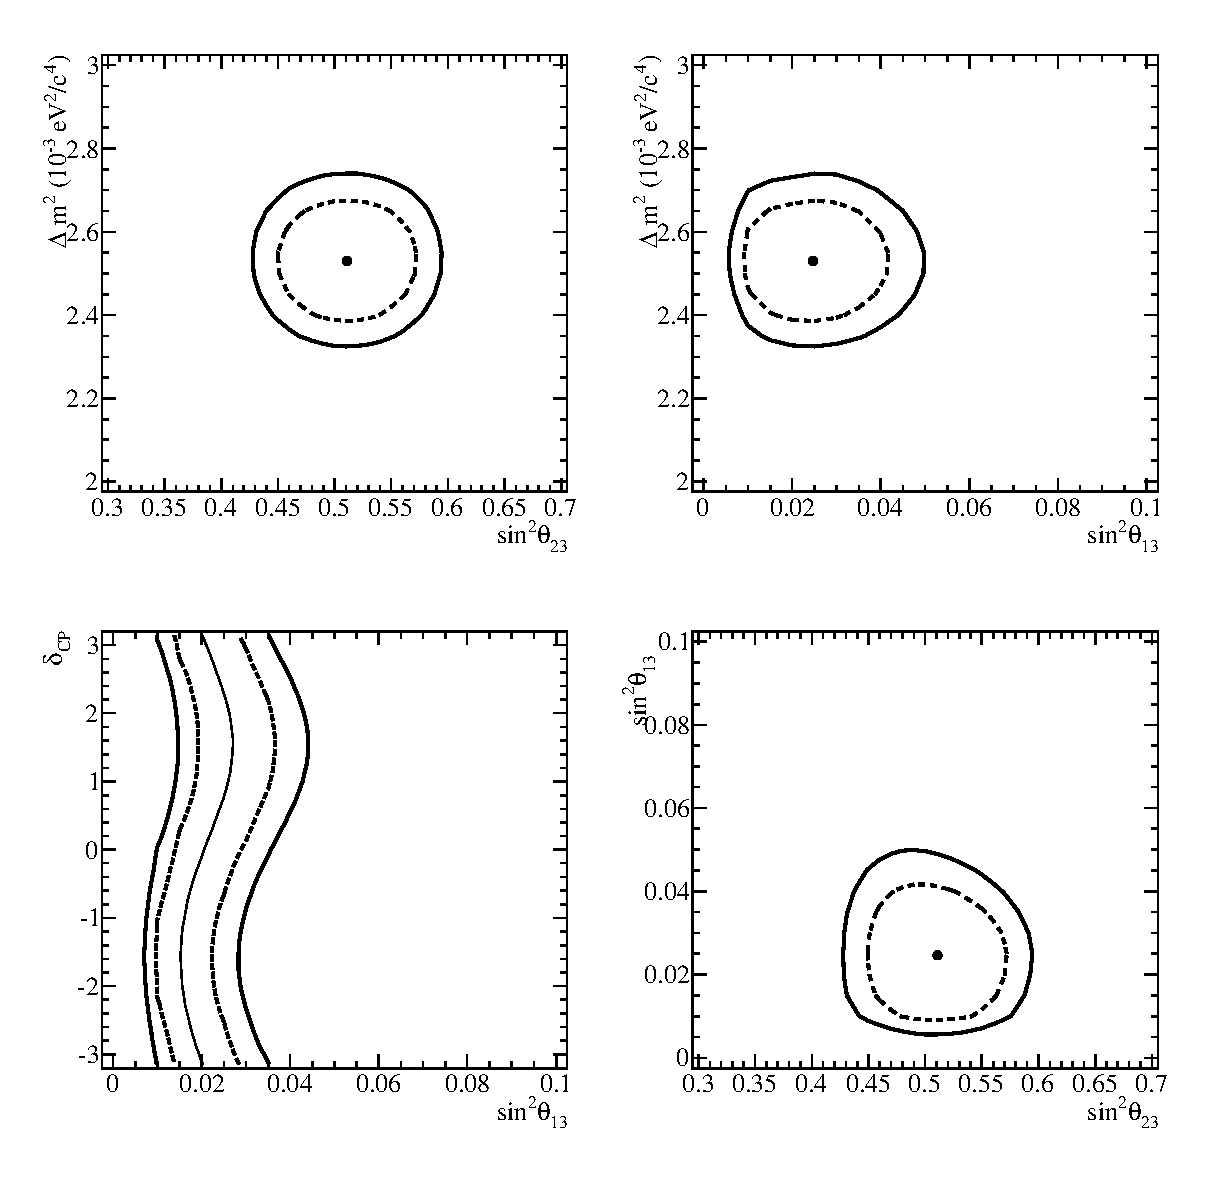
\includegraphics[width=40pc]{./images/validation/toy_dataset5_2D.eps}
\caption {
 68\% and 90\% CL regions in 
($|\Delta m^{2}|$,$sin^{2}\theta_{23}$), 
($|\Delta m^{2}|$,$sin^{2}\theta_{13}$), 
($\delta_{CP}$,$sin^{2}\theta_{13}$) and 
($sin^{2}\theta_{13}$,$sin^{2}\theta_{23}$)
 spaces for fake dataset \#5 with inverted hierarchy (true one).
At each point, $\chi^2$ was minimized with respect to the oscillation parameters not shown in each figure
and all 64 systematic parameters.
}
\label{fig:validation:toys:2D_toy5}
\end{center}
\end{figure*}


\begin{figure*}[htb]
\begin{center}
\begin{minipage}[t]{0.48\linewidth}

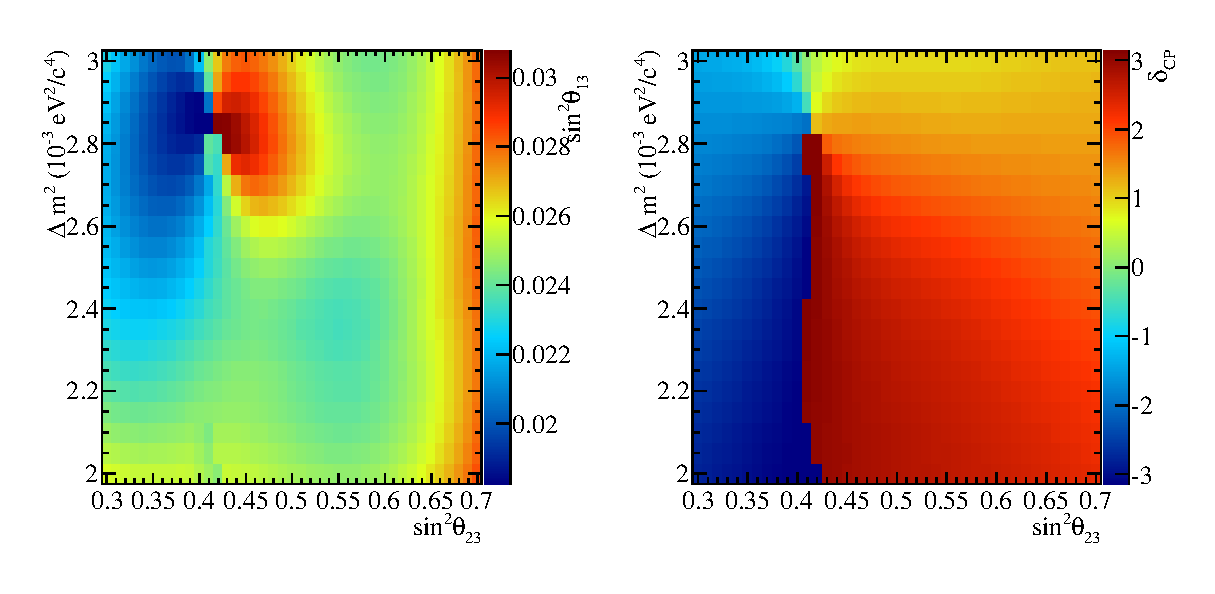
\includegraphics[width=10cm]{./images/validation/toy_dataset5_theta23_dmsq_extra.eps}
\caption {
 Best fit value of $sin^{2}\theta_{13}$ and $\delta_{CP}$
for the fit in the ($|\Delta m^{2}|$,$sin^{2}\theta_{23}$) space
for fake dataset \#5 with inverted hierarchy (true one).
}

\end{minipage}
\end{center}
\vfill
\vspace*{0.5cm}
\begin{center}
\begin{minipage}[t]{0.48\linewidth}

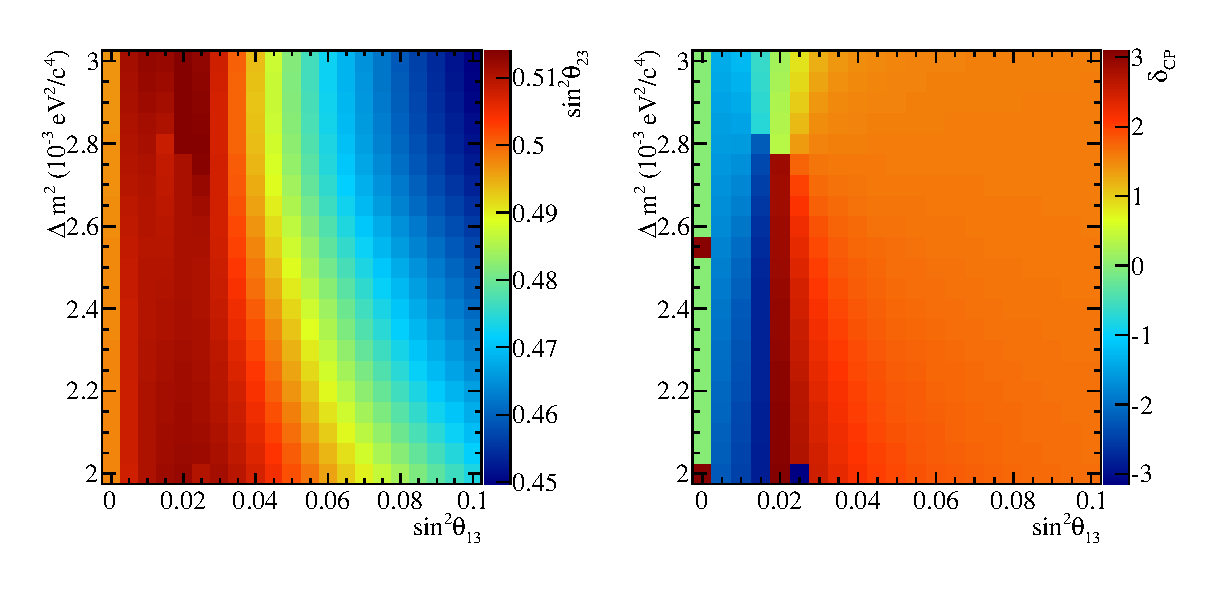
\includegraphics[width=10cm]{./images/validation/toy_dataset5_theta13_dmsq_extra.eps}
\caption {
 Best fit value of $sin^{2}\theta_{23}$ and $\delta_{CP}$
for the fit in the ($|\Delta m^{2}|$,$sin^{2}\theta_{13}$) space
for fake dataset \#5 with inverted hierarchy (true one).
}
\end{minipage}
\end{center}

\vfill
\vspace*{0.5cm}
\begin{center}
\begin{minipage}[t]{0.48\linewidth}

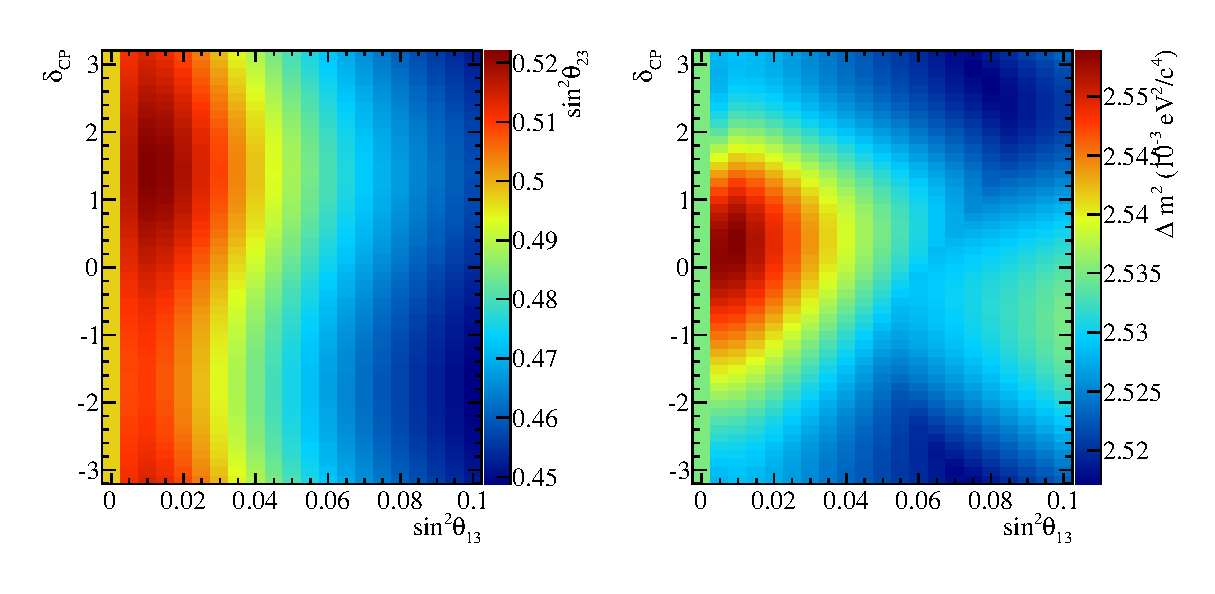
\includegraphics[width=10cm]{./images/validation/toy_dataset5_theta13_deltacp_extra.eps}
\caption {
 Best fit value of $sin^{2}\theta_{23}$ and $|\Delta m^{2}|$ 
for the fit in the ($\delta_{CP}$,$sin^{2}\theta_{23}$) space
for fake dataset \#5 with inverted hierarchy (true one).
}
\end{minipage}
\end{center}

\vfill
\vspace*{0.5cm}
\begin{center}
\begin{minipage}[t]{0.48\linewidth}

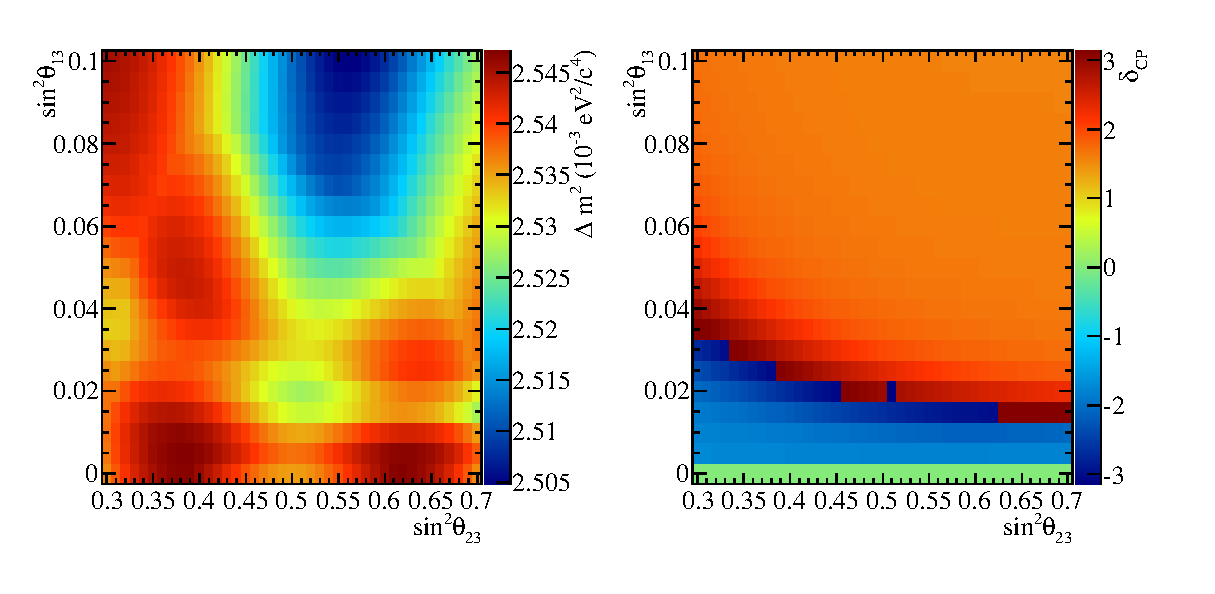
\includegraphics[width=10cm]{./images/validation/toy_dataset5_theta13_theta23_extra.eps}
\caption {
 Best fit value of $\delta_{CP}$ and $|\Delta m^{2}|$ 
for the fit in the ($sin^{2}\theta_{23}$,$sin^{2}\theta_{13}$) space
for fake dataset \#5 with inverted hierarchy (true one).
}
\end{minipage}
\end{center}

\label{fig:validation:toys:extra_toy5}
\end{figure*}


% 
% 
% ..............................................
% Fake dataset #5 with normal, comparison
% 
%
\clearpage

\begin{figure*}[htb]

\begin{center}
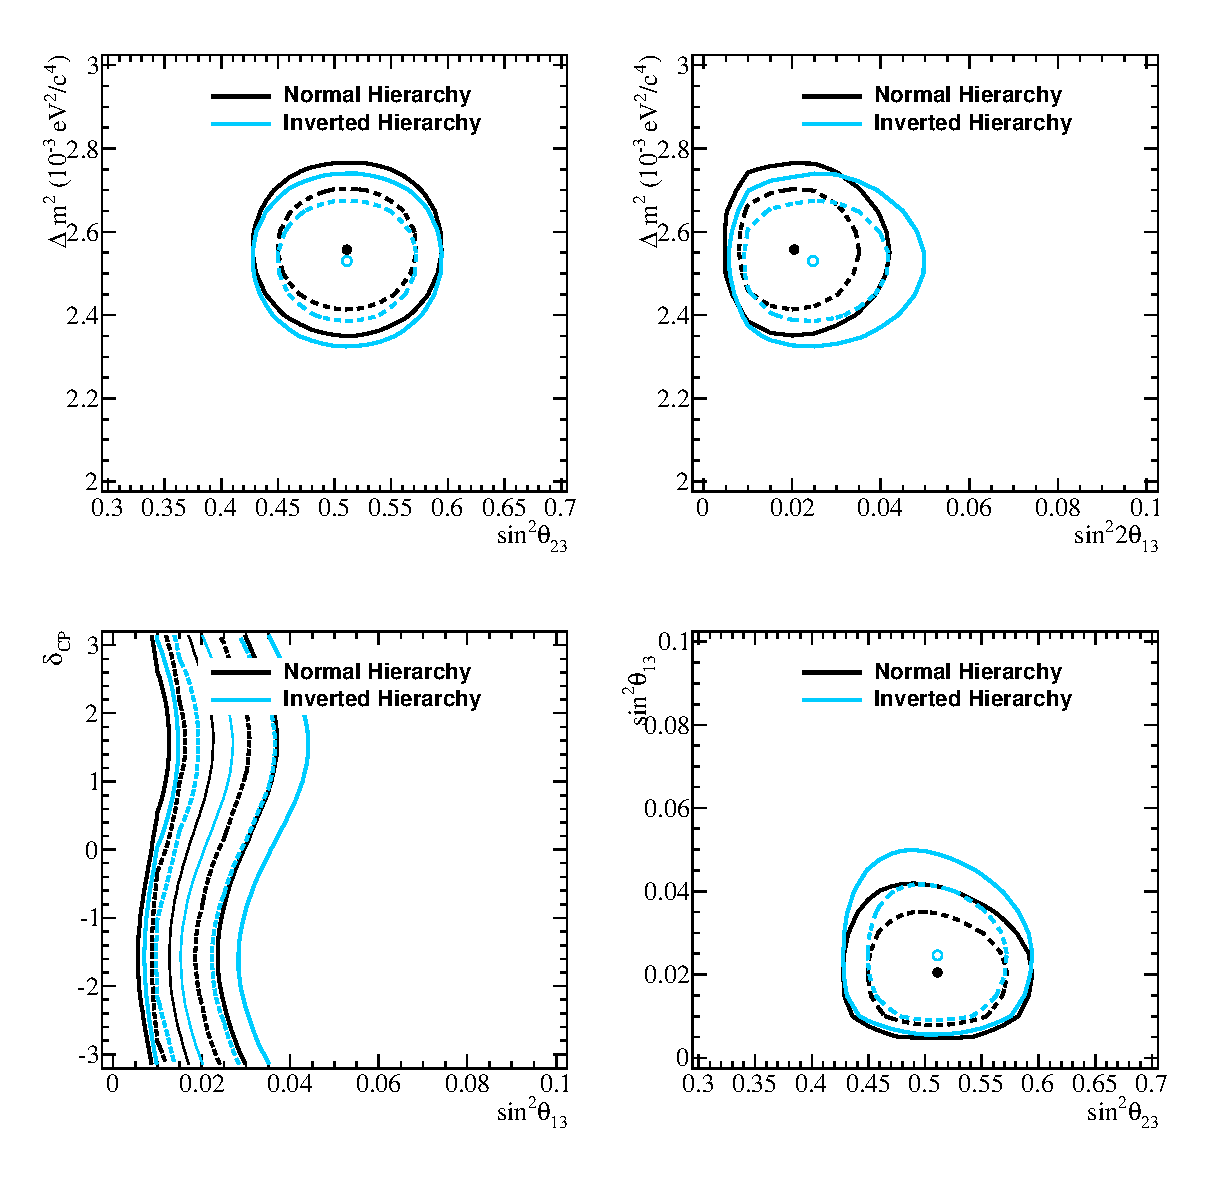
\includegraphics[width=40pc]{./images/validation/toy_dataset5_2D_comparison_mh.eps}
\caption {
 68\% and 90\% CL regions in 
($|\Delta m^{2}|$,$sin^{2}\theta_{23}$), 
($|\Delta m^{2}|$,$sin^{2}\theta_{13}$), 
($\delta_{CP}$,$sin^{2}\theta_{13}$) and 
($sin^{2}\theta_{13}$,$sin^{2}\theta_{23}$)
 spaces for fake dataset \#5 comparing results in inverted hierarchy (azure) and normal hierarchy (black).
At each point, $\chi^2$ was minimized with respect to the oscillation parameters not shown in each figure
and all 64 systematic parameters.
}
\label{fig:validation:toys:2D_toy5_comparison_mh}
\end{center}
\end{figure*}


%\begin{figure*}[htb]

%\begin{center}
%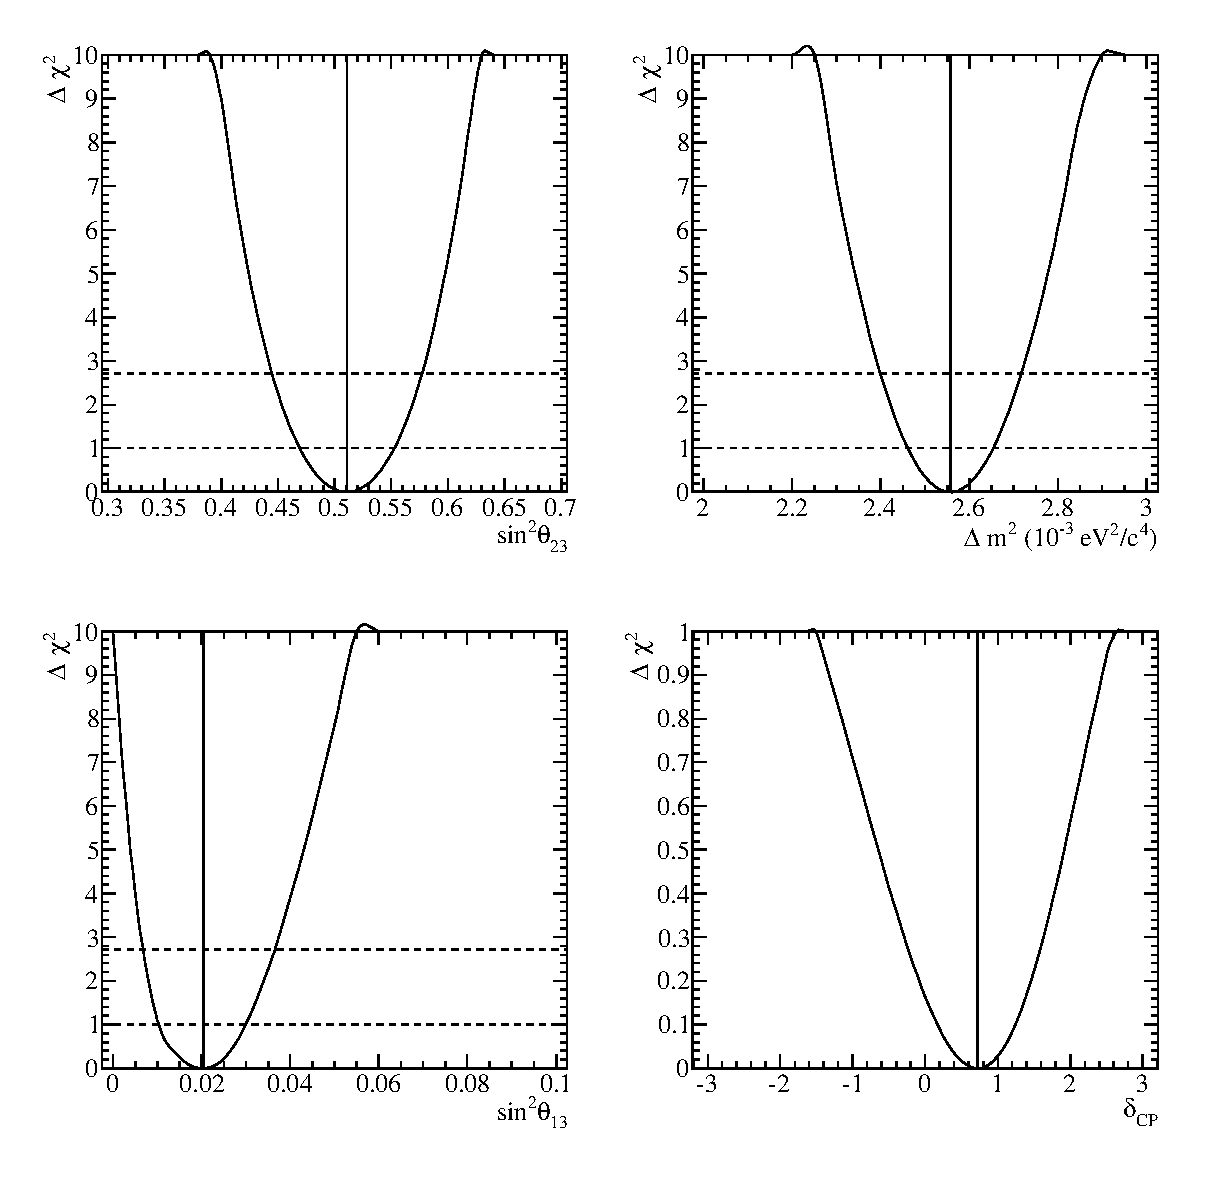
\includegraphics[width=25pc]{./images/validation/toy_dataset6_1D.eps}
%\caption {
 %$\Delta\chi^2$ as function of $\sin^{2}\theta_{23}$,$|\Delta m^{2}|$,$\sin^{2}\theta_{13}$ and $\delta_{CP}$
%for fake dataset \#5 with normal hierarchy.
 % At each point, $\chi^2$ was minimized with respect to the oscillation parameters not shown in each figure
%and all 64 systematic parameters.
%}
%\label{fig:validation:toys:1D_toy6}

%\vfill
%\vspace*{0.7cm}

%\begin{center}
%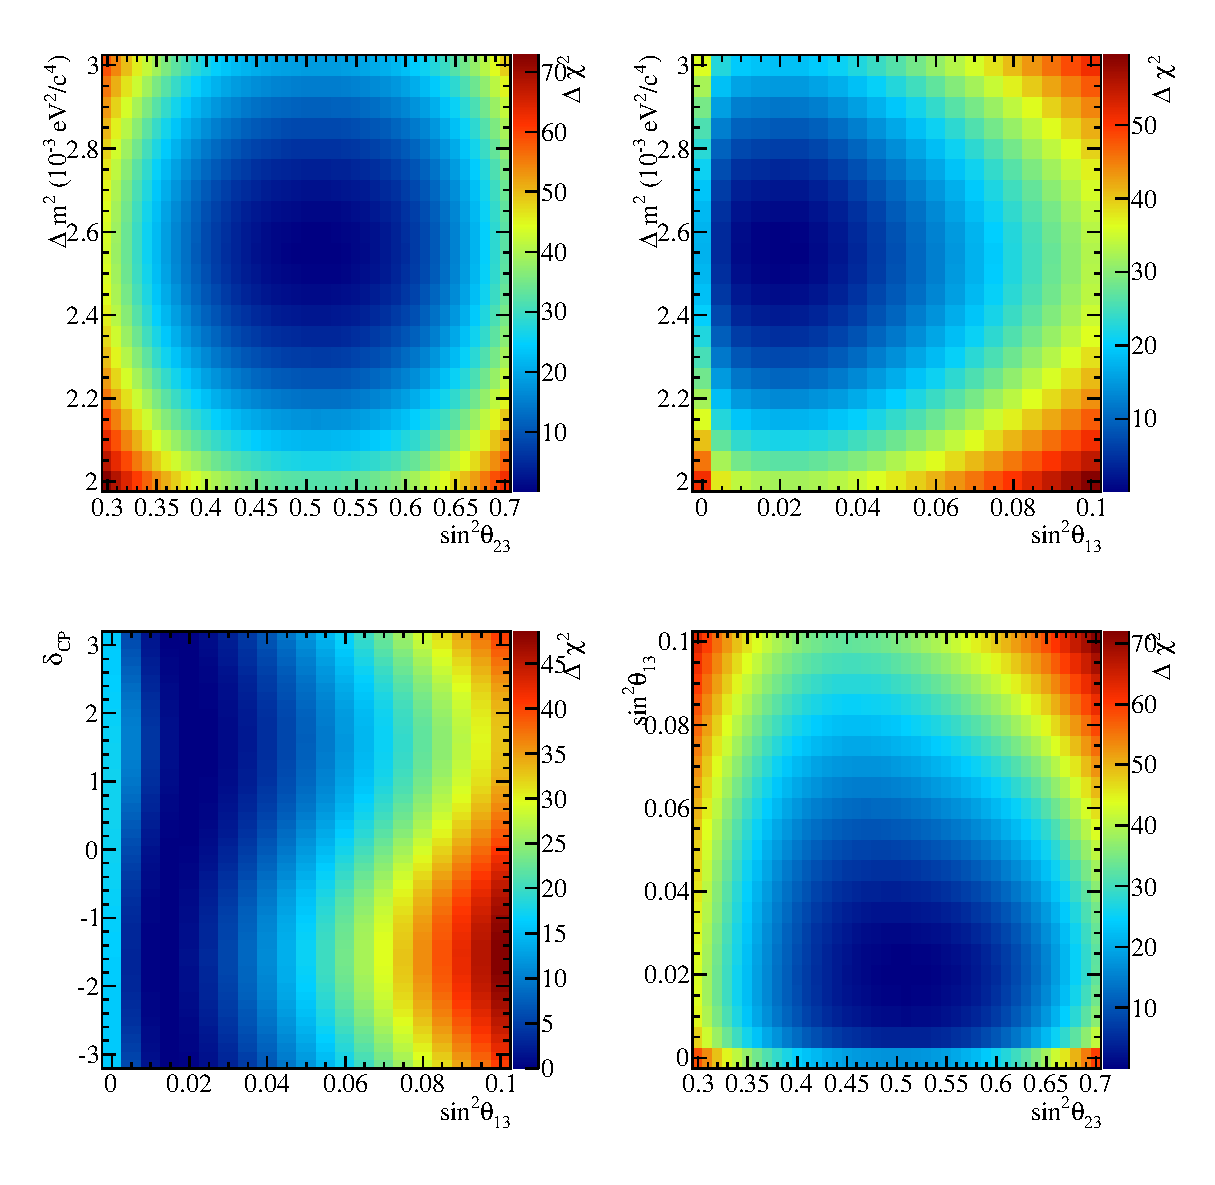
\includegraphics[width=30pc]{./images/validation/toy_dataset6_colz.eps}
%\caption {
 % $\Delta\chi^2$ surface in
%($|\Delta m^{2}|$,$sin^{2}\theta_{23}$), 
%($|\Delta m^{2}|$,$sin^{2}\theta_{13}$), 
%($\delta_{CP}$,$sin^{2}\theta_{13}$) and 
%($sin^{2}\theta_{13}$,$sin^{2}\theta_{23}$)
 %spaces for fake dataset \#5 with normal hierarchy.
%At each point, $\chi^2$ was minimized with respect to the oscillation parameters not shown in each figure
%and all 64 systematic parameters.
%}
%\label{fig:validation:toys:colz_toy6}


%\end{figure*}


%\begin{figure*}[htb]



%\begin{center}
%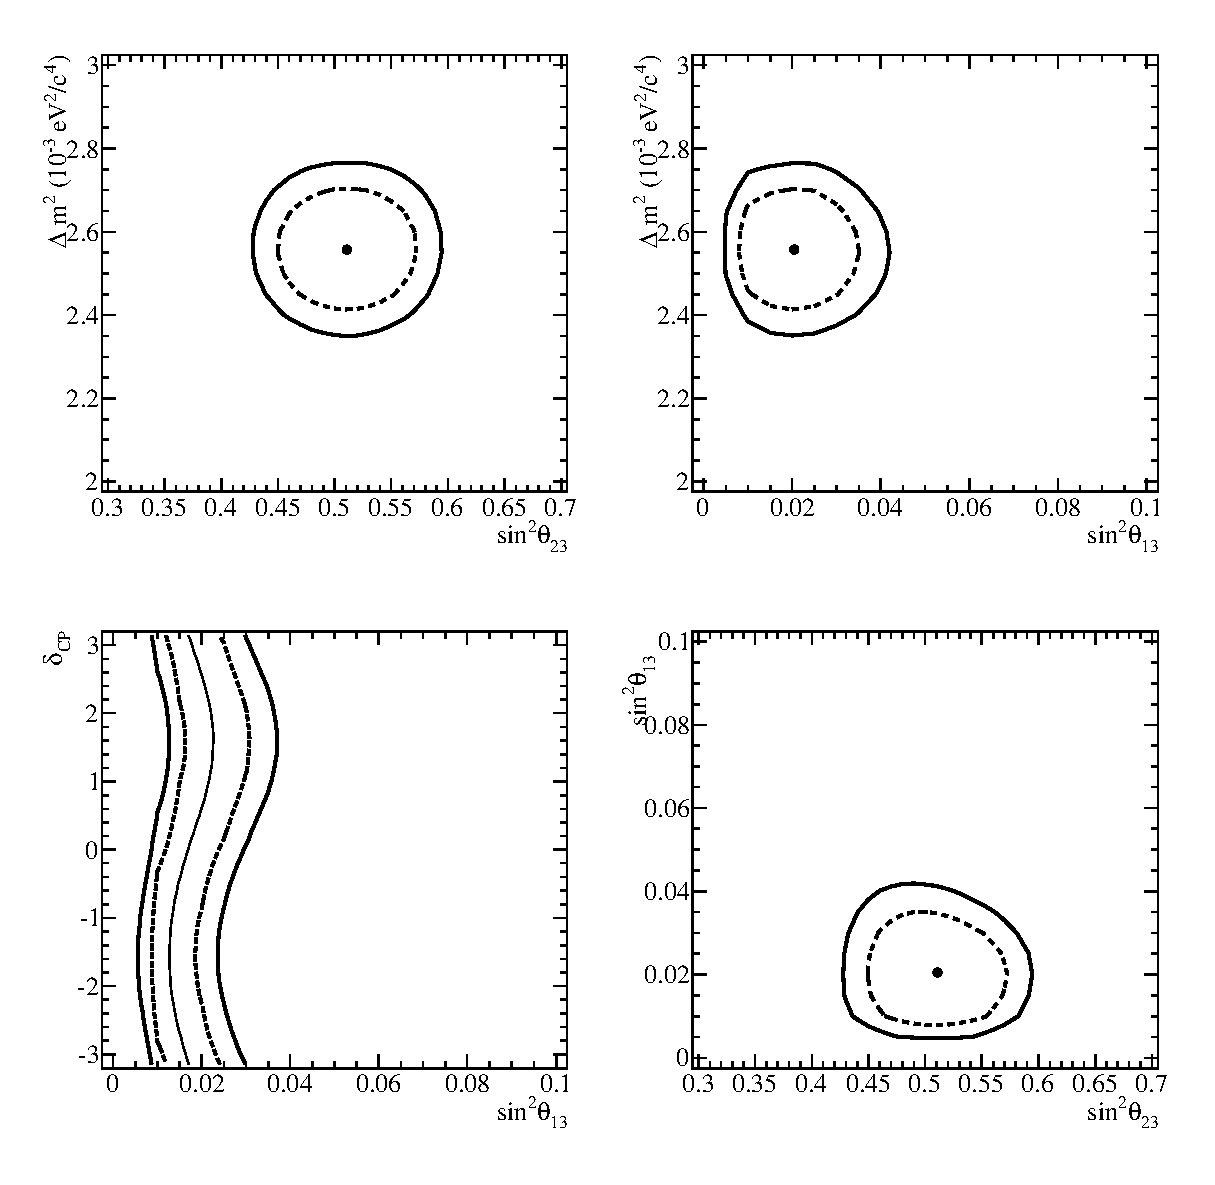
\includegraphics[width=40pc]{./images/validation/toy_dataset6_2D.eps}
%\caption {
 %68\% and 90\% CL regions in 
%($|\Delta m^{2}|$,$sin^{2}\theta_{23}$), 
%($|\Delta m^{2}|$,$sin^{2}\theta_{13}$), 
%($\delta_{CP}$,$sin^{2}\theta_{13}$) and 
%($sin^{2}\theta_{13}$,$sin^{2}\theta_{23}$)
% spaces for fake dataset \#5 with normal hierarchy.
%At each point, $\chi^2$ was minimized with respect to the oscillation parameters not shown in each figure
%and all 64 systematic parameters.
%}
%\label{fig:validation:toys:2D_toy6}
%\end{figure*}


%\begin{figure*}[htb]
%\begin{center}
%\begin{minipage}[t]{0.48\linewidth}

%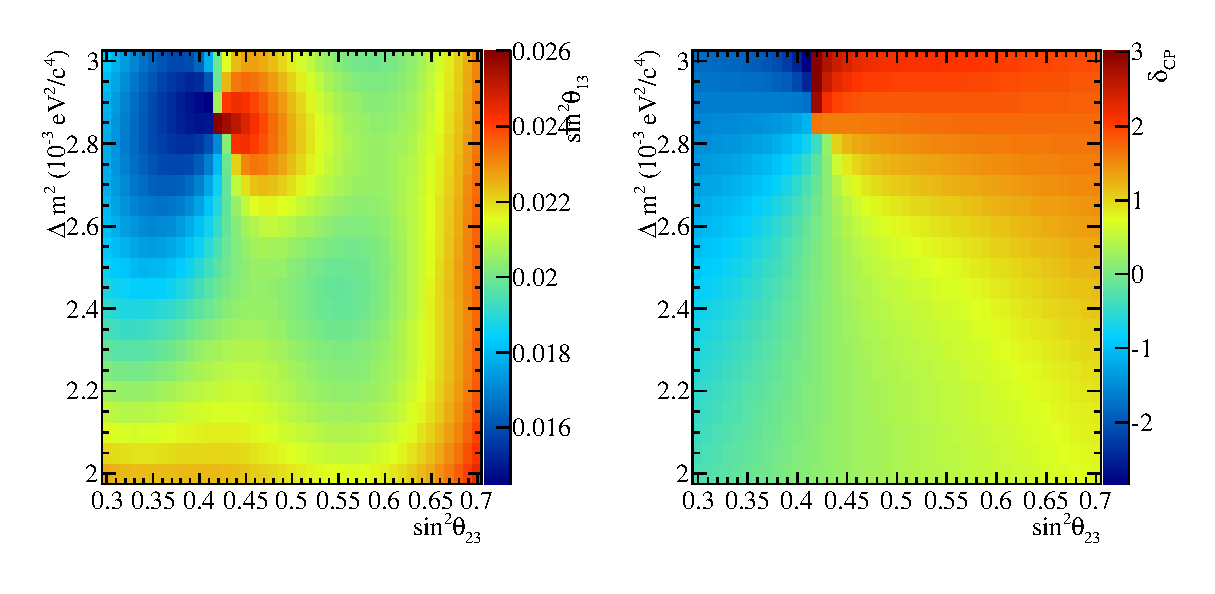
\includegraphics[width=10cm]{./images/validation/toy_dataset6_theta23_dmsq_extra.eps}
%\caption {
 %Best fit value of $sin^{2}\theta_{13}$ and $\delta_{CP}$
%for the fit in the ($|\Delta m^{2}|$,$sin^{2}\theta_{23}$) space
%for fake dataset \#5 with normal hierarchy.
%}

%\end{minipage}
%\vfill
%\vspace*{0.5cm}
%\begin{center}
%\begin{minipage}[t]{0.48\linewidth}

%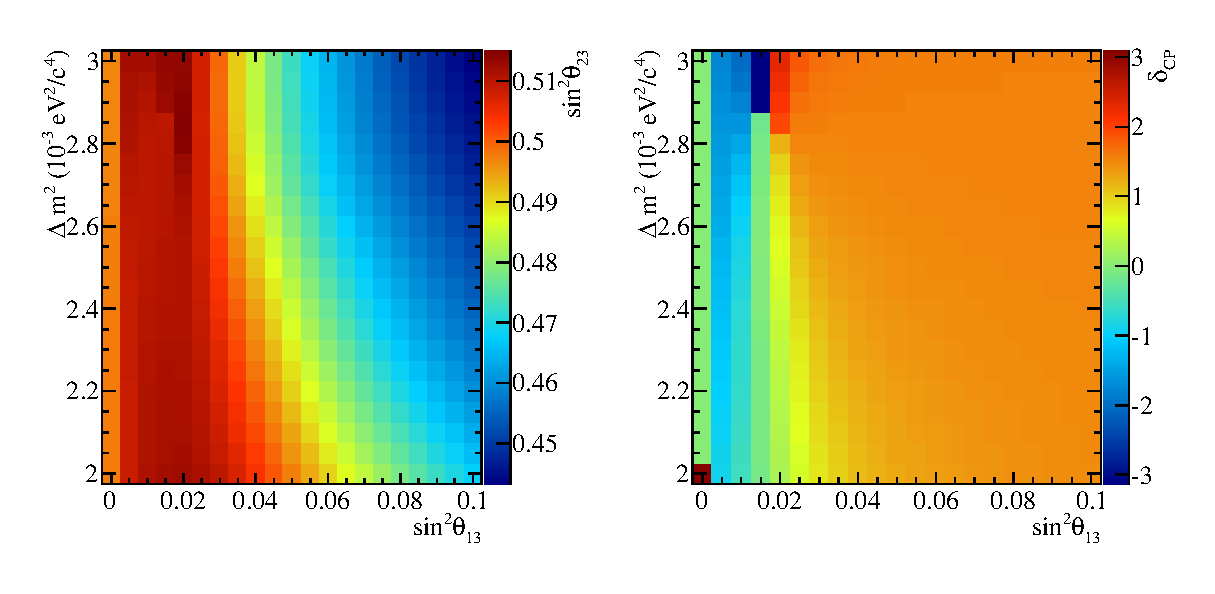
\includegraphics[width=10cm]{./images/validation/toy_dataset6_theta13_dmsq_extra.eps}
%\caption {
 %Best fit value of $sin^{2}\theta_{23}$ and $\delta_{CP}$
%for the fit in the ($|\Delta m^{2}|$,$sin^{2}\theta_{13}$) space
%for fake dataset \#5 with normal hierarchy.
%}

%\end{minipage}
%\vfill
%\vspace*{0.5cm}
%\begin{center}
%\begin{minipage}[t]{0.48\linewidth}

%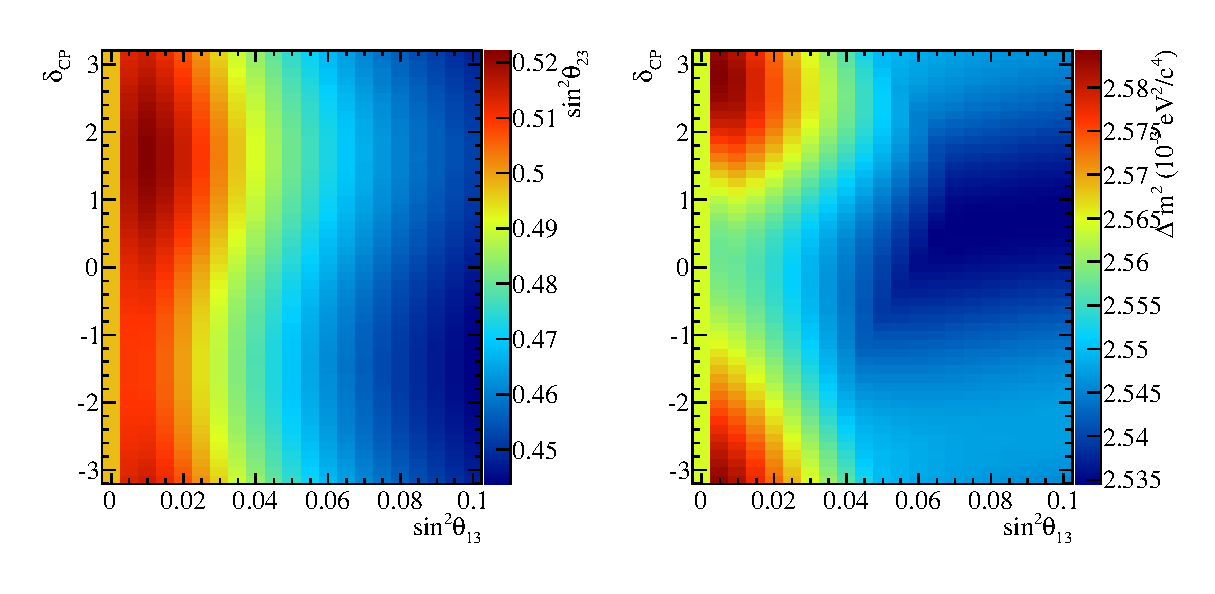
\includegraphics[width=10cm]{./images/validation/toy_dataset6_theta13_deltacp_extra.eps}
%\caption {
 %Best fit value of $sin^{2}\theta_{23}$ and $|\Delta m^{2}|$ 
%for the fit in the ($\delta_{CP}$,$sin^{2}\theta_{23}$) space
%for fake dataset \#5 with normal hierarchy.
%}

%\end{minipage}
%\vfill
%\vspace*{0.5cm}
%\begin{center}
%\begin{minipage}[t]{0.48\linewidth}

%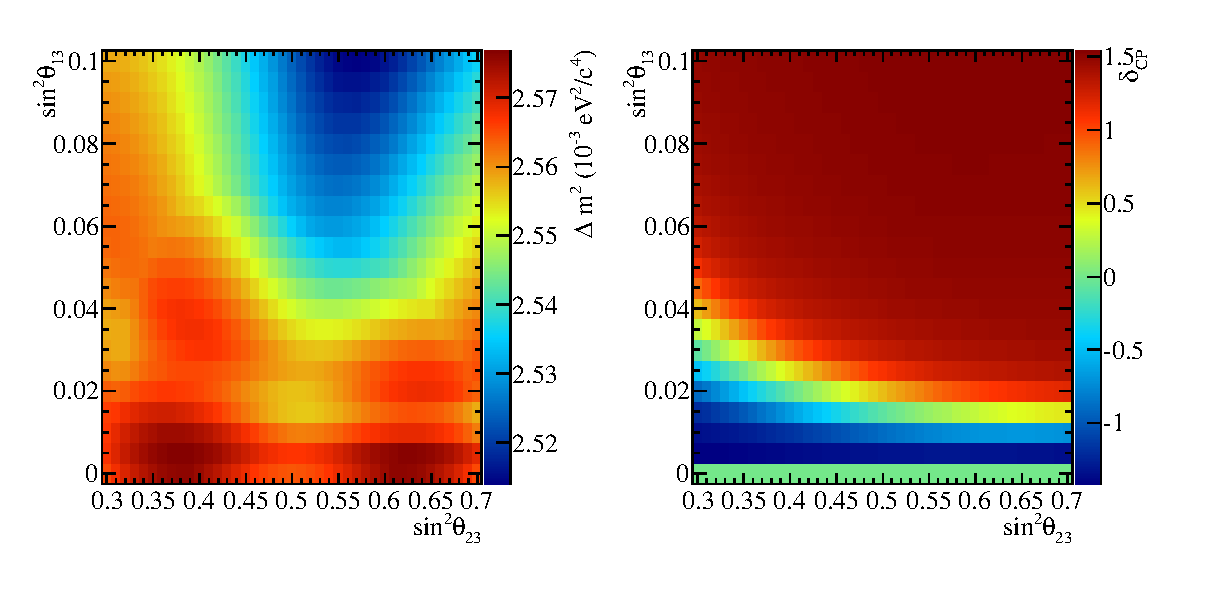
\includegraphics[width=10cm]{./images/validation/toy_dataset6_theta13_theta23_extra.eps}
%\caption {
 %Best fit value of $\delta_{CP}$ and $|\Delta m^{2}|$ 
%for the fit in the ($sin^{2}\theta_{23}$,$sin^{2}\theta_{13}$) space
%for fake dataset \#5 with normal hierarchy.
%}

%\end{minipage}

%\label{fig:validation:toys:extra_toy6}
%\end{figure*}



% 
% 
% ..............................................
% Fake dataset #1 comparison using sinsqtheta13 and sinsq2theta13
% 
%
\clearpage
\begin{figure}[htbp]
\begin{center}
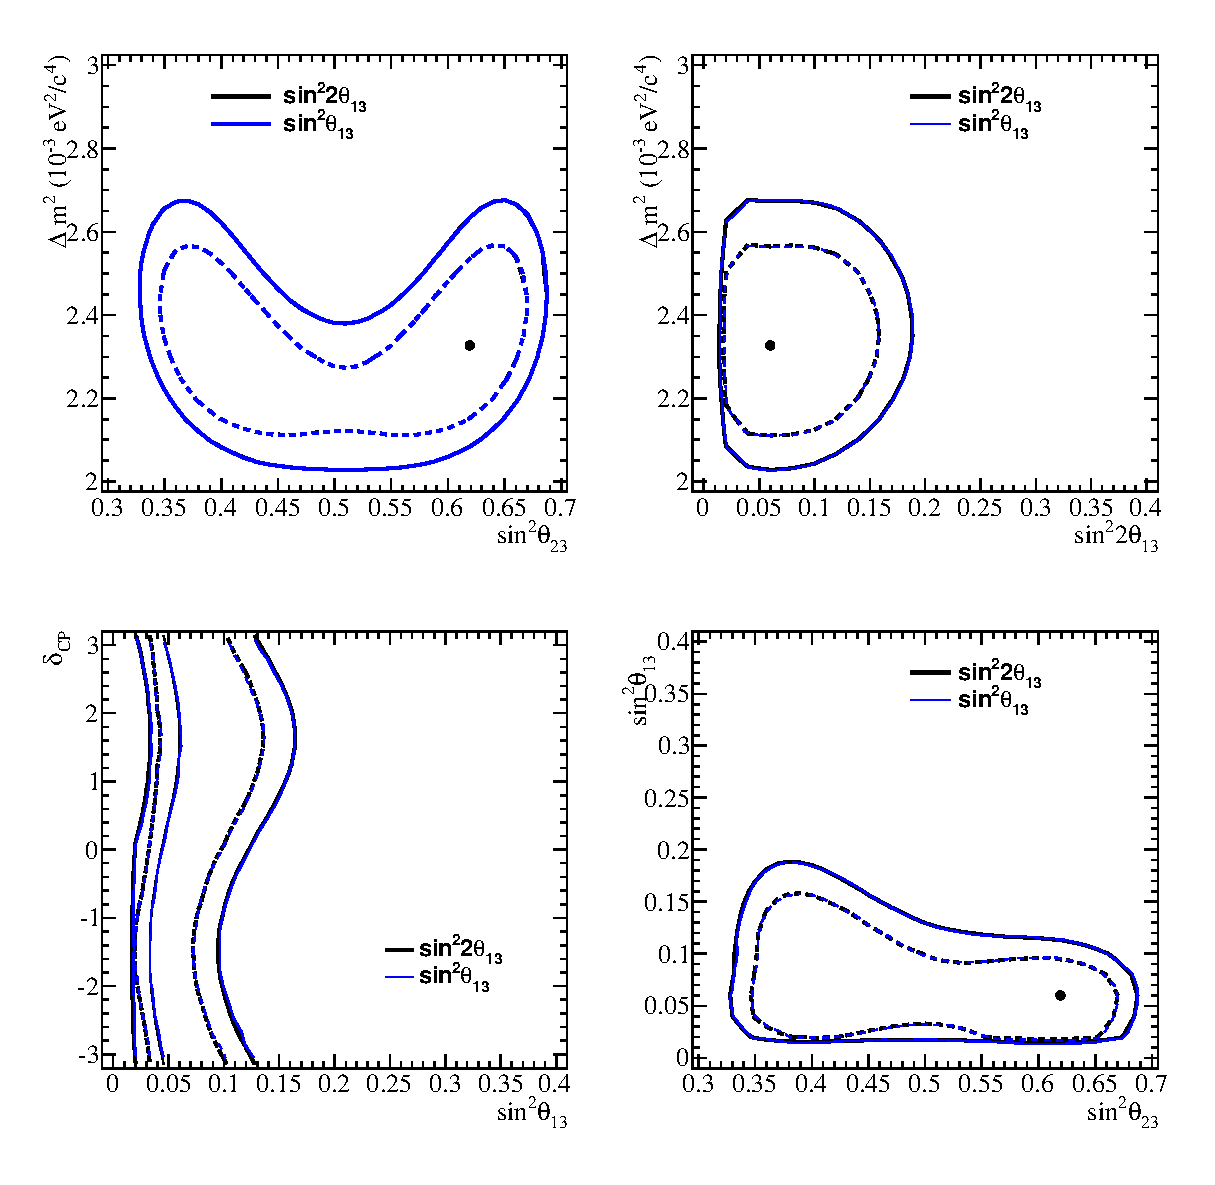
\includegraphics[width=40pc]{./images/validation/toy_dataset1_2D_comparison.eps}
\caption {
68\% and 90\% CL regions in 
($|\Delta m^{2}|$,$sin^{2}\theta_{23}$), 
($|\Delta m^{2}|$,$sin^{2}\theta_{13}$), 
($\delta_{CP}$,$sin^{2}\theta_{13}$) and 
($sin^{2}\theta_{13}$,$sin^{2}\theta_{23}$)
 spaces for fake dataset \#1 comparing results using $sin^{2}\theta_{13}$ (blue) and $sin^{2}2\theta_{13}$ (black).
At each point, $\chi^2$ was minimized with respect to the oscillation parameters not shown in each figure
and all 64 systematic parameters.
}
\label{fig:validation:toys:2D_toy1_comparison}
\end{center}
\end{figure}


\begin{figure}[htbp]
\begin{center}
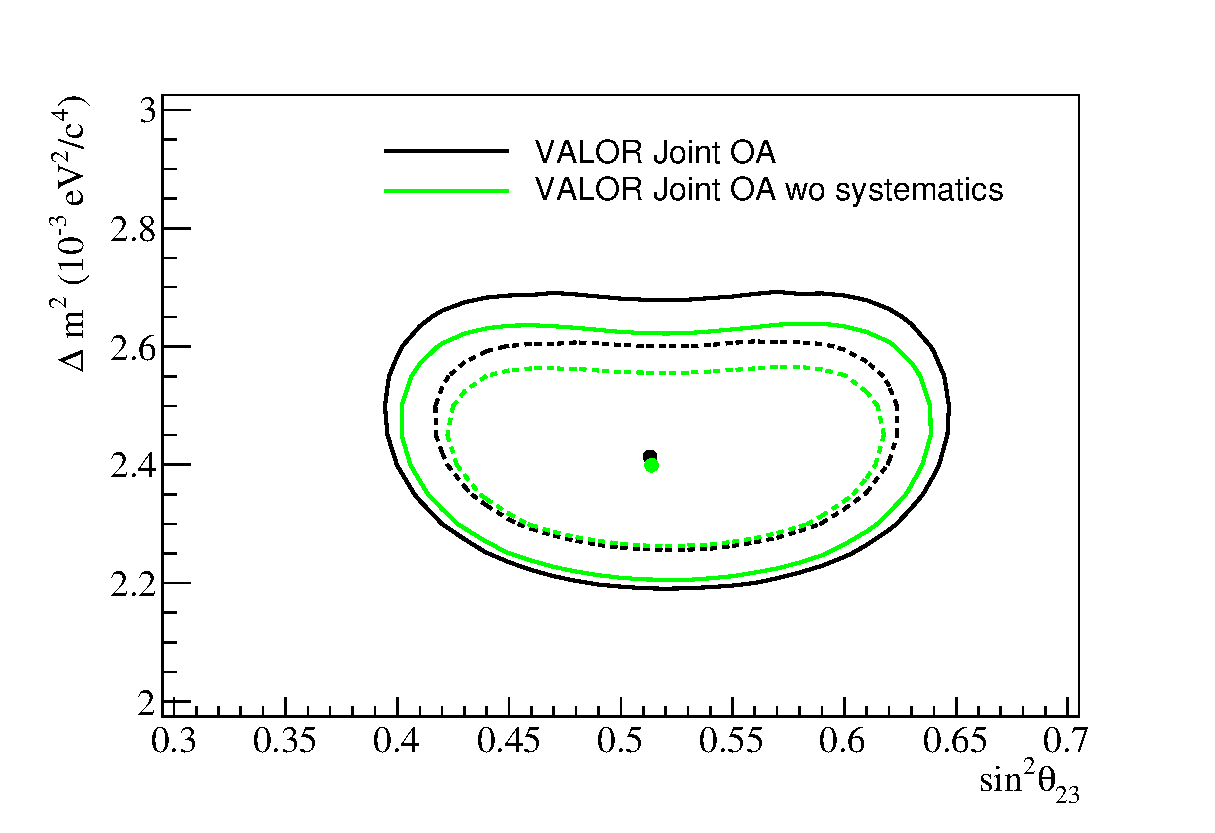
\includegraphics[width=20pc]{./images/validation/Comparison_with_wo_syst_toy0.eps}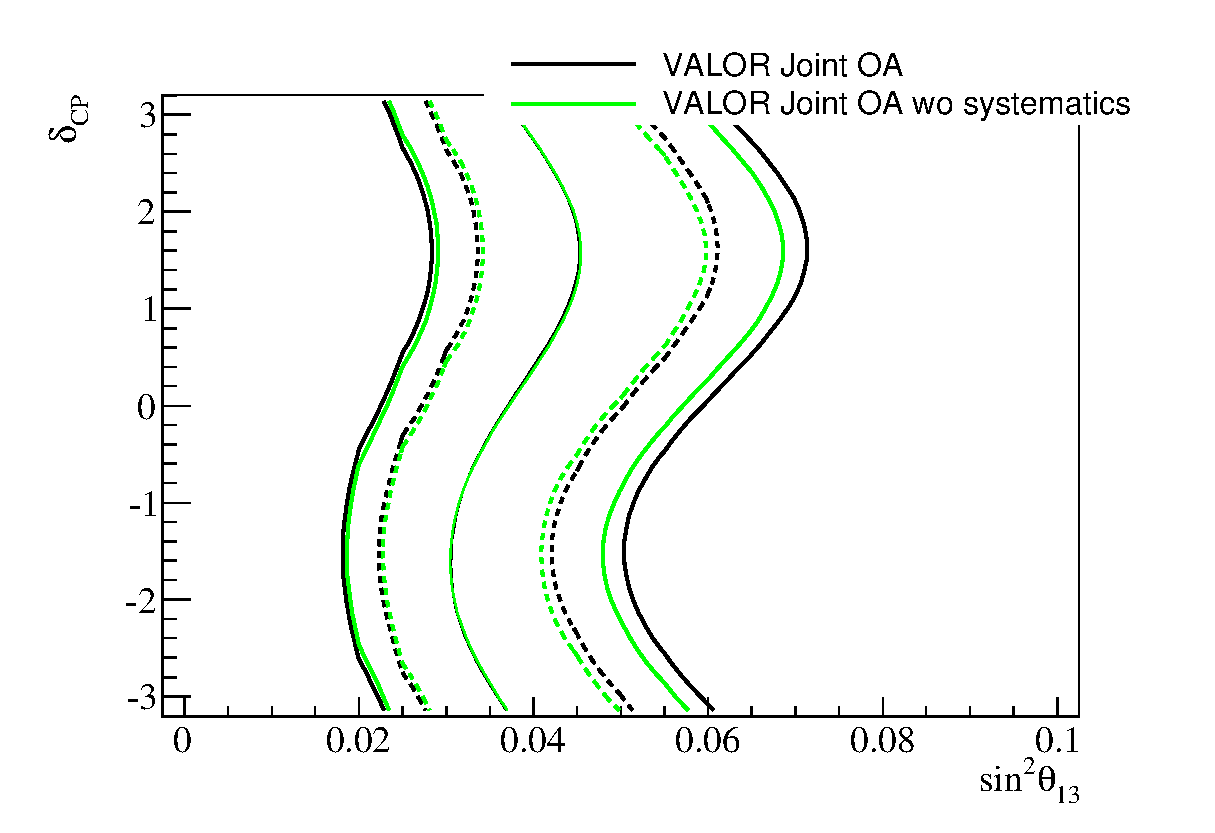
\includegraphics[width=20pc]{./images/validation/Comparison_with_wo_syst_toy0_theta13_deltacp.eps}
\caption {
68\% and 90\% CL regions in 
($|\Delta m^{2}|$,$sin^{2}\theta_{23}$) and
($\delta_{CP}$,$sin^{2}\theta_{13}$)
 spaces for fake dataset \#0 comparing results with (black) and without (green) including systematic parameters in the fit.
}
\label{fig:validation:toys:toy0wosyst}
\end{center}
\end{figure}


\clearpage
\begin{figure}[htb]
\begin{minipage}[t]{0.48\linewidth}
\center
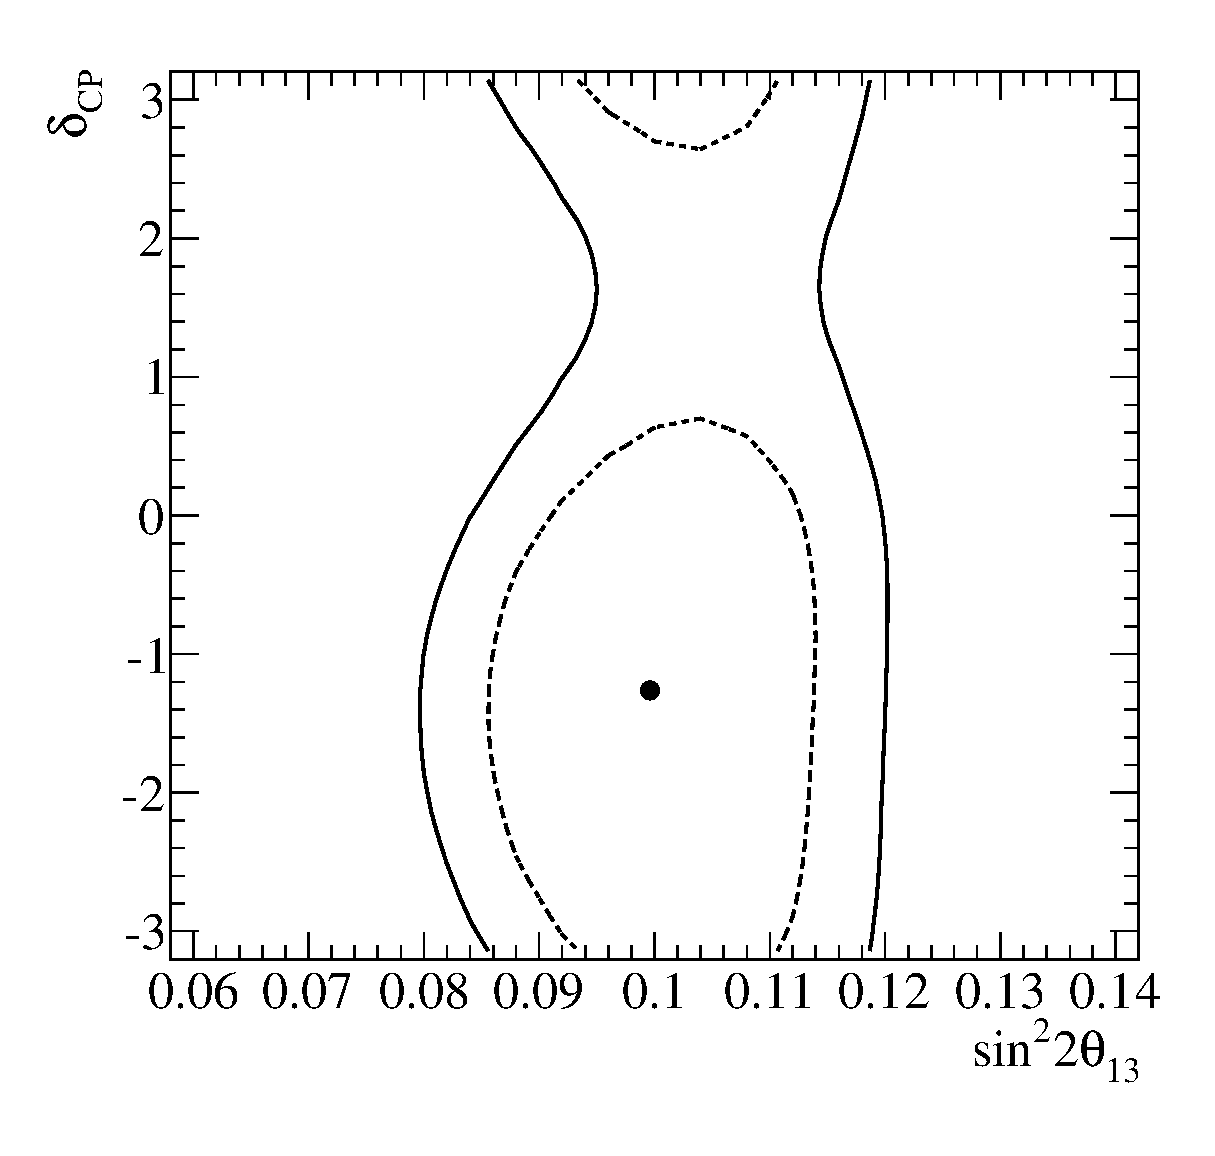
\includegraphics[width=7cm]{./images/validation/toy_dataset0_fit_joint_nh_reactor_2D.eps}
\caption {
 Confidence regions in the ($sin^{2}2\theta_{13}$,$\delta_{CP}$)
parameter space for fake dataset \#0 including constraint in $sin^{2}2\theta_{13}$,
assuming normal hierarchy.
}
\label{fig:validation:toys:reactor_toy0}
\end{minipage}
\hspace{0.02\linewidth}
\begin{minipage}[t]{0.48\linewidth}
\center
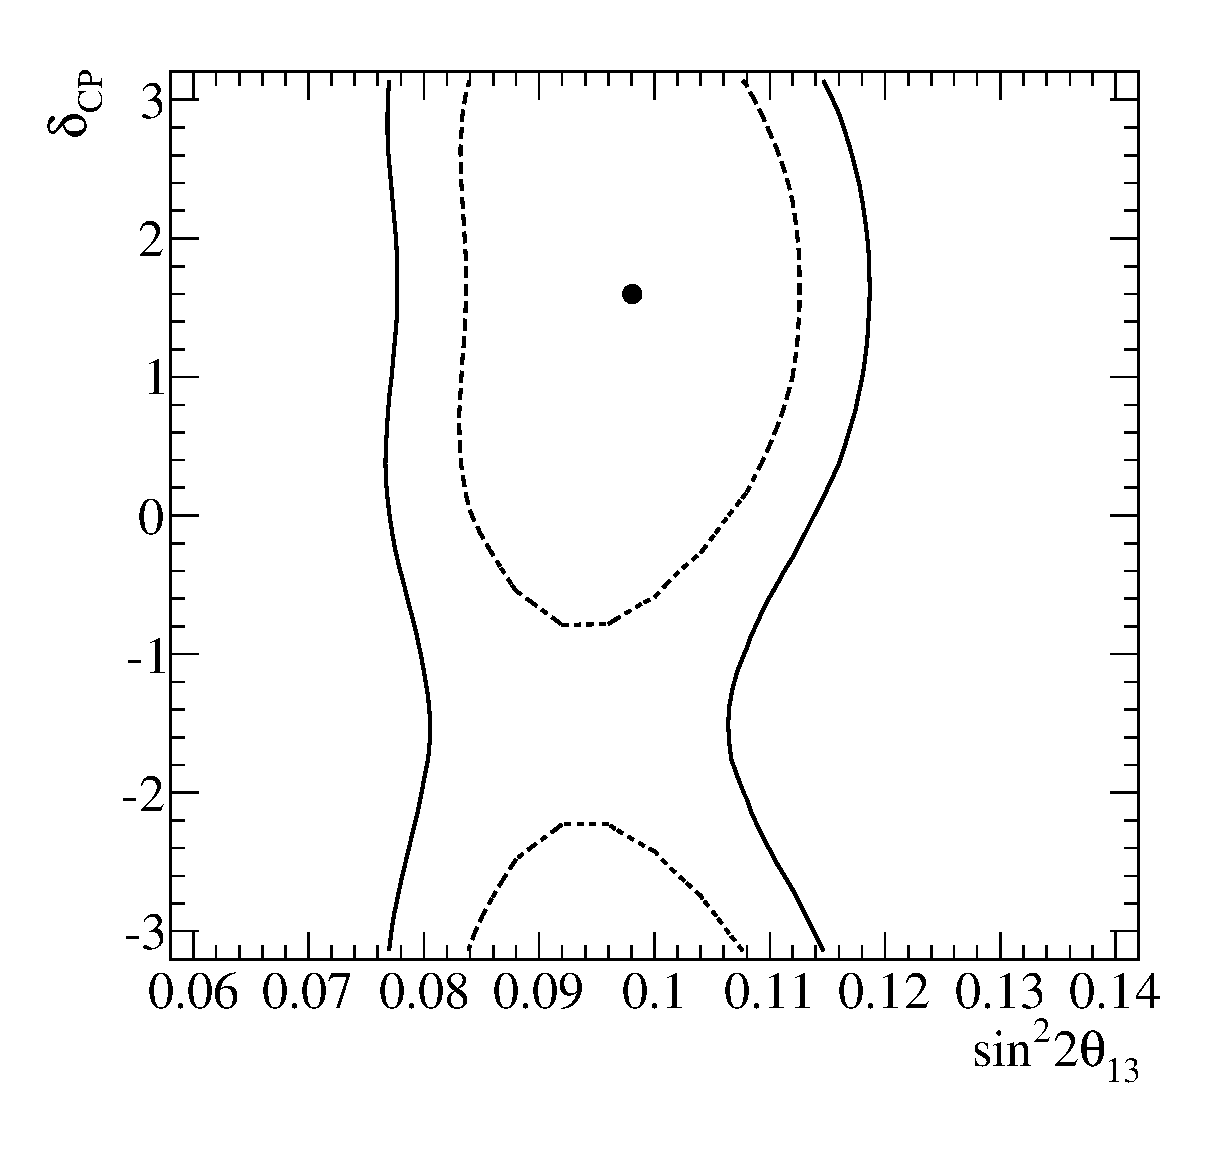
\includegraphics[width=7cm]{./images/validation/toy_dataset1_fit_joint_nh_reactor_2D.eps}
\caption {
 Confidence regions in the ($sin^{2}2\theta_{13}$,$\delta_{CP}$)
parameter space for fake dataset \#1 including constraint in $sin^{2}2\theta_{13}$,
assuming normal hierarchy.
}
\label{fig:validation:toys:reactor_toy1}
\end{minipage}
\vfill
\vspace*{0.5cm}
\begin{minipage}[t]{0.48\linewidth}
\center
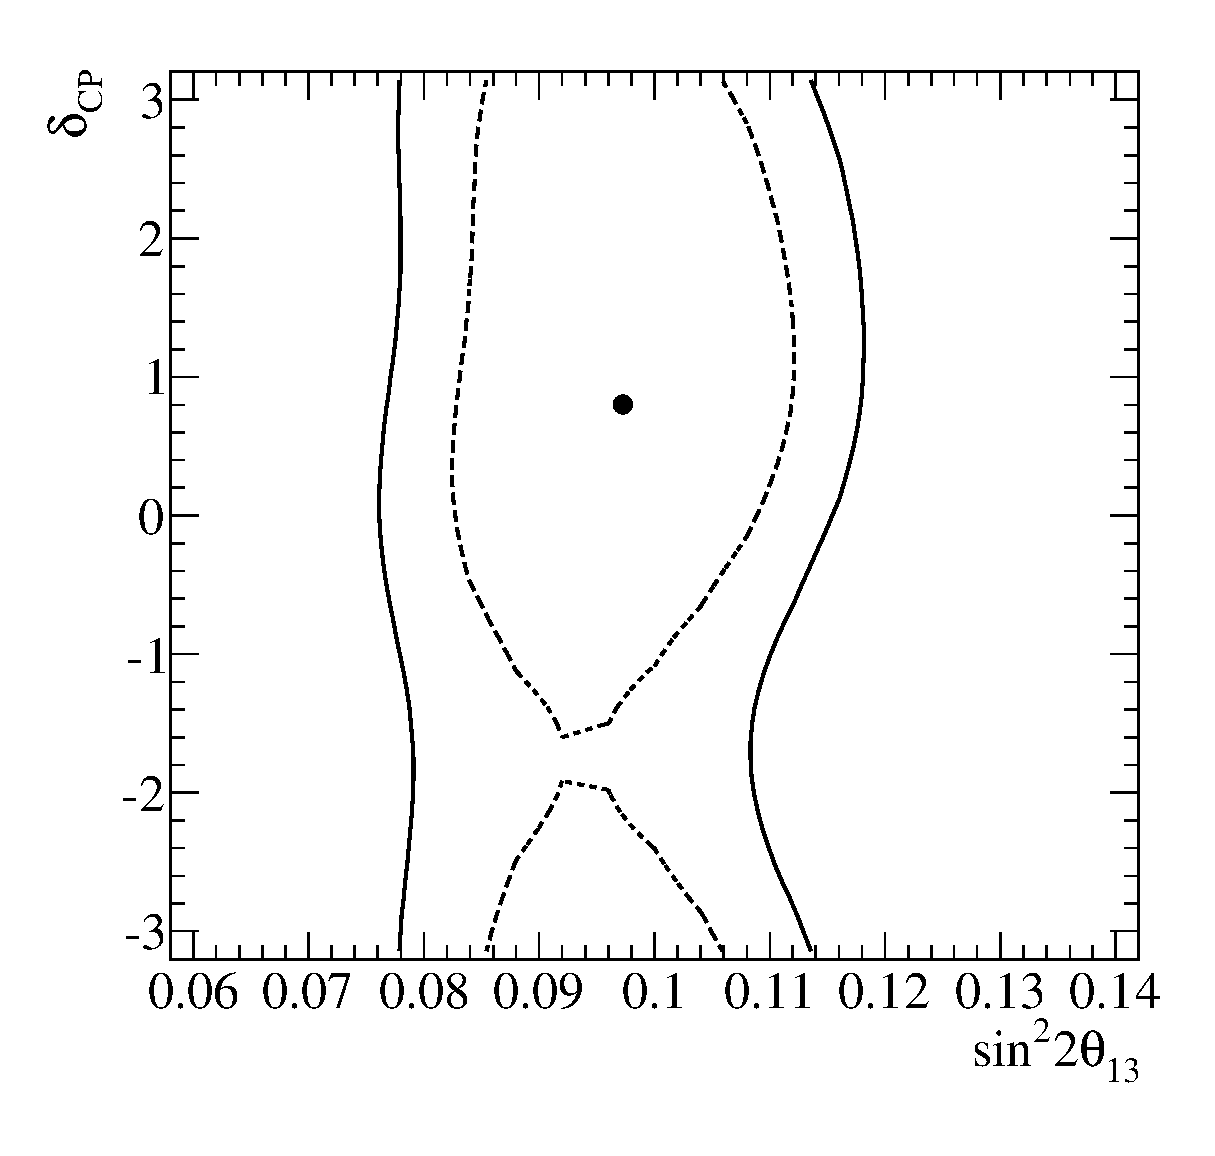
\includegraphics[width=7cm]{./images/validation/toy_dataset2_fit_joint_nh_reactor_2D.eps}
\caption {
 Confidence regions in the ($sin^{2}2\theta_{13}$,$\delta_{CP}$)
parameter space for fake dataset \#2 including constraint in $sin^{2}2\theta_{13}$,
assuming normal hierarchy.
}
\label{fig:validation:toys:reactor_toy2}
\end{minipage}
\hspace{0.02\linewidth}
\begin{minipage}[t]{0.48\linewidth}
\center
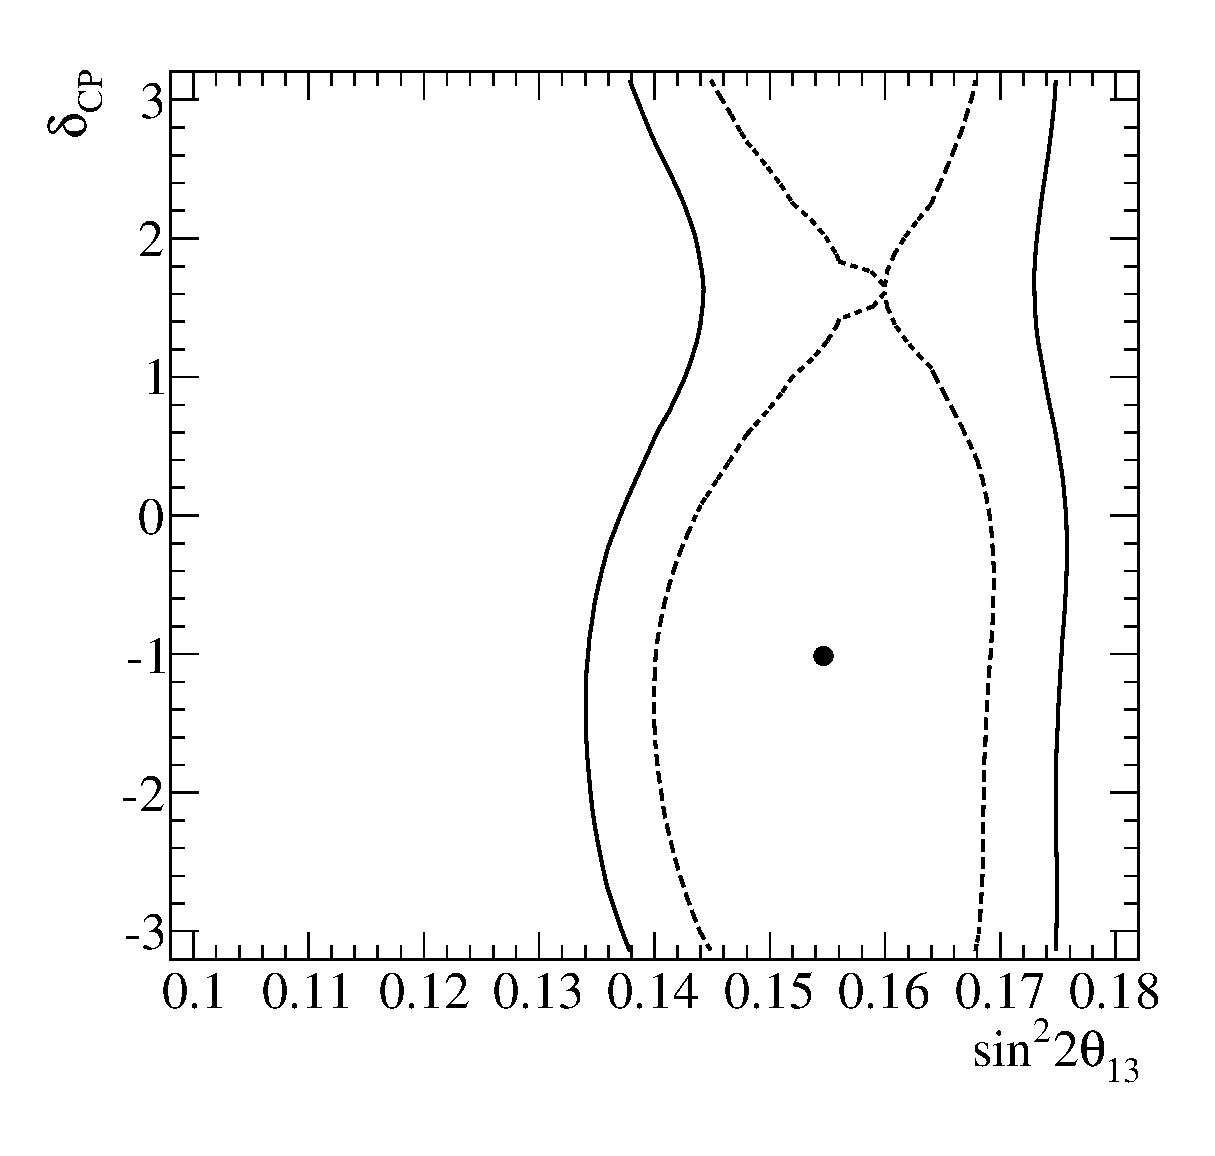
\includegraphics[width=7cm]{./images/validation/toy_dataset3_fit_joint_nh_reactor_2D.eps}
\caption {
 Confidence regions in the ($sin^{2}2\theta_{13}$,$\delta_{CP}$)
parameter space for fake dataset \#3 including constraint in $sin^{2}2\theta_{13}$,
assuming normal hierarchy.
}
\label{fig:validation:toys:reactor_toy3}
\end{minipage}
\vfill
\vspace*{0.5cm}
\begin{minipage}[t]{0.48\linewidth}
\center
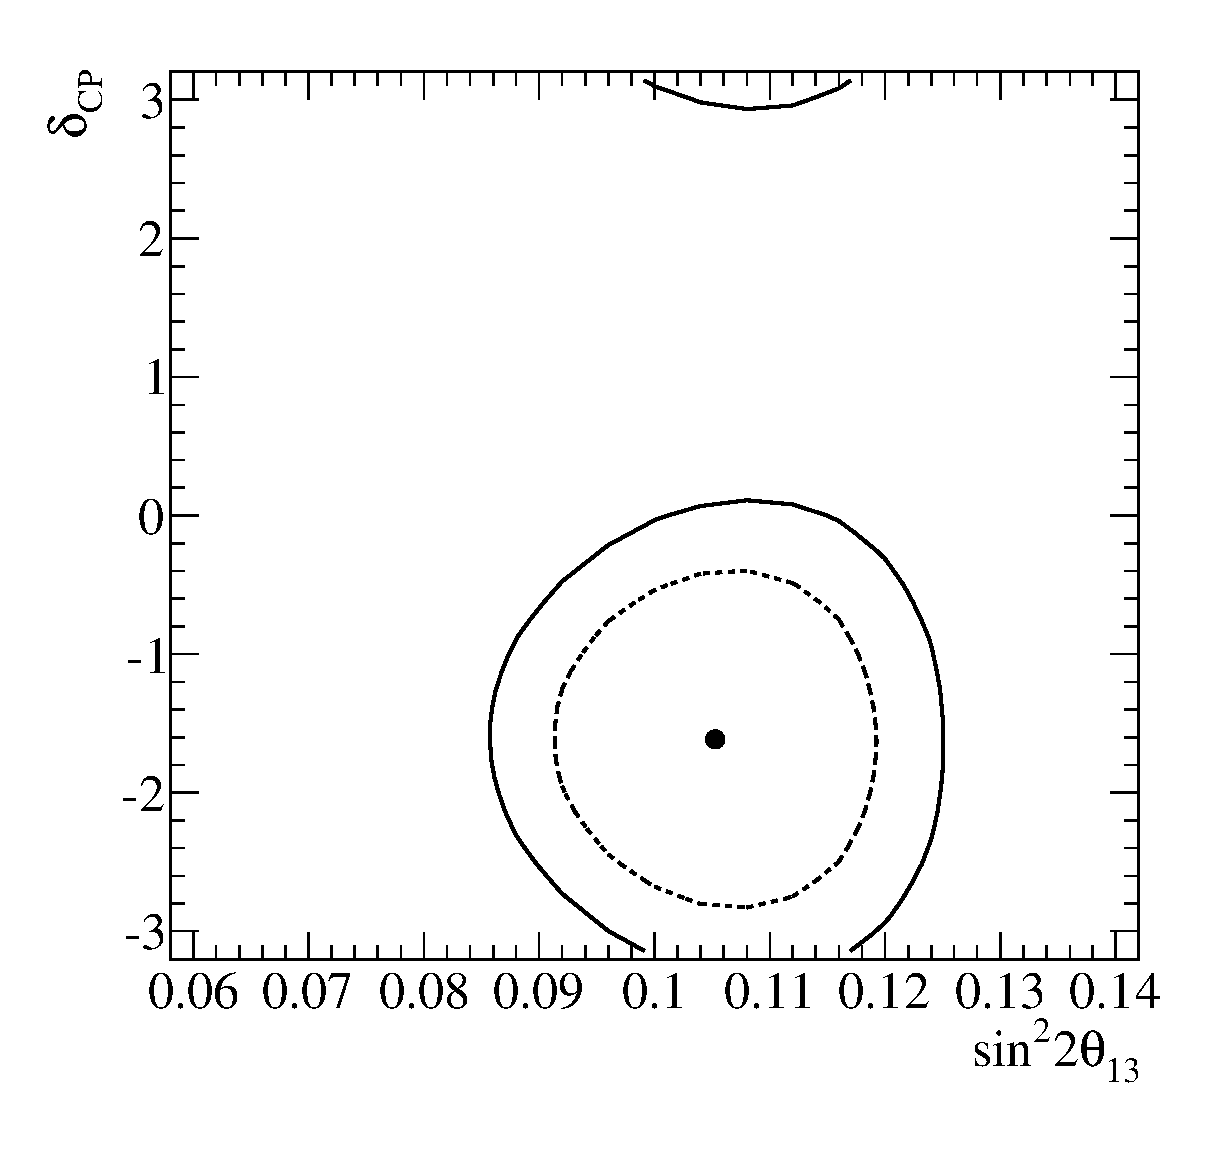
\includegraphics[width=7cm]{./images/validation/toy_dataset4_fit_joint_nh_reactor_2D.eps}
\caption {
 Confidence regions in the ($sin^{2}2\theta_{13}$,$\delta_{CP}$)
parameter space for fake dataset \#4 including constraint in $sin^{2}2\theta_{13}$,
assuming normal hierarchy.
}
\label{fig:validation:toys:reactor_toy4}
\end{minipage}
\hspace{0.02\linewidth}
\begin{minipage}[t]{0.48\linewidth}
\center
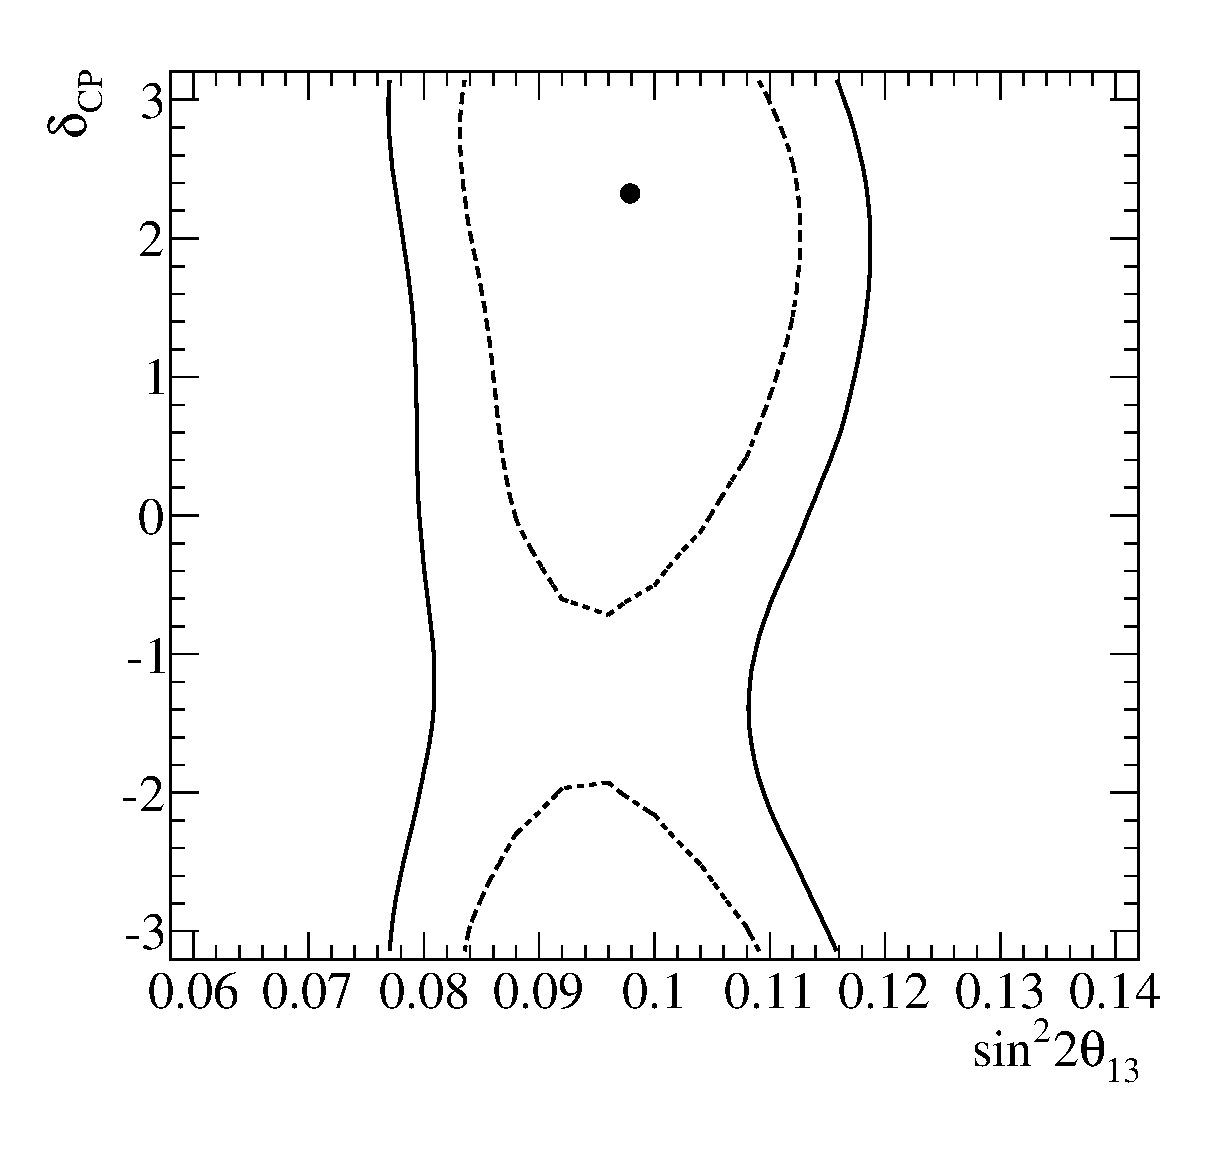
\includegraphics[width=7cm]{./images/validation/toy_dataset5_fit_joint_ih_reactor_2D.eps}
\caption {
 Confidence regions in the ($sin^{2}2\theta_{13}$,$\delta_{CP}$)
parameter space for fake dataset \#5 including constraint in $sin^{2}2\theta_{13}$,
assuming inverted hierarchy.
}
\label{fig:validation:toys:reactor_toy5}
\end{minipage}
\end{figure}




